% !TEX TS-program = LuaLaTeX
\documentclass[11pt,compress,xcolor=x11names,UTF8]{beamer}
\usetheme{Boadilla}
\usecolortheme{seahorse}
\useinnertheme[shadow]{rounded}  
\useoutertheme[subsection=false]{smoothbars}
\usecolortheme{spruce}
\usecolortheme[named=SpringGreen4]{structure}
\usefonttheme{structurebold}
\useinnertheme{circles}
\usecolortheme{rose}
\usepackage{pifont}
\usepackage{academicons}
\usepackage{fontawesome}
\usepackage{iitem}
\usepackage{graphicx}
\usepackage{tabularx}
\setbeamertemplate{itemize item}{\ding{108}}
\setbeamertemplate{itemize subitem}{\ding{109}}
\setbeamertemplate{navigation symbols}{}
\setbeamercovered{transparent}  
\renewcommand\appendixname{附录}
\renewcommand\abstractname{摘要}
\graphicspath{{figure/}} % 图片路径
\usepackage{calligra} % Thank you
\usepackage{ctex} % 加入中文
%\setCJKsansfont{Noto Sans CJK SC}
\setsansfont{Lato} % Lato Roboto Fira Sans
\usepackage{makecell}
\newcommand{\tabincell}[2]{\begin{tabular}{@{}#1@{}}#2\end{tabular}}
\usepackage{url}					
\usepackage{natbib} % 参考文献
%\title[Spatial Generalized Linear Mixed Models]{Spatial Generalized Linear Mixed Models with Application to Prevalence Mapping}
\title{New Method to Calibrate Drawers in Container1}
%\subtitle{奖助金申请答辩}
\author[Rong. Zhao]{Email:zhaor25@mail2.sysu.edu.cn \and  } % \\ 专业:统计学 \\ 方向:数据分析与统计计算
\institute[SYSU]{School of Physics\and } % 理学院\\
\date[\today]{
\includegraphics[width=.5\textwidth]{logo}}

\begin{document}

\maketitle

\begin{frame}{Outline}
\tableofcontents
\end{frame}

\section{Introduction}

%\subsection{研究意义}

\begin{frame}{curent PDE evaluation method}
%\textsf{例} \textbf{例}  \textit{例} 
% \texttt{例}  % 调出仿宋字体了
Currently, we calculate PDE with the formula:
\begin{equation}
PDE={\color{red}PDE_c}\cdot f_{cs}+constant
\label{pde_cs}
\end{equation}
where  $PDE_c$ is the internal PDE result of container and  $f_{cs}$ is the correlation factor between two testing systems.\footnote{We believe the two systems are linear related.}
\vspace{.5cm}

$f_{cs}$ can be obtained by fitting the PDE results of PMTs which were tested in both systems, and it will more precise as the number of tested PMTs increasing.\footnote{smaller statistical error} 
%\begin{table}[]  
%\caption{PMT typical performance}  
%\resizebox{.8\textwidth}{!}{%
%\begin{tabular*}{.98\textwidth}{l|cccc}
%%\toprule  
%\hline  
%\hline  
%Performance & PDE &DCR & TTS& uniformity \\  
%\hline  
%HAMAMATSU &  lower\% & 20 kHz& 3ns& worse \\  
%NNVT  & higher\% & 40kHz & 7ns& better \\  
%\hline  
%\end{tabular*}  
%%}
%\end{table} 
%\begin{figure}
%\centering
%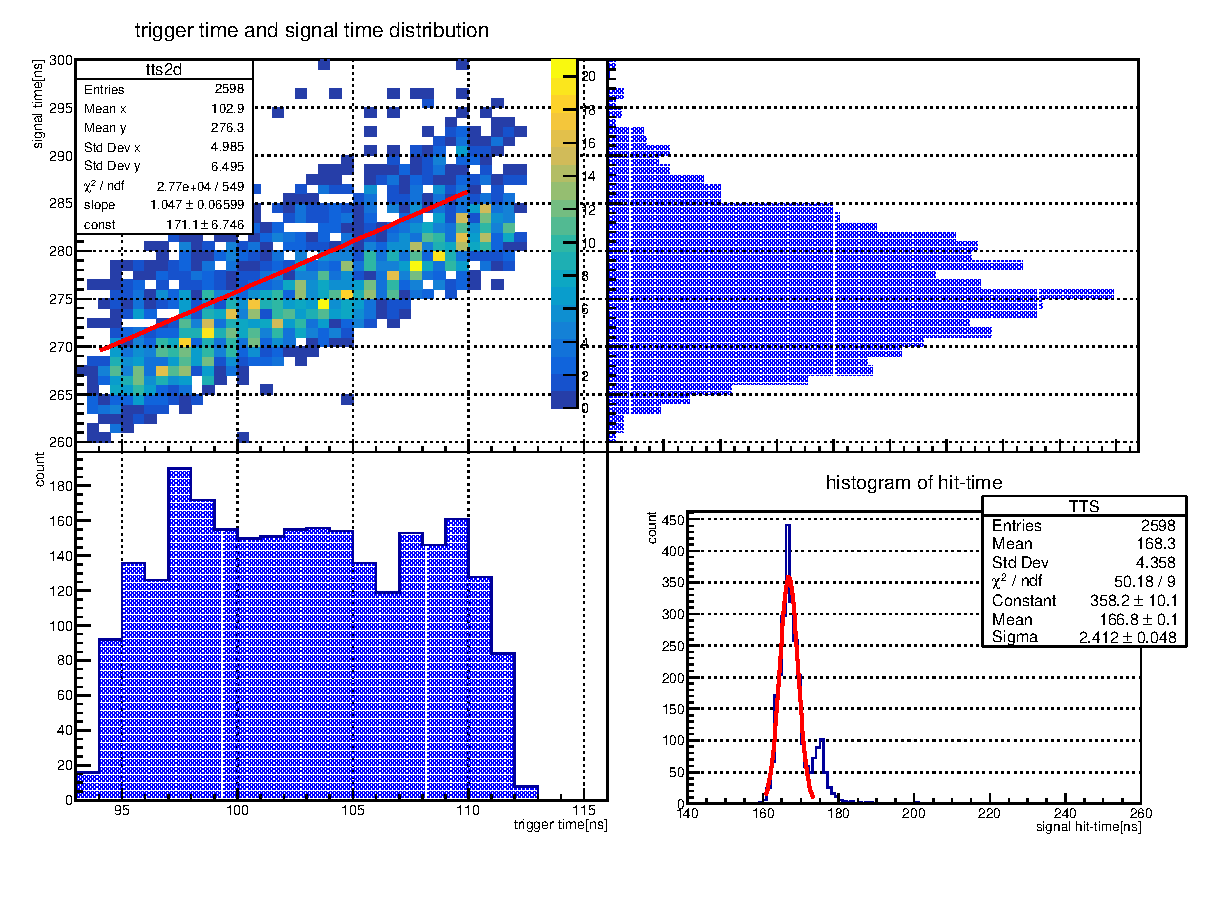
\includegraphics[width=0.78\textwidth]{typical_hittime} % 单图
%\end{figure}
\end{frame}
%%%%%%%%%%%%%%%%%%%%%%%%%%%%%%%%%%%%%%%%%%%
\begin{frame}{current method to calculate $PDE_{c}$}
%\vspace{.5cm}
For each drawer, we get $PDE_c$ using
\begin{equation}
PDE_c=\mu_{test}\cdot {\color{red}drawer_{factor}}
\label{pde_formula}
\end{equation}
where $\mu_{test}$ is the average photon-electron number detected by one PMT,and the $drawer_{factor}$ linearly mapping the $\mu_{test}$ to $PDE_c$。

\vspace{.5cm}
\alert{So, It is very important to precisely calibrate the $drawer_{factor}$. }
\end{frame}
%%%%%%%%%%%%%%%%%%%%%%%%%%%%%%%%%%%%%%%%%%%
\begin{frame}{current method to calibrate $drawer_{factor}$}
Currently we tested 15 HAMAMATSU PMTs with known vendor QE\footnote{check the DocDB file[https://juno.ihep.ac.cn/cgi-bin/Dev\_DocDB/ShowDocument?docid=3646]} in one drawer and fit the QE-$\mu_{test}$results to calculate $drawer_{factor}$.

\vspace{.5cm}

Another choice is {\color{red}to calibrate drawers with all the HAMAMATSU PMTs(with vendor QE) tested in that drawer.}\footnote{}\\
\vspace{.5cm}
The advantage is:systemitic error will decrease as we test more PMTs.\\
The potential risk: we use different PMTs to calibrate different drawers, which may introduces extra uncertainty.

\end{frame}
%%%%%%%%%%%%%%%%%%%%%%%%%%%%%%%%%%%%%%%%%%%
%\begin{frame}{calibration of each drawer}
%Generally, we put several PMTs with known PDE value\footnote{or QE value}  into one drawer and linearly fit the PDE-$\mu_{test}$ data to get \alert{drawer$_{factor}$}. 
%\vspace{.5cm}
%\hrule{\textwidth}
%\vspace{.5cm}
%
%While an alternative way to access the drawer$_{factor}$ is fitting PDE-$\mu_{test}$ data {\color{red}from all the PMTs tested in one drawer rather than the mannual selected ones.} Then once we finish one PMT test in a drawer we will get one more statistical sample in the PDE-$\mu_{test}$ fitting, and we could expect that the fitted drawer$_{factor}$ will get more stable as we testing more PMTs.
%
%\vspace{.5cm}
%The advantage of this "self-calibration" method is that we could {\color{red}decrease the statistical error as much as possible}; and the remained fluctuation of drawer$_{factor}$ can be the system error. 
%\end{frame}
\section{new method to calibrate drawers}
%%%%%%%%%%%%%%%%%%%%%%%%%%%%%%%%%%%%%%%%%%%
\begin{frame}{how to calibrate}
The HAMAMATSU company has provide us with QE\footnote{suppose all the PMTs have same  collection efficiency} value of part of PMTs, which can be downloaded from the PMTtesting data-base.\footnote{wangjun [http://pmtdb.juno.ihep.ac.cn/index.html]} 

\vspace{.5cm}
\hrule{\textwidth}
\vspace{.5cm}
So, once a PMT with vendor QE was tested in the drawer, we can use it to calibrate the drawer. Also, only those PMTs passed the test will be selected.

\vspace{.5cm}
\hrule{\textwidth}
\vspace{.5cm}
After we have the container internal PDE reslts, we need to convert them to final PDE results according to equation \ref{pde_cs}.
\end{frame}
%%%%%%%%%%%%%%%%%%%%%%%%%%%%%%%%%%%%%%%%%%%
\begin{frame}{calibration result of one drawer}
The fitting error will decrease as we test more PMTs, so the drawer factor will be more stable.
\begin{figure}
\centering
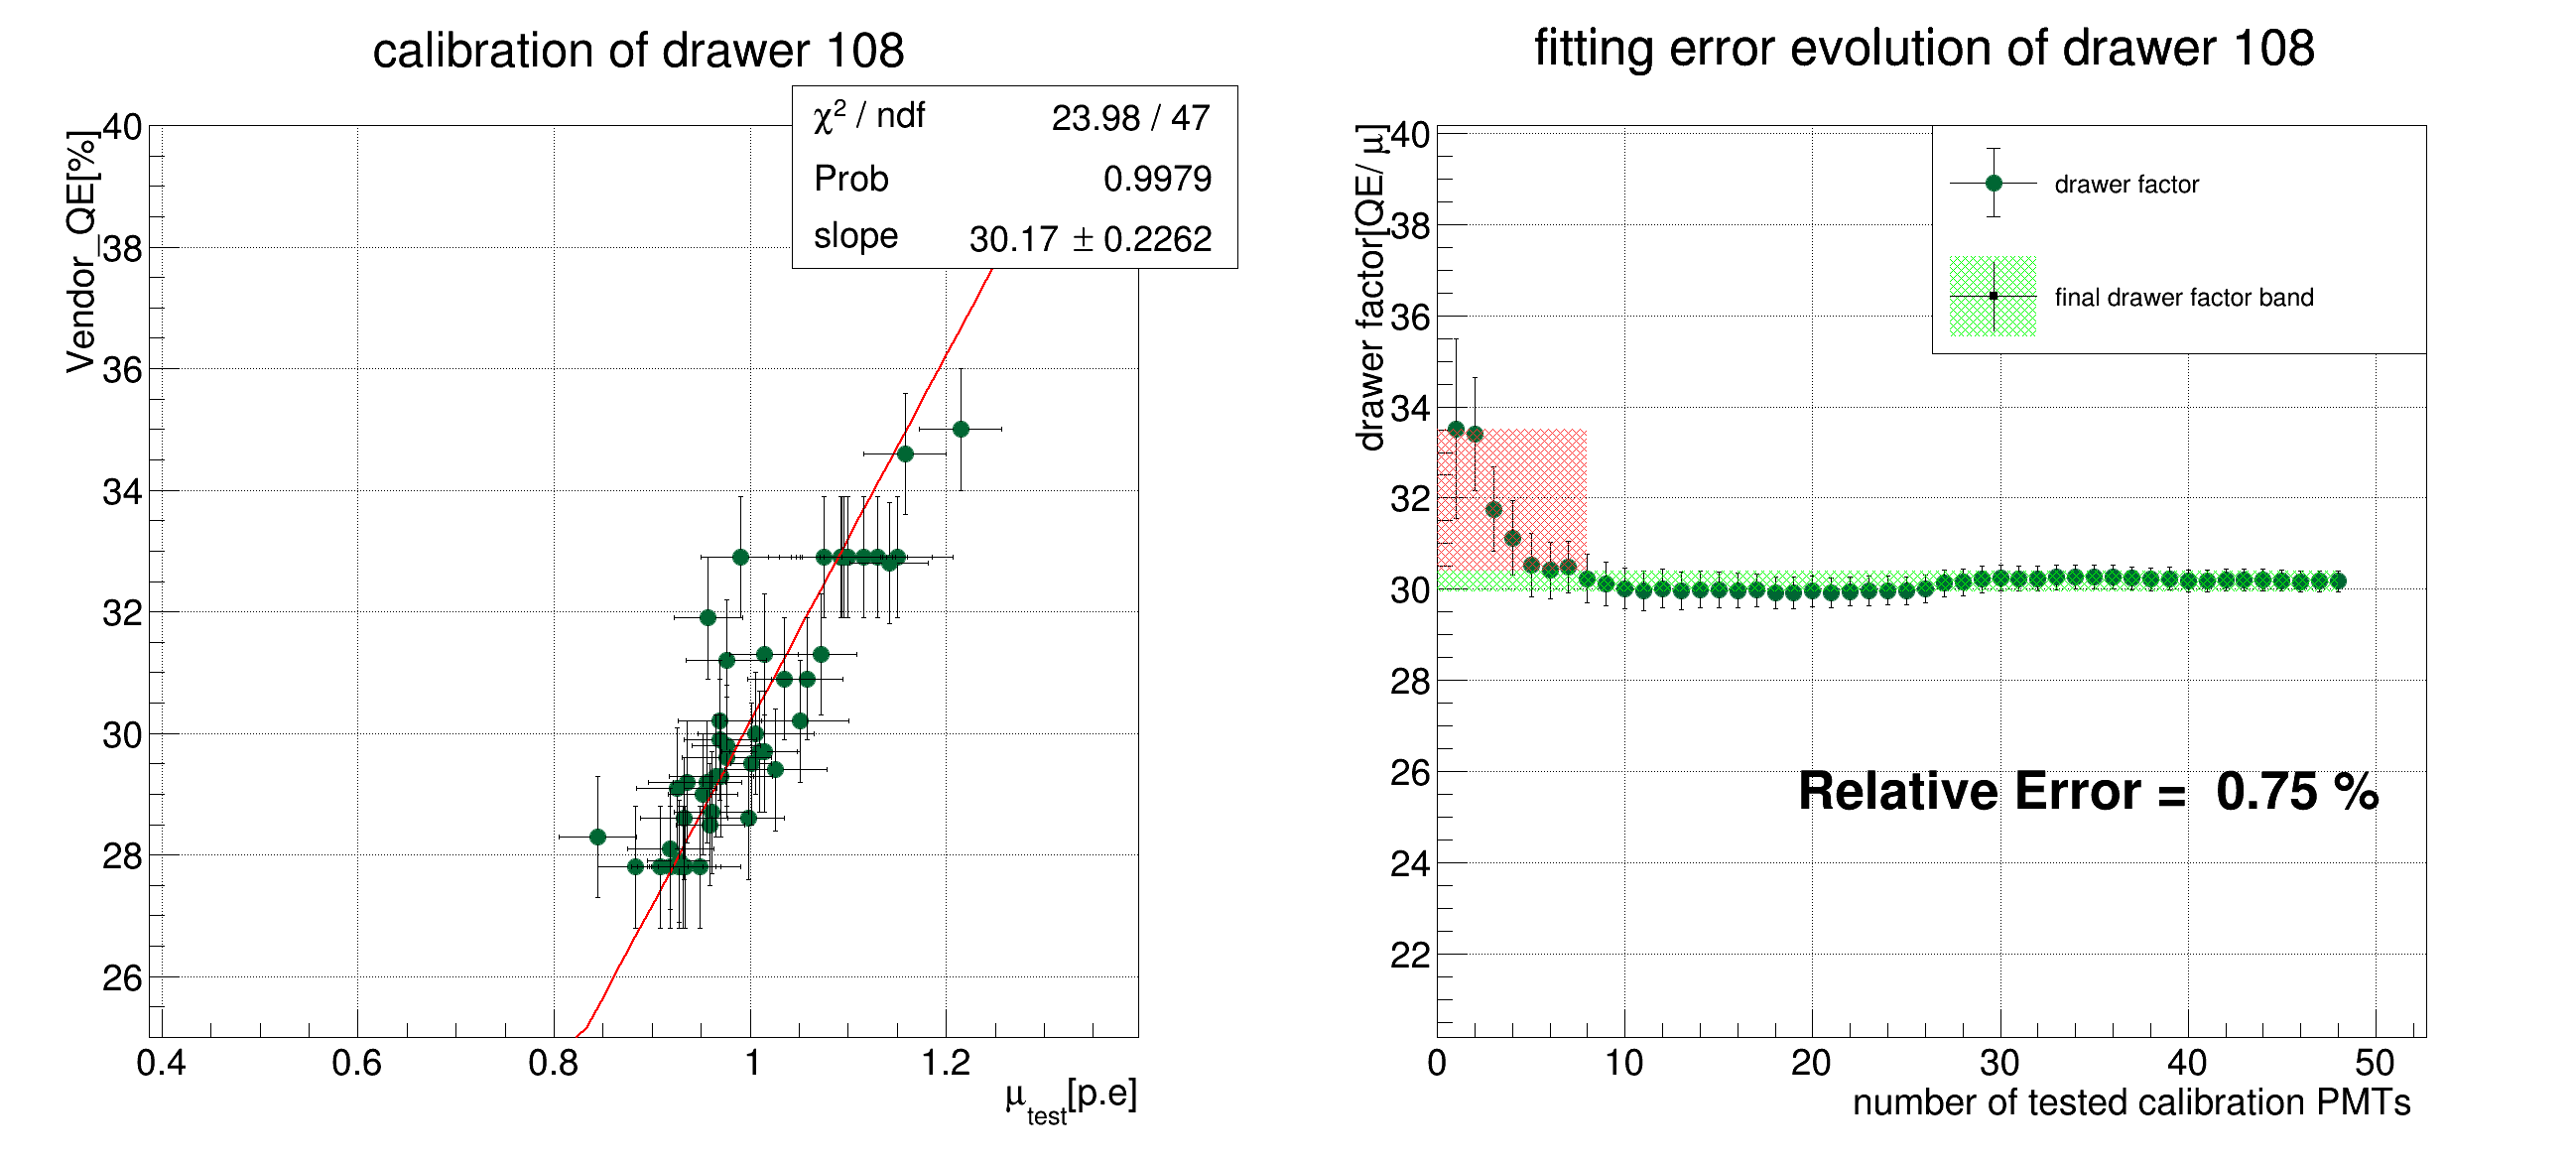
\includegraphics[width=0.98\textwidth]{sta101-7} % 单图
\caption{drawer 108-$drawer_{factor}$}
\end{figure}
\end{frame}
%%%%%%%%%%%%%%%%%%%%%%%%%%%%%%%%%%%%%%%%%%%
%~~!!!!!!!!!!!!!!!!!!put two figures to illustrate!!!!!
\begin{frame}{the calibration results\footnote{comparation with onsite results can be found in back-up section.}}
\begin{columns}
\begin{column}{.5\textwidth}
\begin{figure}
\centering
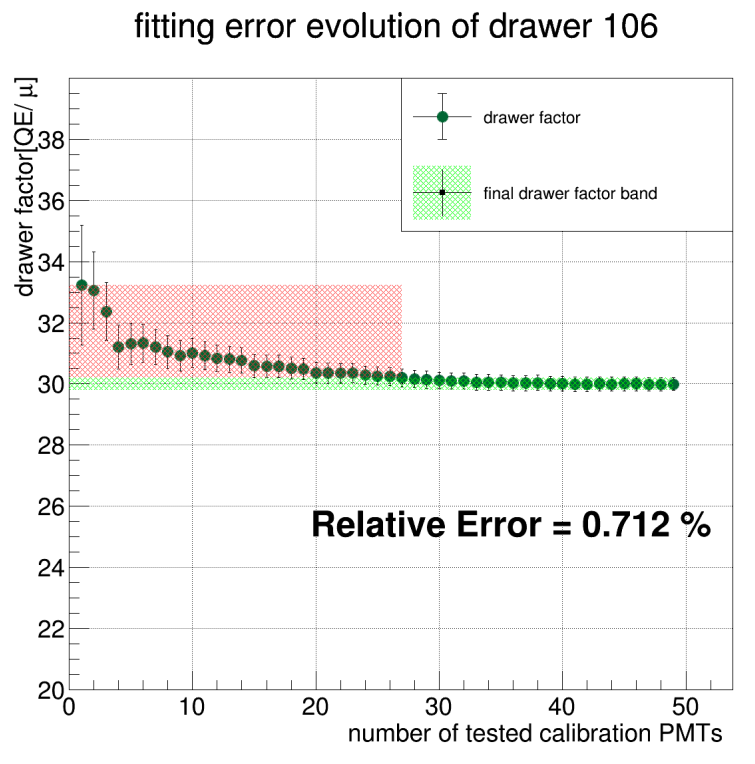
\includegraphics[width=\textwidth]{lt106} % 单图
\end{figure}
\end{column}
\begin{column}{.45\textwidth}
%在某些通道拟合结果会随着事件缓慢上升或者下降(大约1\%),这说明光源强度出现了系统性的漂移。
The $drawer_{factor}$ of some drawer will increase(or decrease) with time slowly(<1\%), this indicates that light intensity of LED may drifted with time. 

\vspace{.5cm}
\hrule{\textwidth}
\vspace{.5cm}

\alert{the fitting error of $drawer_{factor}$ are smaller than 1\%.}

\vspace{.5cm}
\hrule{\textwidth}
\vspace{.5cm}

This means we can monitor the satblity of drawers using the fitting results.

\end{column}
\end{columns}
\end{frame}
%%%%%%%%%%%%%%%%%%%%%%%%%%%%%%%%%%%%%%%%%%%
%~~!!!!!!!!!!!!!!!!!!put two figures to illustrate!!!!!
%\begin{frame}{抽屉刻度结果分析\footnote{拟合出的抽屉因子与现场所使用的抽屉因子的关联见back-up部分}}
%\begin{columns}
%\begin{column}{.5\textwidth}
%\begin{figure}
%\centering
%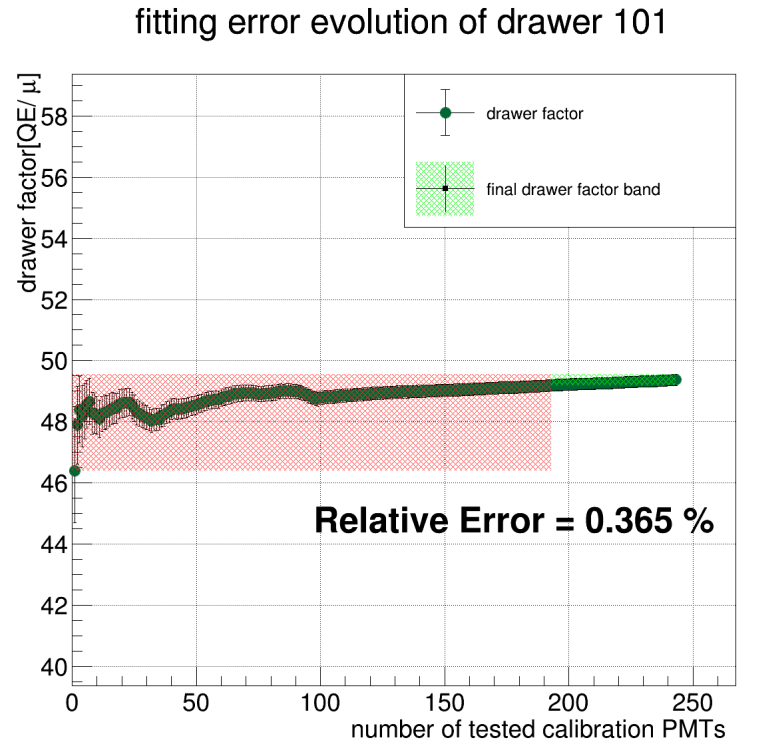
\includegraphics[width=\textwidth]{lt101} % 单图
%\end{figure}
%\end{column}
%\begin{column}{.45\textwidth}
%101抽屉一直放置参考PMT EA0419,抽屉因子$drawer_{factor}$拟合的结果随着时间漂移,这存在两种可能:
%\vspace{.5cm}
%
%\hrule{\textwidth}
%\vspace{.5cm}
%
%另一方面,这样的刻度方法可以用来监控系统的稳定性。因为如果系统稳定工作,拟合系数应该随机涨落。
%
%\end{column}
%\end{columns}
%\end{frame}
%%%%%%%%%%%%%%%%%%%%%%%%%%%%%%%%%%%%%%%%%%%
%~~!!!!!!!!!!!!!!!!!!put two figures to illustrate!!!!!
\begin{frame}{the reference tube EA0419}
\begin{columns}
\begin{column}{.5\textwidth}
\begin{figure}
\centering
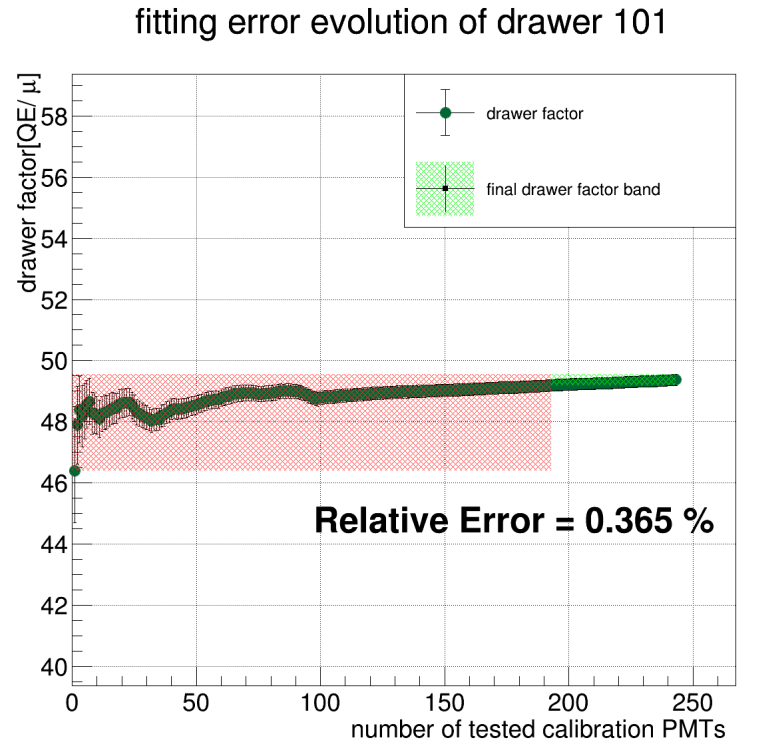
\includegraphics[width=\textwidth]{lt101} % 单图
\end{figure}
\end{column}
\begin{column}{.45\textwidth}
The reference PMT EA0419 was always tested in drawer 101, its fitted $drawer_{factor}$ driftrd slightly with time:
\vspace{.5cm}
\hrule{\textwidth}
\vspace{.5cm}
There are two possible reasons:
\begin{itemize}
\item the LED light intensity decrease with time.
\item PDE of this PMT decrease with time.
\end{itemize}

\end{column}
\end{columns}
\end{frame}
\section{calculation of PDE using this method}
%%%%%%%%%%%%%%%%%%%%%%%%%%%%%%%%%%%%%%%%%%%
%\begin{frame}{calculating the $PDE$}
%After we have the container internal PDE reslts, we need to convert them to final PDE results according to equation \ref{pde_cs}.
%\vspace{.5cm}
%\hrule{\textwidth}
%\vspace{.5cm}
%
%\begin{itemize}
%%\item 因为MCP和HAMAMATSU 两种PMT的性能差异较大,需要对两种PMT分别计算$f_{cs}$。
%\item 使用相同的系数拟合两种PMT,$f_{cs}$=0.897
%\item MCP-PMT 的高量子效率PMT和之前的低量子效率PMT在两个系统的表现不同,需要更多的测量数据进行确认。
%\end{itemize}
%\end{frame}
%%%%%%%%%%%%%%%%%%%%%%%%%%%%%%%%%%%%%%%%%%%
%%%%%%%%%%%%%%%%%%%%%%%%%%%%%%%%%%%%%%%%%%%
\begin{frame}{correlration of results from two testing systems}
By linearly fitting the $PDE_c$ and $PDE_s$ for all the MCP-PMTs, the $f_{cs}$ can be obtained.\footnote{selection criteria:$\Delta PDE<5$}
%\begin{columns}
%\begin{column}{\textwidth}
\begin{figure}
\centering
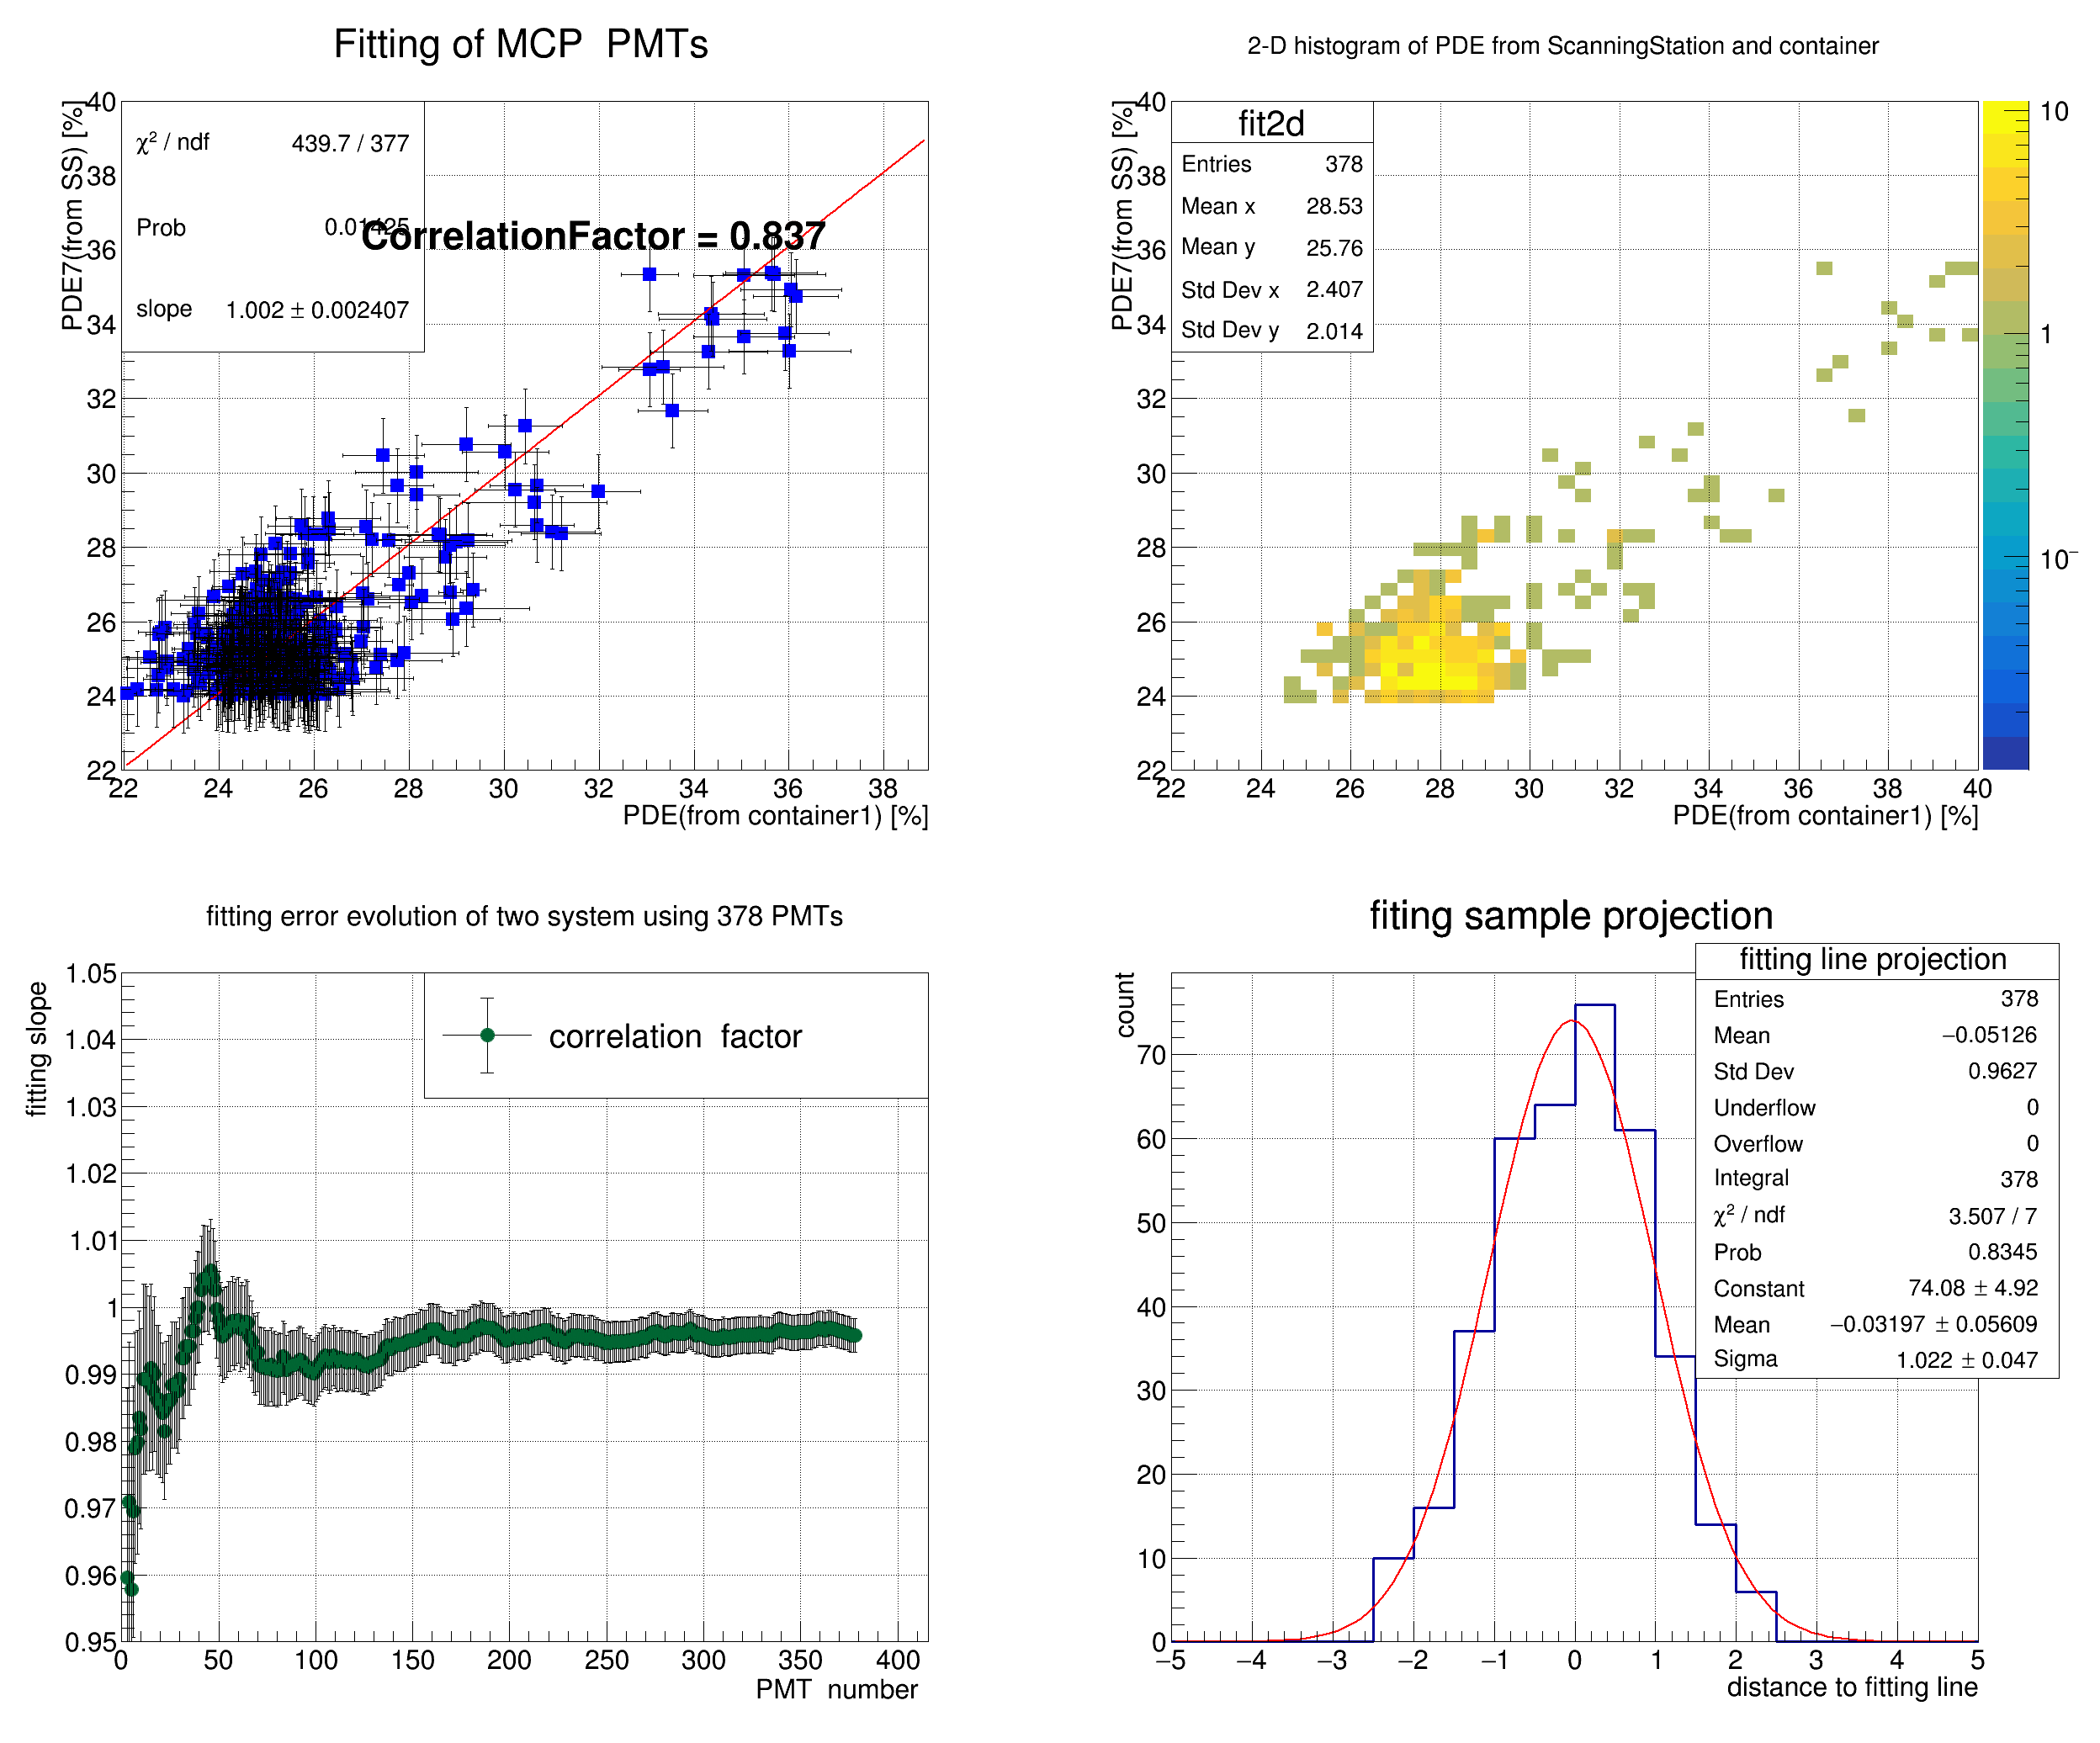
\includegraphics[width=0.58\textwidth]{fit_mcp_noint}
\end{figure}
%\end{column}
%\begin{column}{.001\textwidth}

%\end{column}
%\end{columns}
\end{frame}

%%%%%%%%%%%%%%%%%%%%%%%%%%%%%%%%%%%%%%%%%%%%%%%%%%%%%%%%%%%%%%%%%%%%
\begin{frame}{correlration of results from two testing systems}
%\begin{frame}{两套装置测量结果的转换}
%利用$PDE_c$和$PDE_s$对所有HAMAMATSU-PMT拟合$f_{cs}$的结果\footnote{挑选条件:集装箱测试合格而且$\Delta PDE<5$}:
By linearly fitting the $PDE_c$ and $PDE_s$ for all the HAMAMATSU-PMTs, the $f_{cs}$ can be obtained.\footnote{selection criteria:$\Delta PDE<5$}
\begin{figure}
\centering
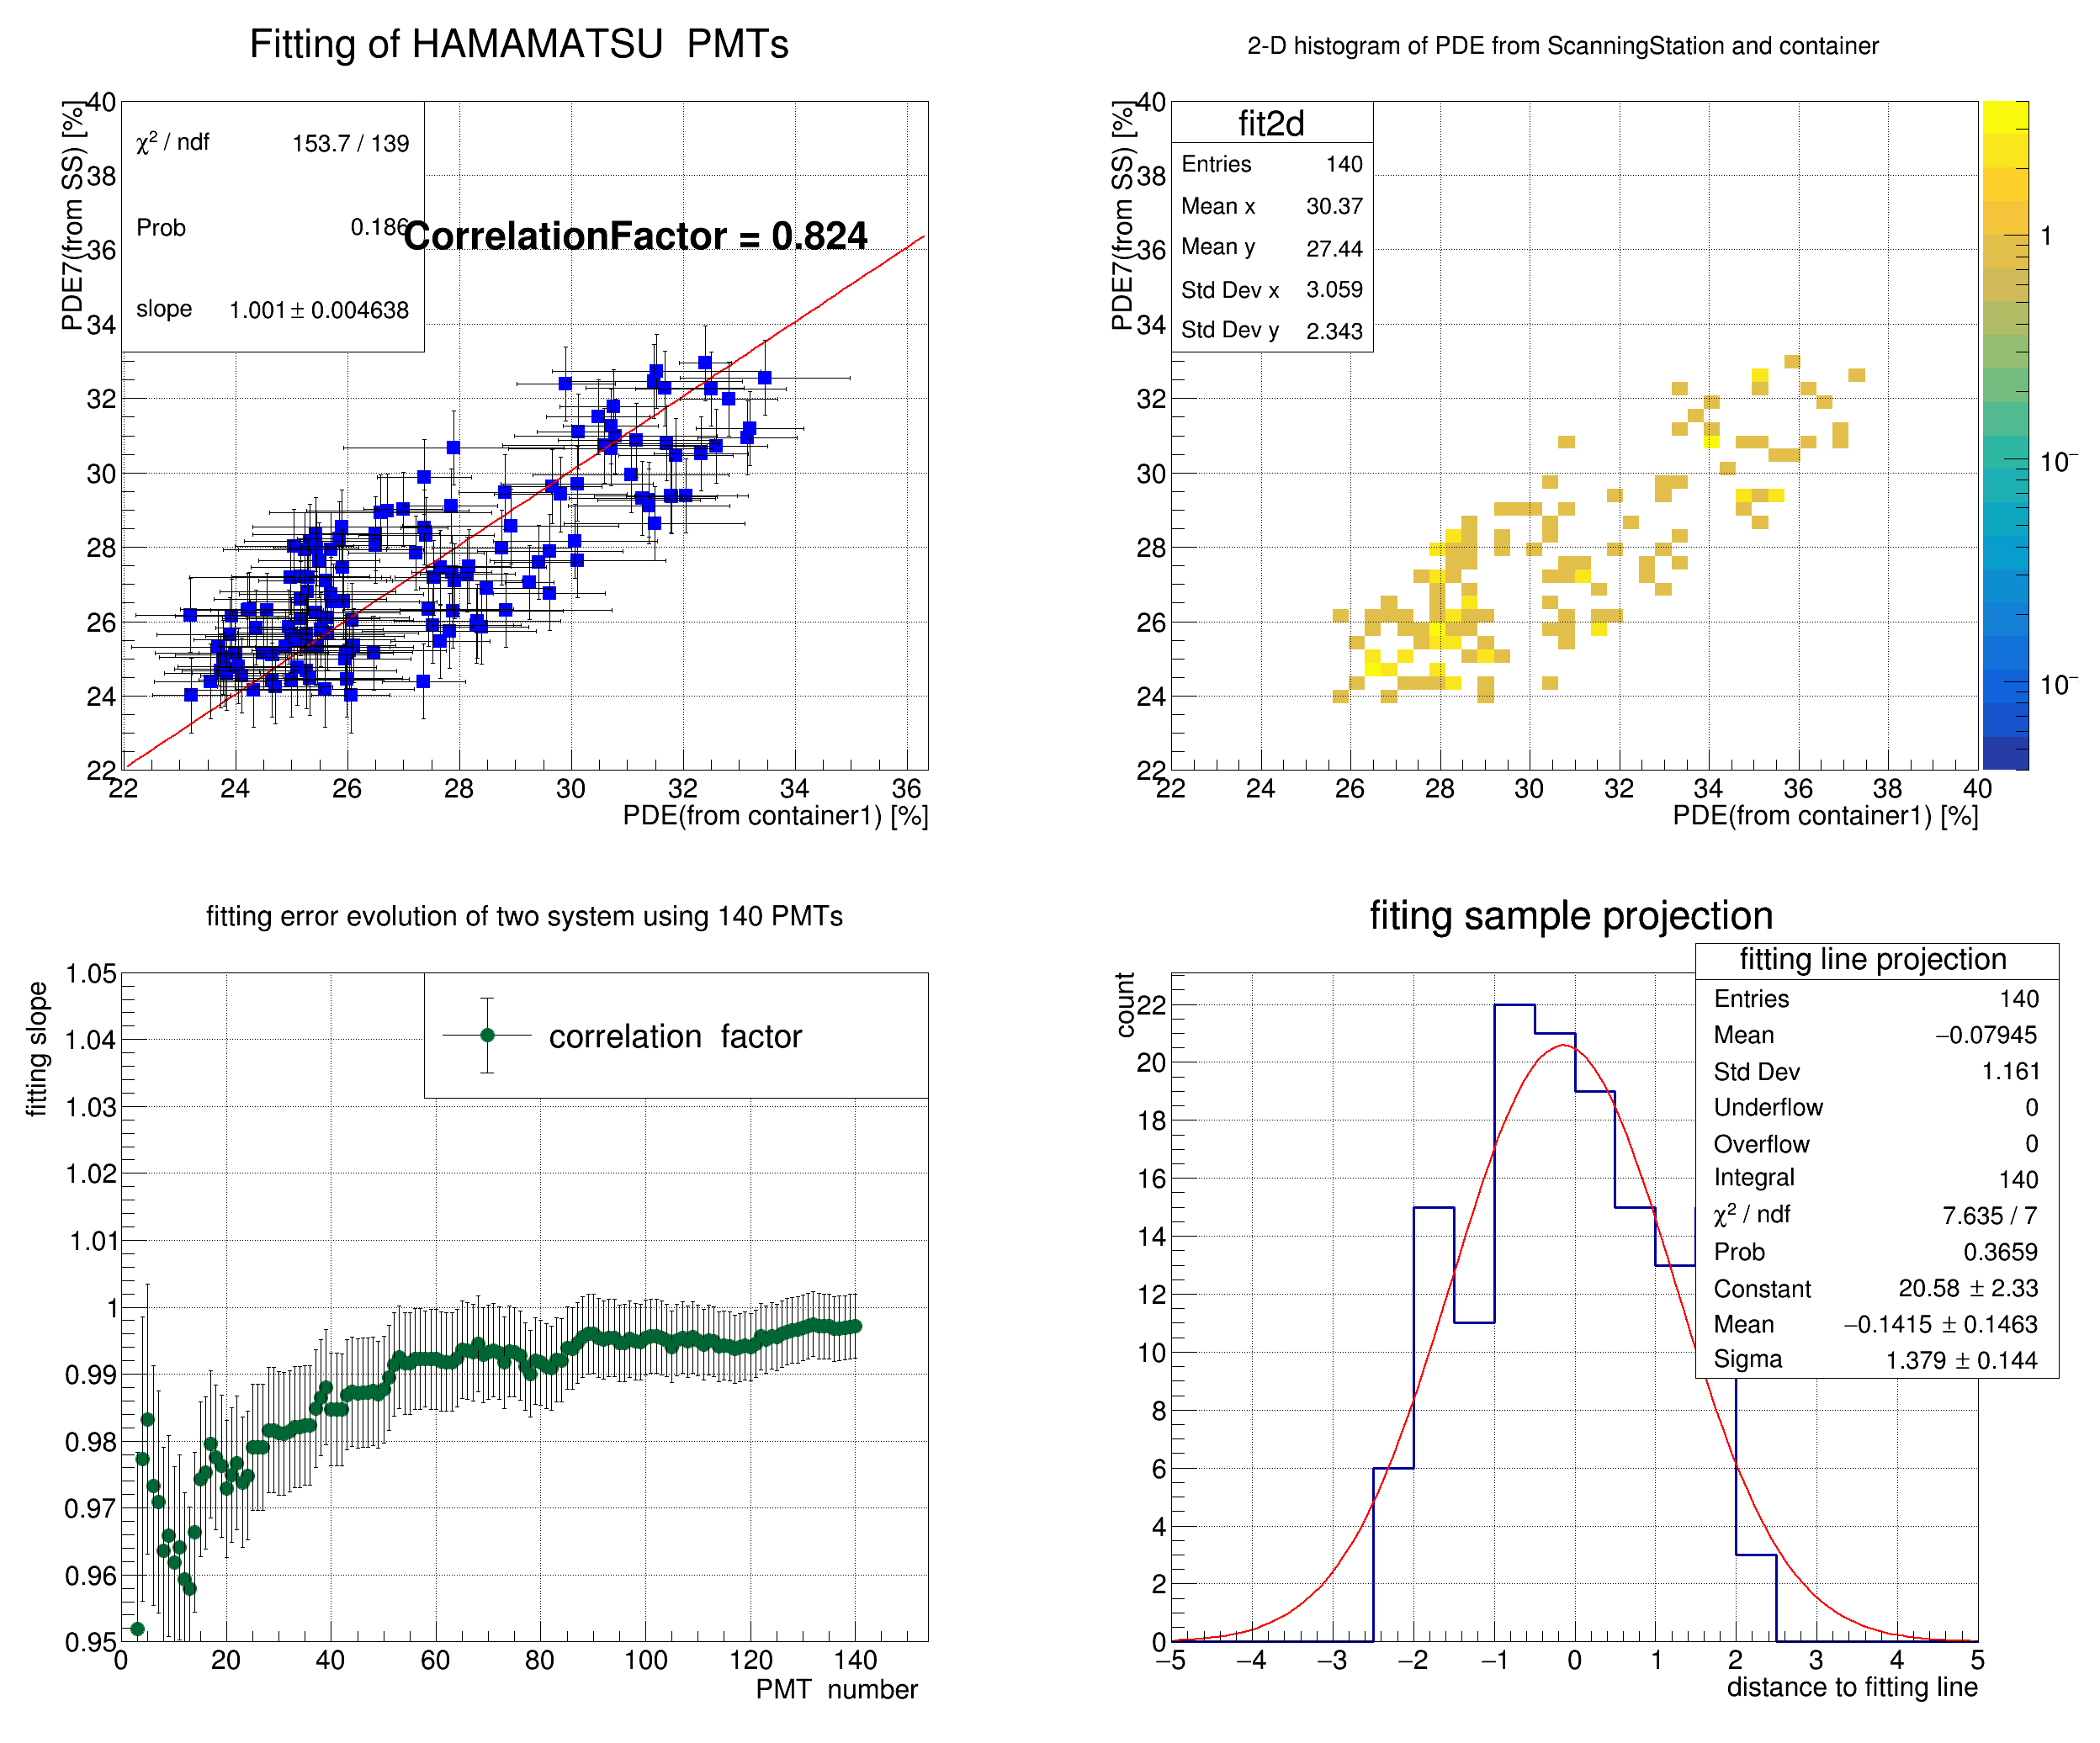
\includegraphics[width=0.58\textwidth]{fit_hmp_noint}
\end{figure}
\end{frame}
%%%%%%%%%%%%%%%%%%%%%%%%%%%%%%%%%%%%%%%%%%%%%%%%%%%%%%%%%%%%%%%%%%%%
%\begin{frame}{两套装置测量结果的转换}
\begin{frame}{correlration of results from two testing systems}
By linearly fitting the $PDE_c$ and $PDE_s$ for all the PMTs, the $f_{cs}$ can be obtained.\footnote{selection criteria:$\Delta PDE<5$}
%利用$PDE_c$和$PDE_s$对所有PMT拟合$f_{cs}$的结果\footnote{挑选条件:集装箱测试合格而且$\Delta PDE<5$}:
\begin{figure}
\centering
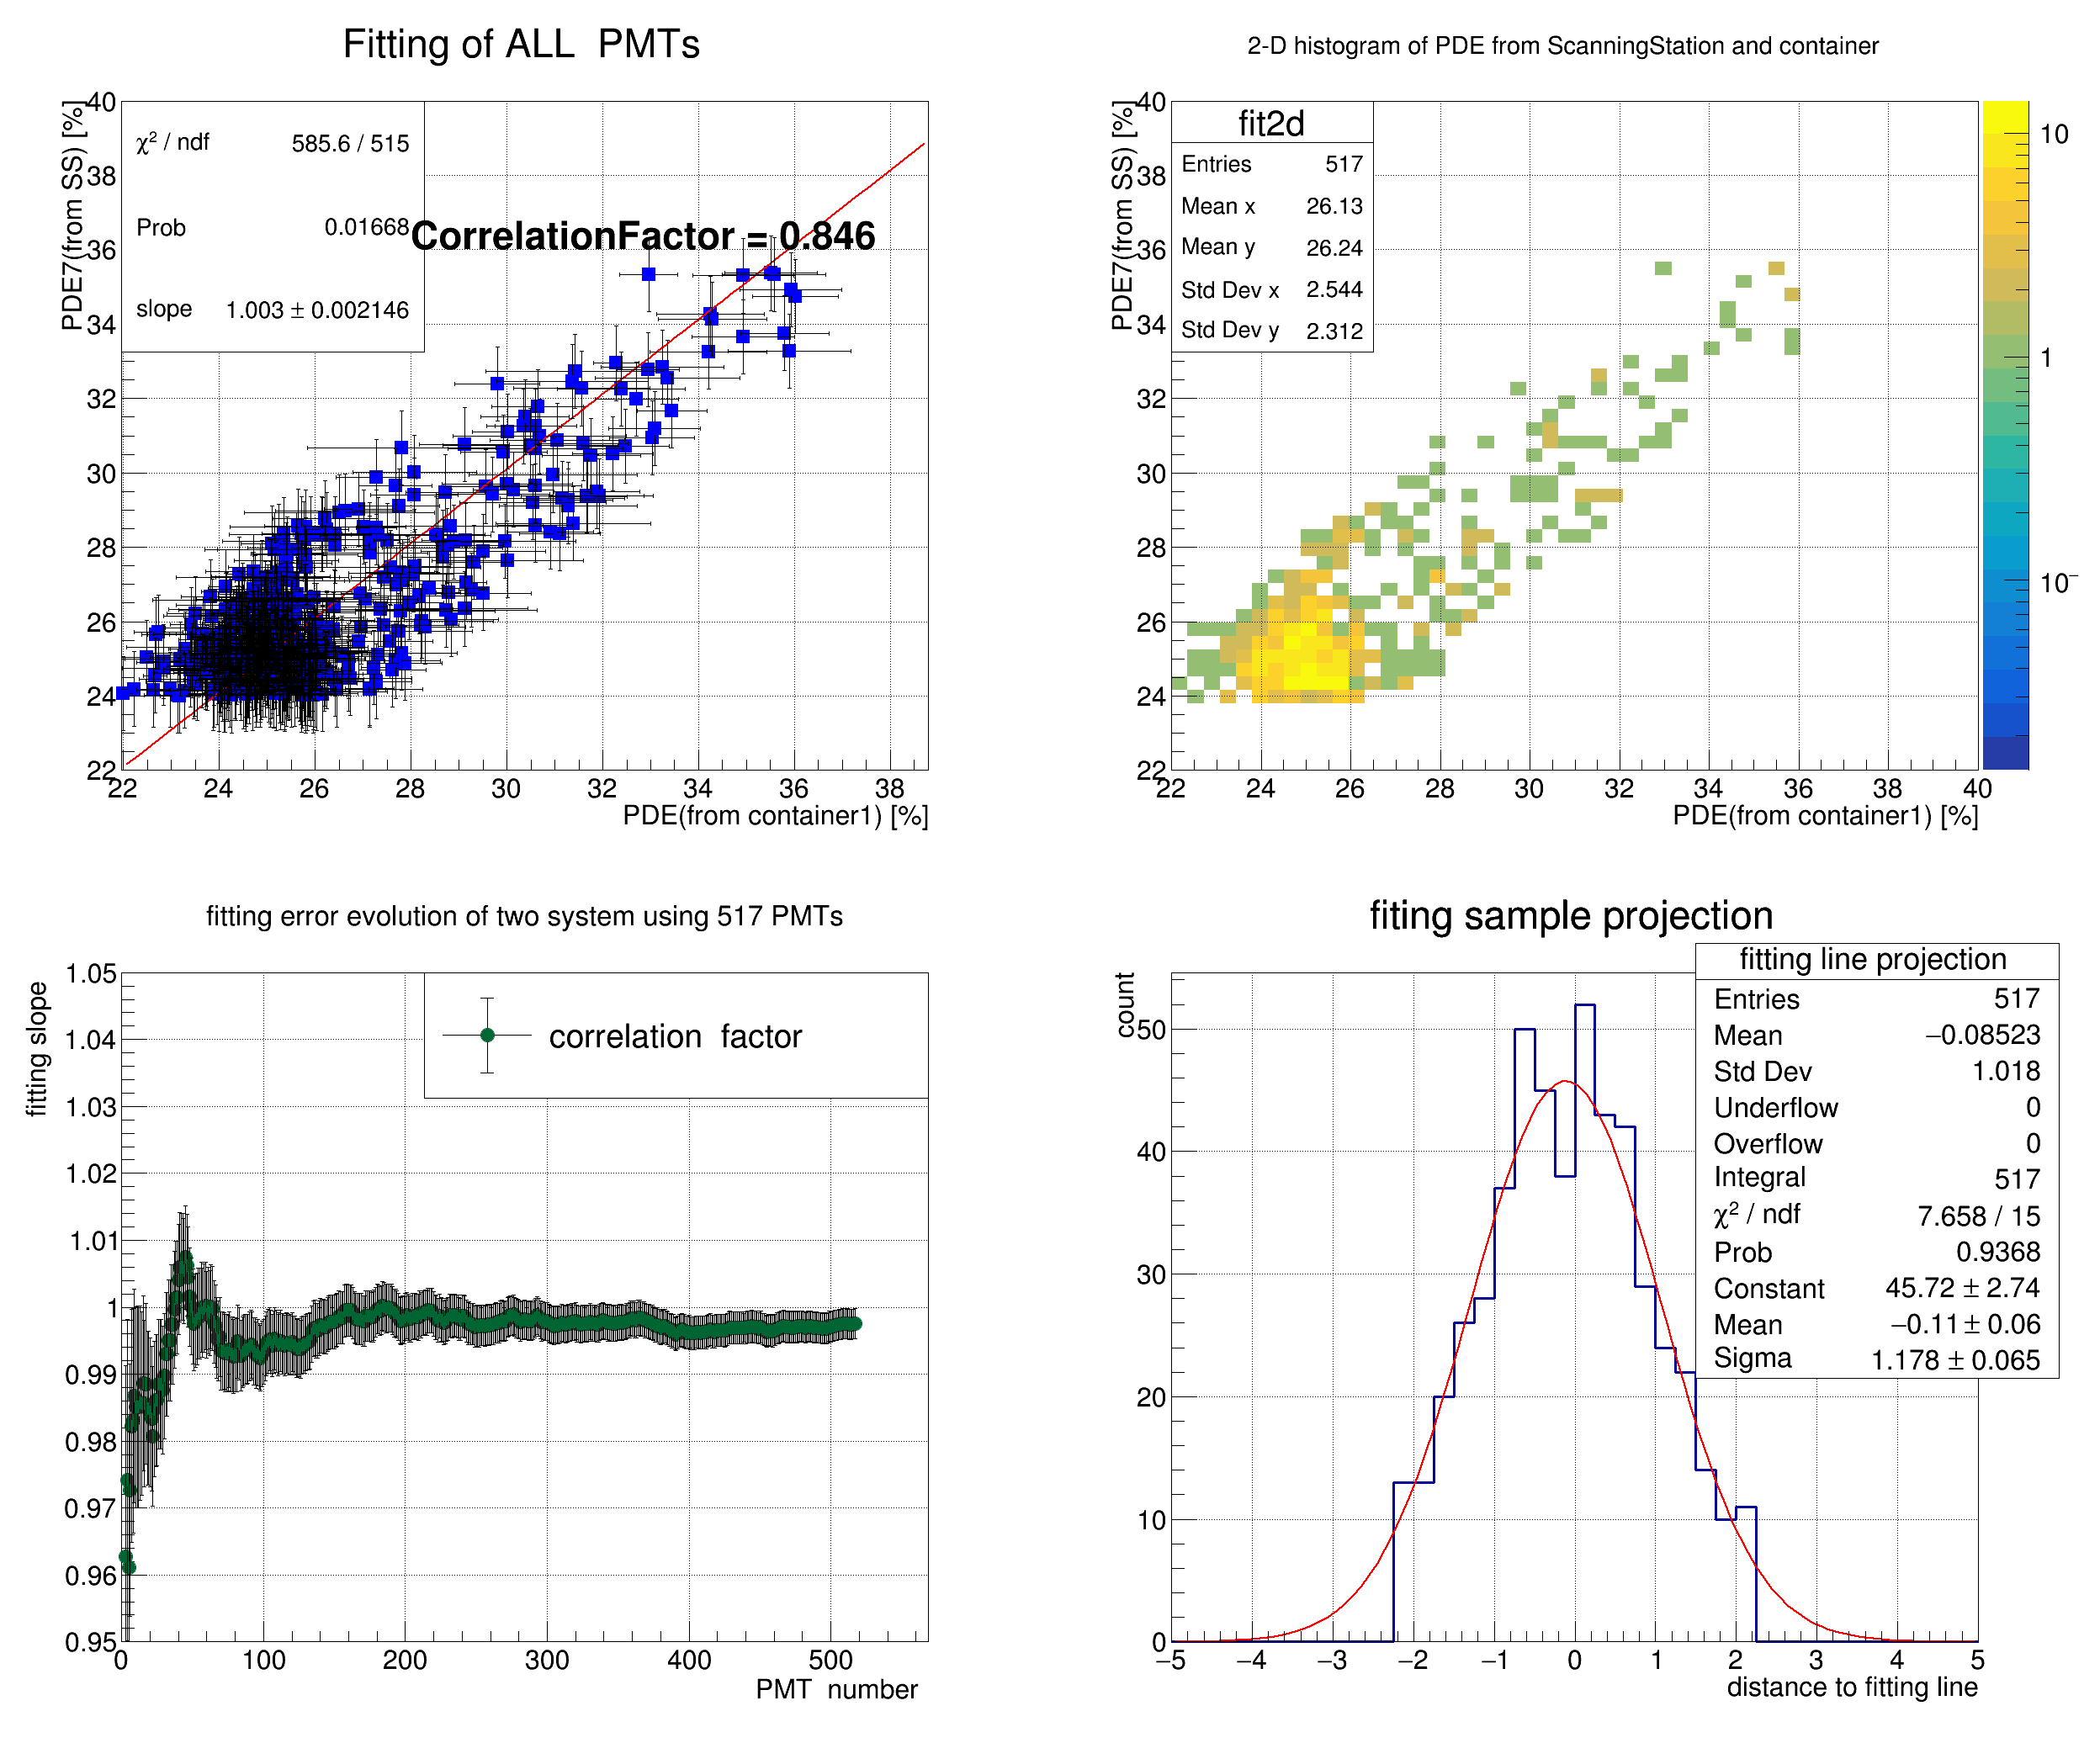
\includegraphics[width=0.58\textwidth]{fit_all_pmts}
\end{figure}
\end{frame}
%%%%%%%%%%%%%%%%%%%%%%%%%%%%%%%%%%%%%%%%%%%%%%%%%%%%%%%%%%%%%%%%%%%%
\begin{frame}{PDE of PMTs}
Once we have $\mu_{test}$ and fitted $drawer_{factor}$,$f_{cs}$ we could get the final PDE of container system:
\hrule{\textwidth}
\begin{figure}
\centering
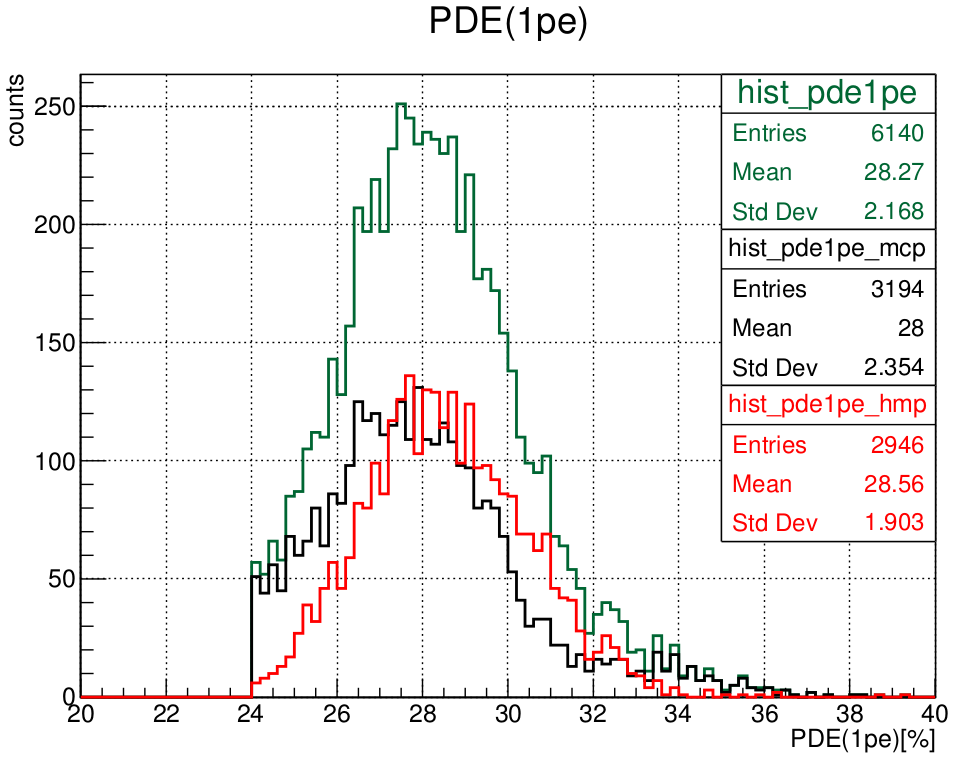
\includegraphics[width=0.45\textwidth]{pde_res}
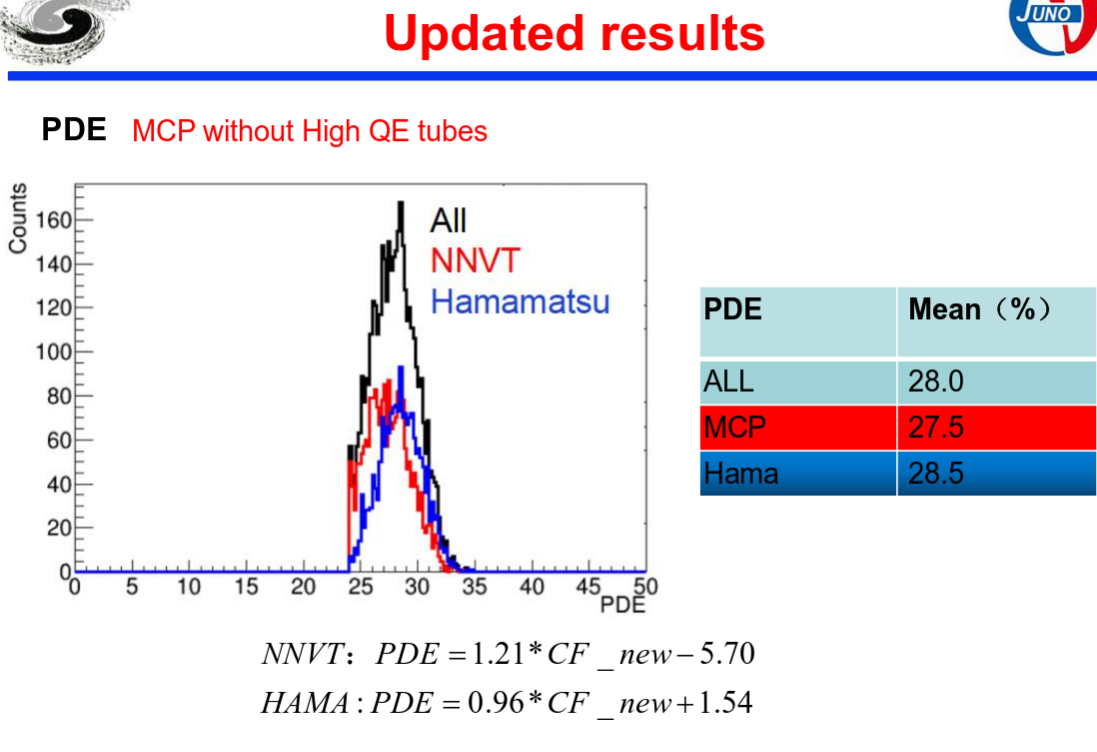
\includegraphics[width=0.45\textwidth]{hqpde}
\caption{left figure shows the PDE results using the new calibration method, right figure shows the onsite PDE results.\footnote{https://juno.ihep.ac.cn/cgi-bin/Dev\_DocDB/ShowDocument?docid=3646}}
\end{figure}
\end{frame}
%%%%%%%%%%%%%%%%%%%%%%%%%%%%%%%%%%%%%%%%%%%%%%%%%%%%%%%%%%%%%%%%%%%%
\begin{frame}{PDE of MCP-PMTs}
The PDE of MCP-PMTs tested in container1 is shown below:\footnote{updated to 2018-10-17}:
%\hrule{\textwidth}
\begin{columns}
\begin{column}{.56\textwidth}
\begin{figure}
\centering
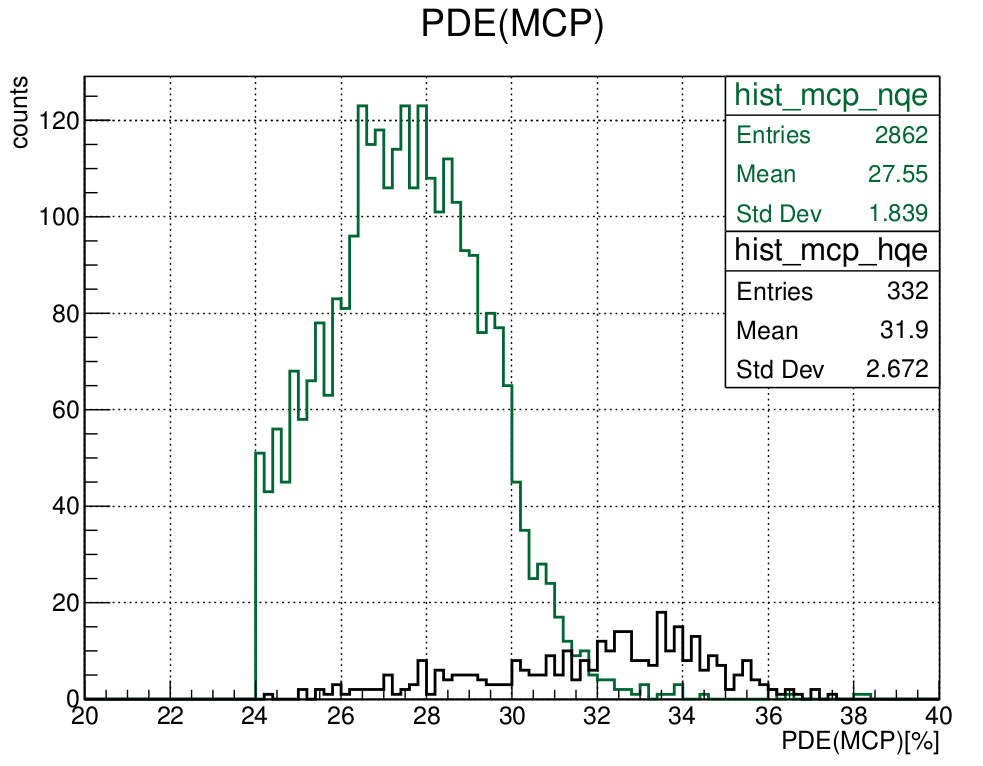
\includegraphics[width=\textwidth]{mcppde}
\end{figure}
\end{column}
\begin{column}{.4\textwidth}
\alert{PDE of High-QE MCP PMTs increase 15.8\%(relative) than one ones.}
\vspace{.5cm}
\hrule{\textwidth}
\vspace{.5cm}
PDE results are consistant with onsite results.\\
MCP:27.5\leftrightarrow \alert{27.55}\\
HAMAMATSU:28.5\leftrightarrow \alert{28.56}
\end{column}
%\end{figure}
\end{columns}
\end{frame}
%%%%%%%%%%%%%%%%%%%%%%%%%%%%%%%%%%%%%%%%%%%%%%%%%%%%%%%%%%%%%%%
%%%%%%%%%%%%%%%%%%%%%%%%%%%%%%%%%%%%%%%%%%%%%%%%%%%%%%%%%%%%%%%
\section{summary}

\begin{frame}{summary and conclusions}
\begin{itemize}
\item fitting the $drawer_{factor}$ using PMTs tested in this drawer, fitting error <1\%.
\item this calibration method can decrease the drawer factor fitting error and could be used to monitor the stability of drawers.
\item the PDE from this calibration is consistant with onsite results(relative error <1\%).
\item High-QE version MCP PMTs have relatively 17.78\% higher PDE than old ones, the average PDE is about 31.9\%\footnote{onsite result is 32.6\%}
\end{itemize}
\end{frame}

\begin{frame}
\centering {\zihao{0} \color{red} \calligra{THANKS}}
\end{frame}

\begin{frame}
\centering {\zihao{0} \color{red} \calligra{BACK-UP}}
\end{frame}

%\begin{frame}[allowframebreaks]
%\frametitle{References}
%\scriptsize
%\bibliographystyle{authordate1}
%\bibliography{R-GLMM-pkgs}
%\end{frame}

\appendix

\section*{附录}

\begin{frame}{check of other parameters}
HAMAMATSU-PMT:

\vspace{.5cm}

\centering
\begin{tabular}{l|c|c}
\hline
\hline
parameters(average)&  {\color{Blue} my results} & {\color{Blue}onsite results} \\\hline
dark count rate(kHz)&17.8&16.6\\
rise time(ns)&7.3& 6.9\\
fall time(ns)&10.36& 10.2\\
peak-valley ratio&3.3& 3.9\\
resolution&0.28& 0.277\\
high voltage(V)&1861& 1858\\
signal FWHM(ns)&9.08& 11.6\\
\hline
\end{tabular}

%\begin{table}[htbp]  
%\caption{PMT typical performance}  
%\resizebox{.8\textwidth}{!}{%
%\begin{tabular*}{.98\textwidth}{l|cccc}
%%\toprule  
%\hline  
%\hline  
%Performance & PDE &DCR & TTS& uniformity \\  
%\hline  
%HAMAMATSU &  lower\% & 20 kHz& 3ns& worse \\  
%NNVT  & higher\% & 40kHz & 7ns& better \\  
%\hline  
%\end{tabular*}  
%%}
%\end{table} 

\end{frame}
\begin{frame}{check of other parameters}
MCP-PMT:

\vspace{.5cm}

\centering
\begin{tabular}{l|c|c}
\hline
\hline
parameters(average)&  {\color{Blue} my results} & {\color{Blue}onsite results} \\\hline
dark count rate(kHz)&41.4&44.3\\
rise time(ns)&3.2& 4.6\\
fall time(ns)&15.9& 16.2\\
peak-valley ratio3.19& 4.4\\
resolution&0.35& 0.32\\
high voltage(V)&1783& 1784\\
signal FWHM(ns)&5.8& 7.7\\
\hline
\end{tabular}
\end{frame}
\begin{frame}{drawer-calibration}
\vspace{-.5cm}
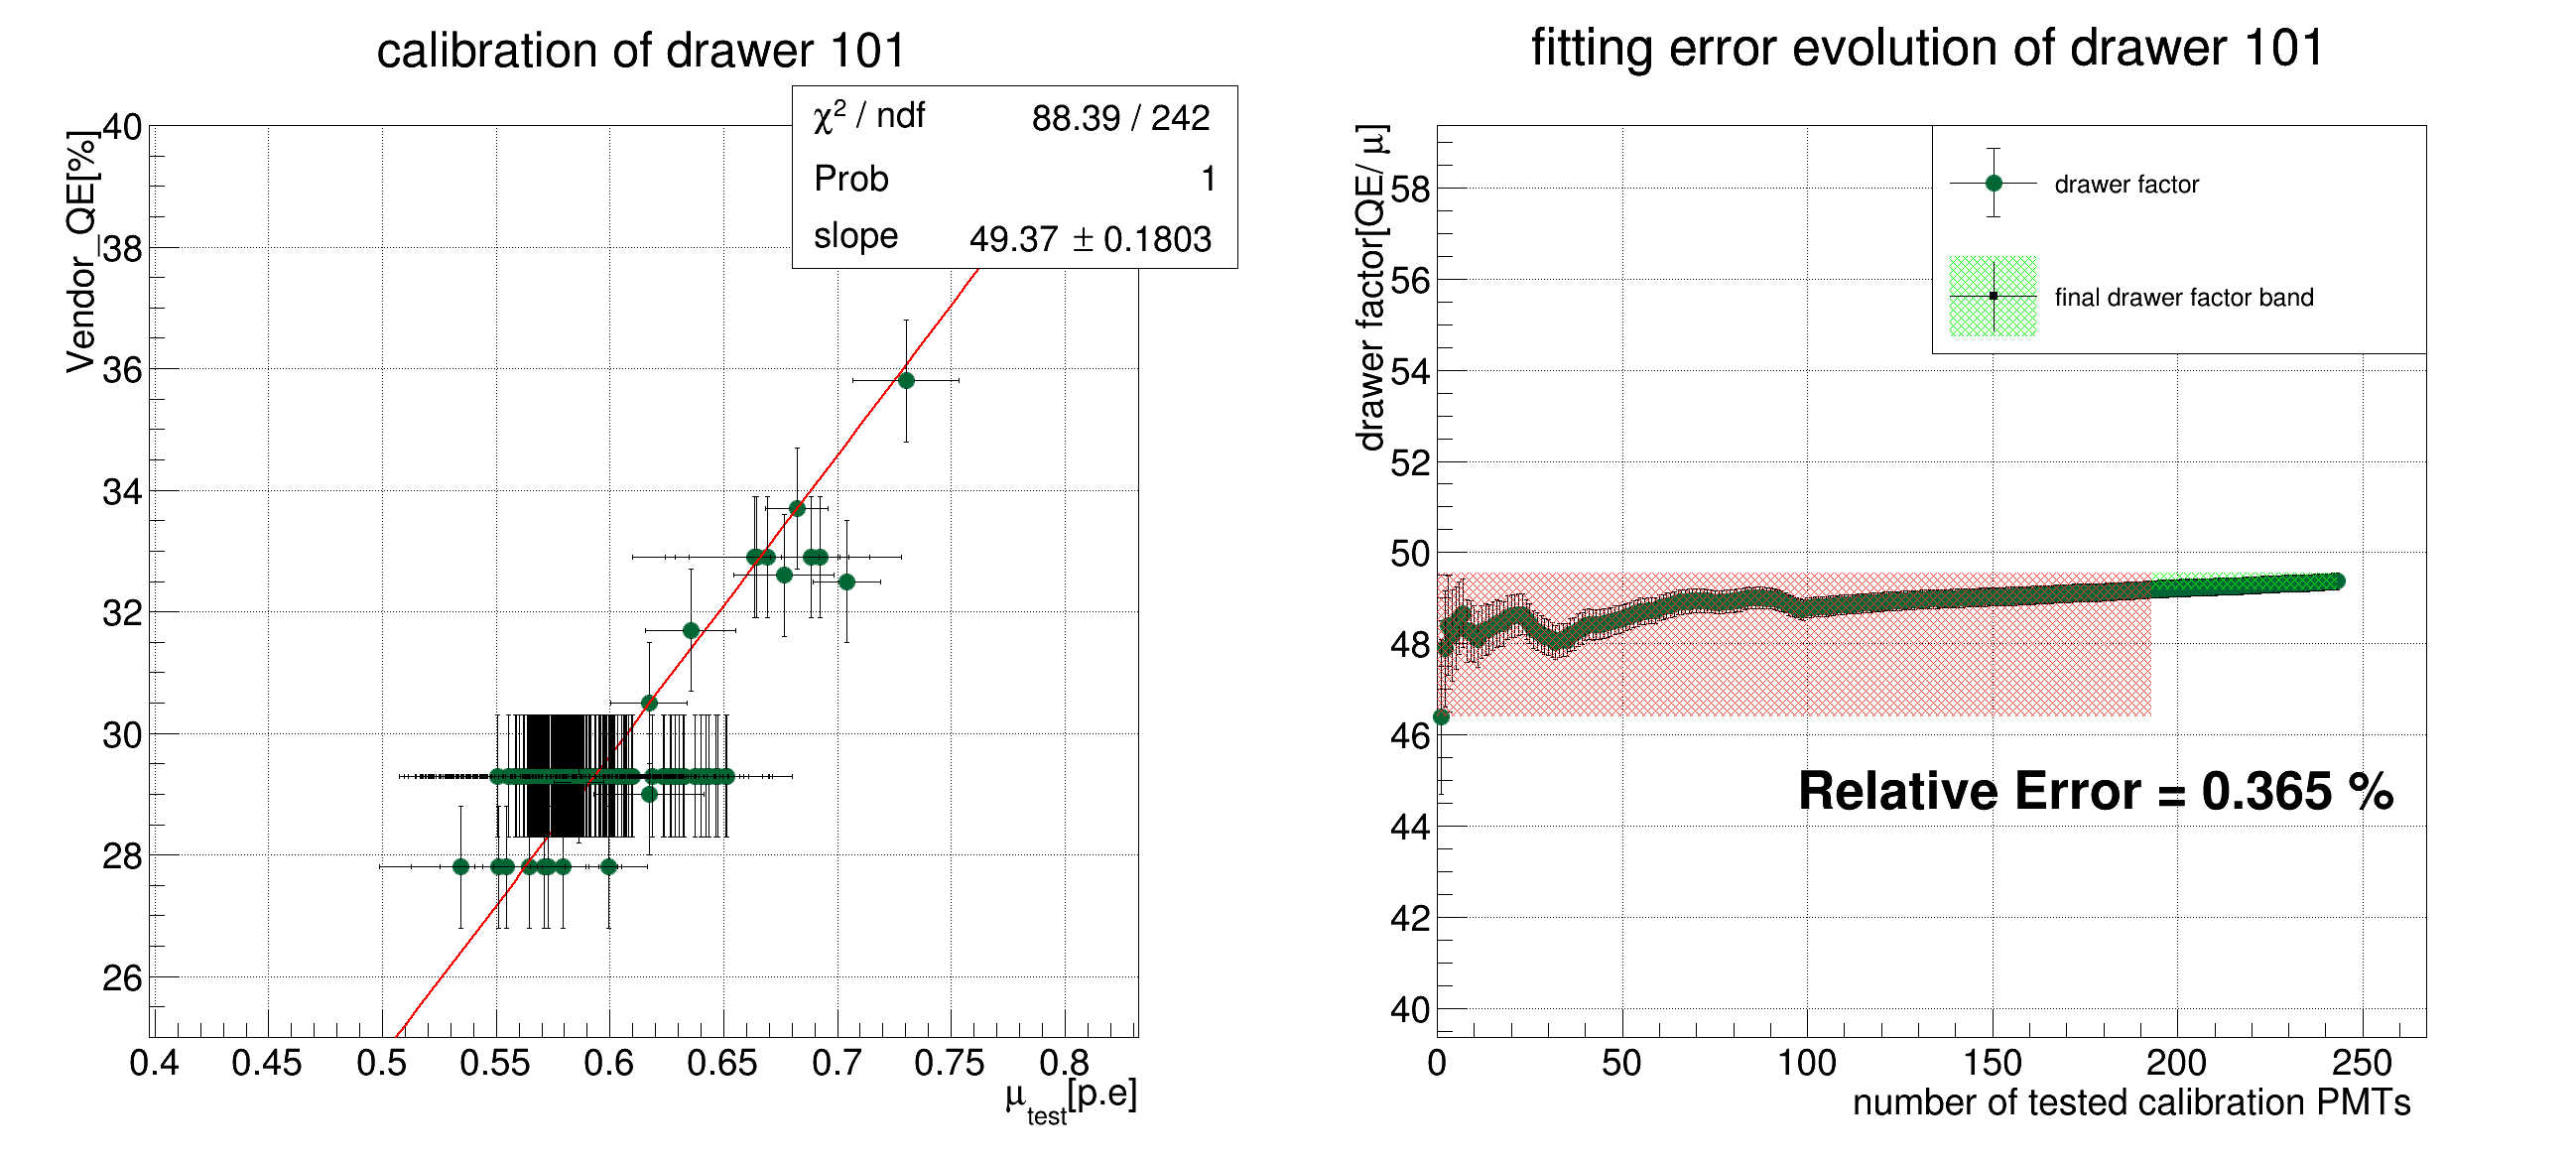
\includegraphics[width=0.45\textwidth]{sta101-0} 
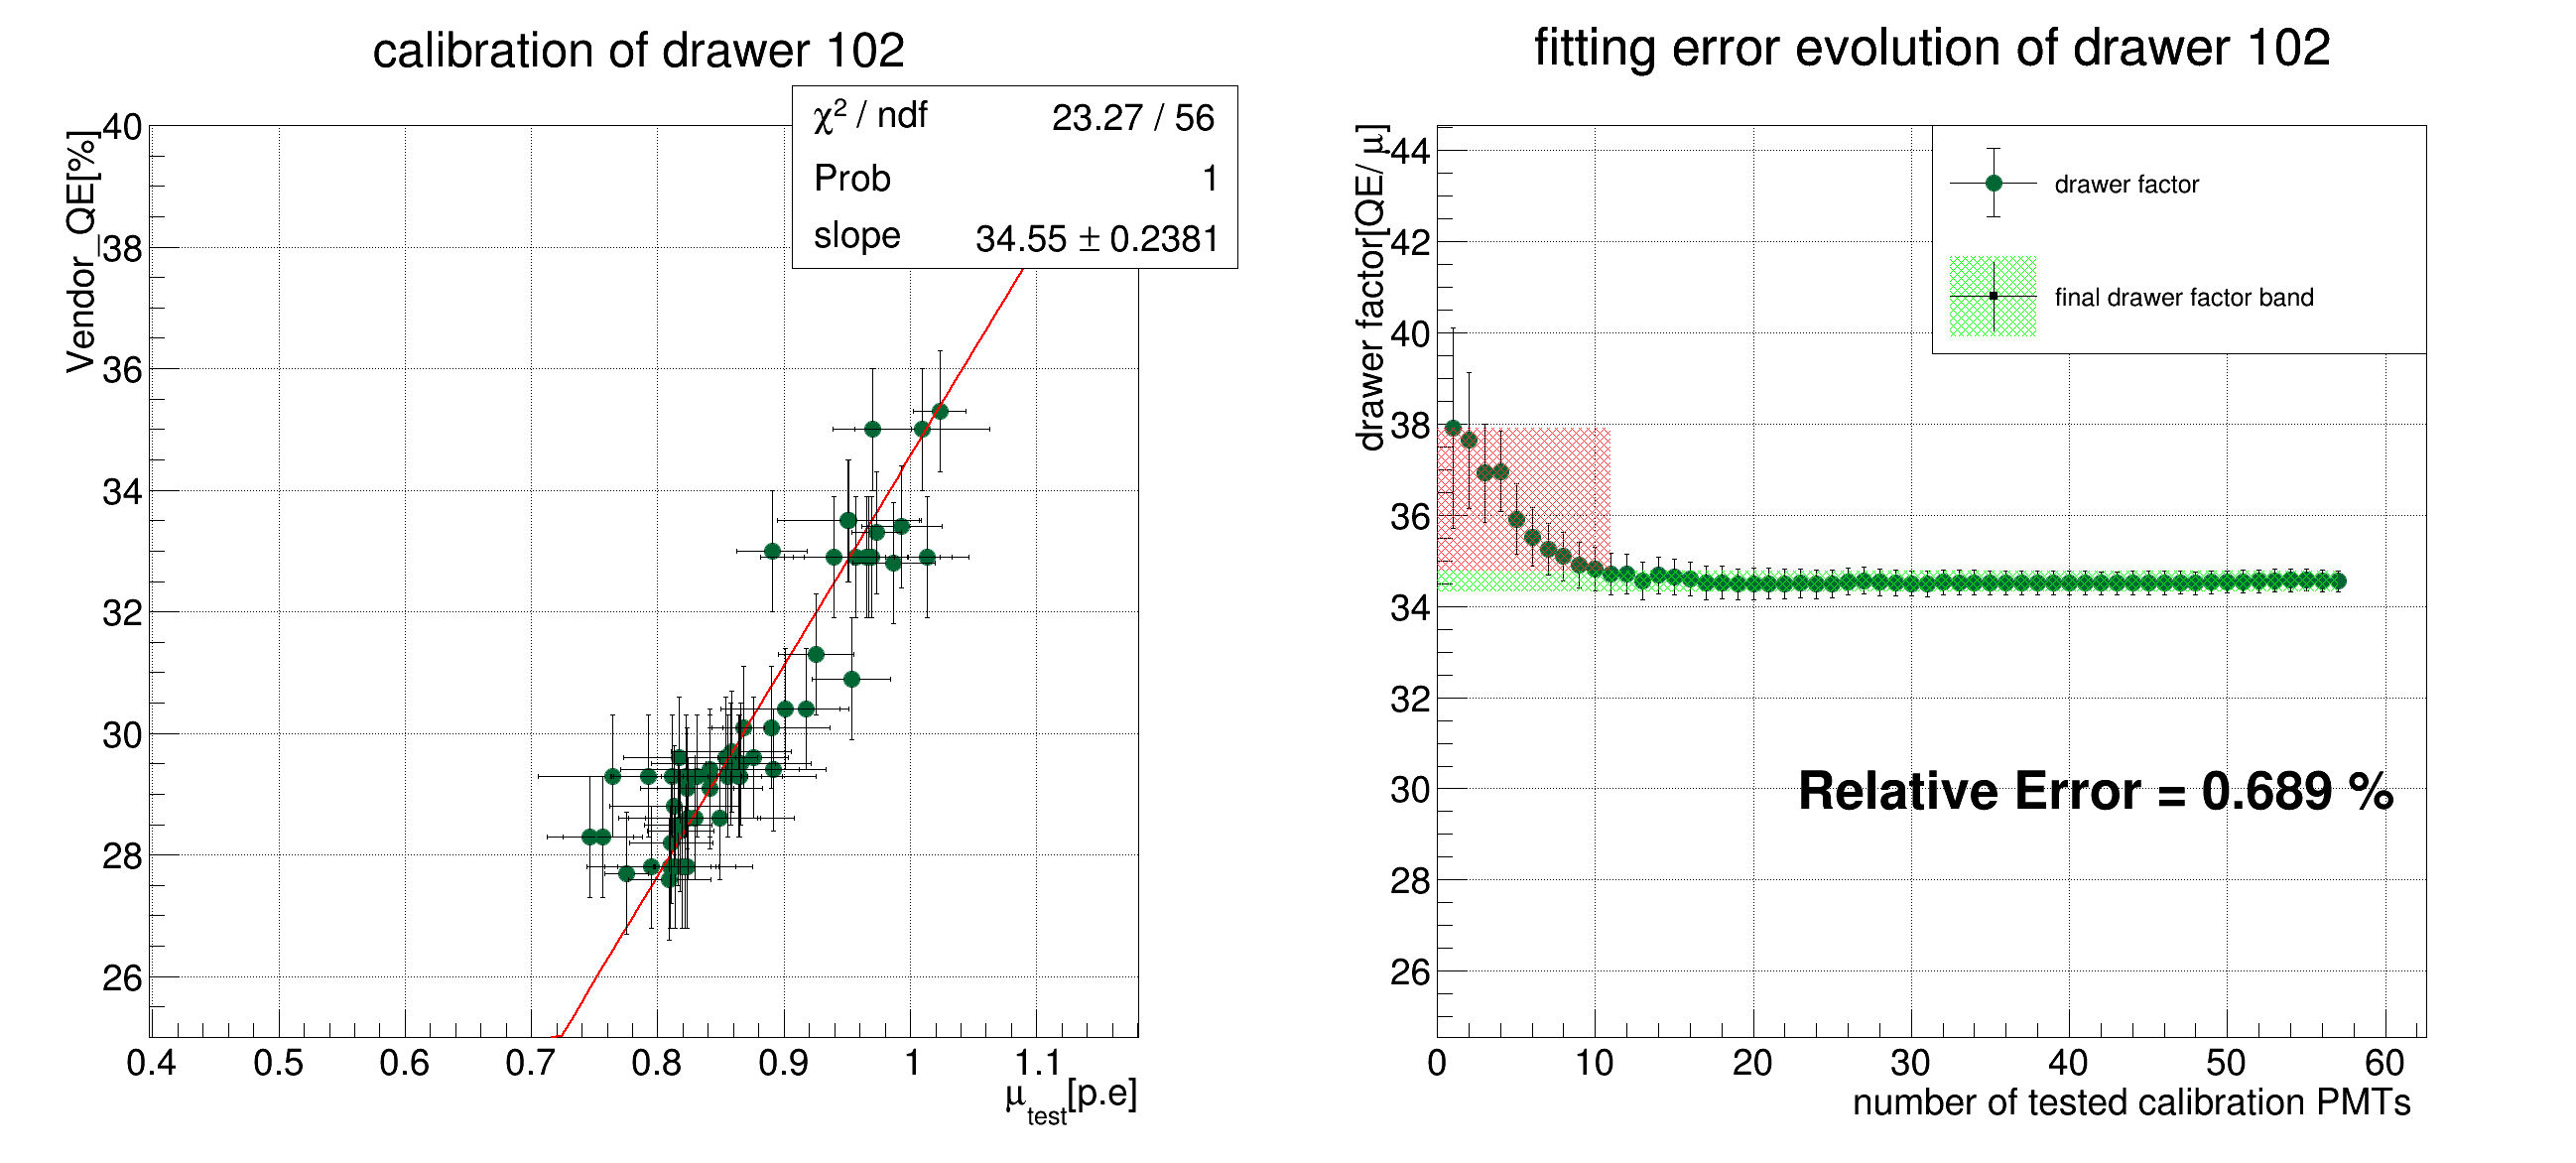
\includegraphics[width=0.45\textwidth]{sta101-1} 
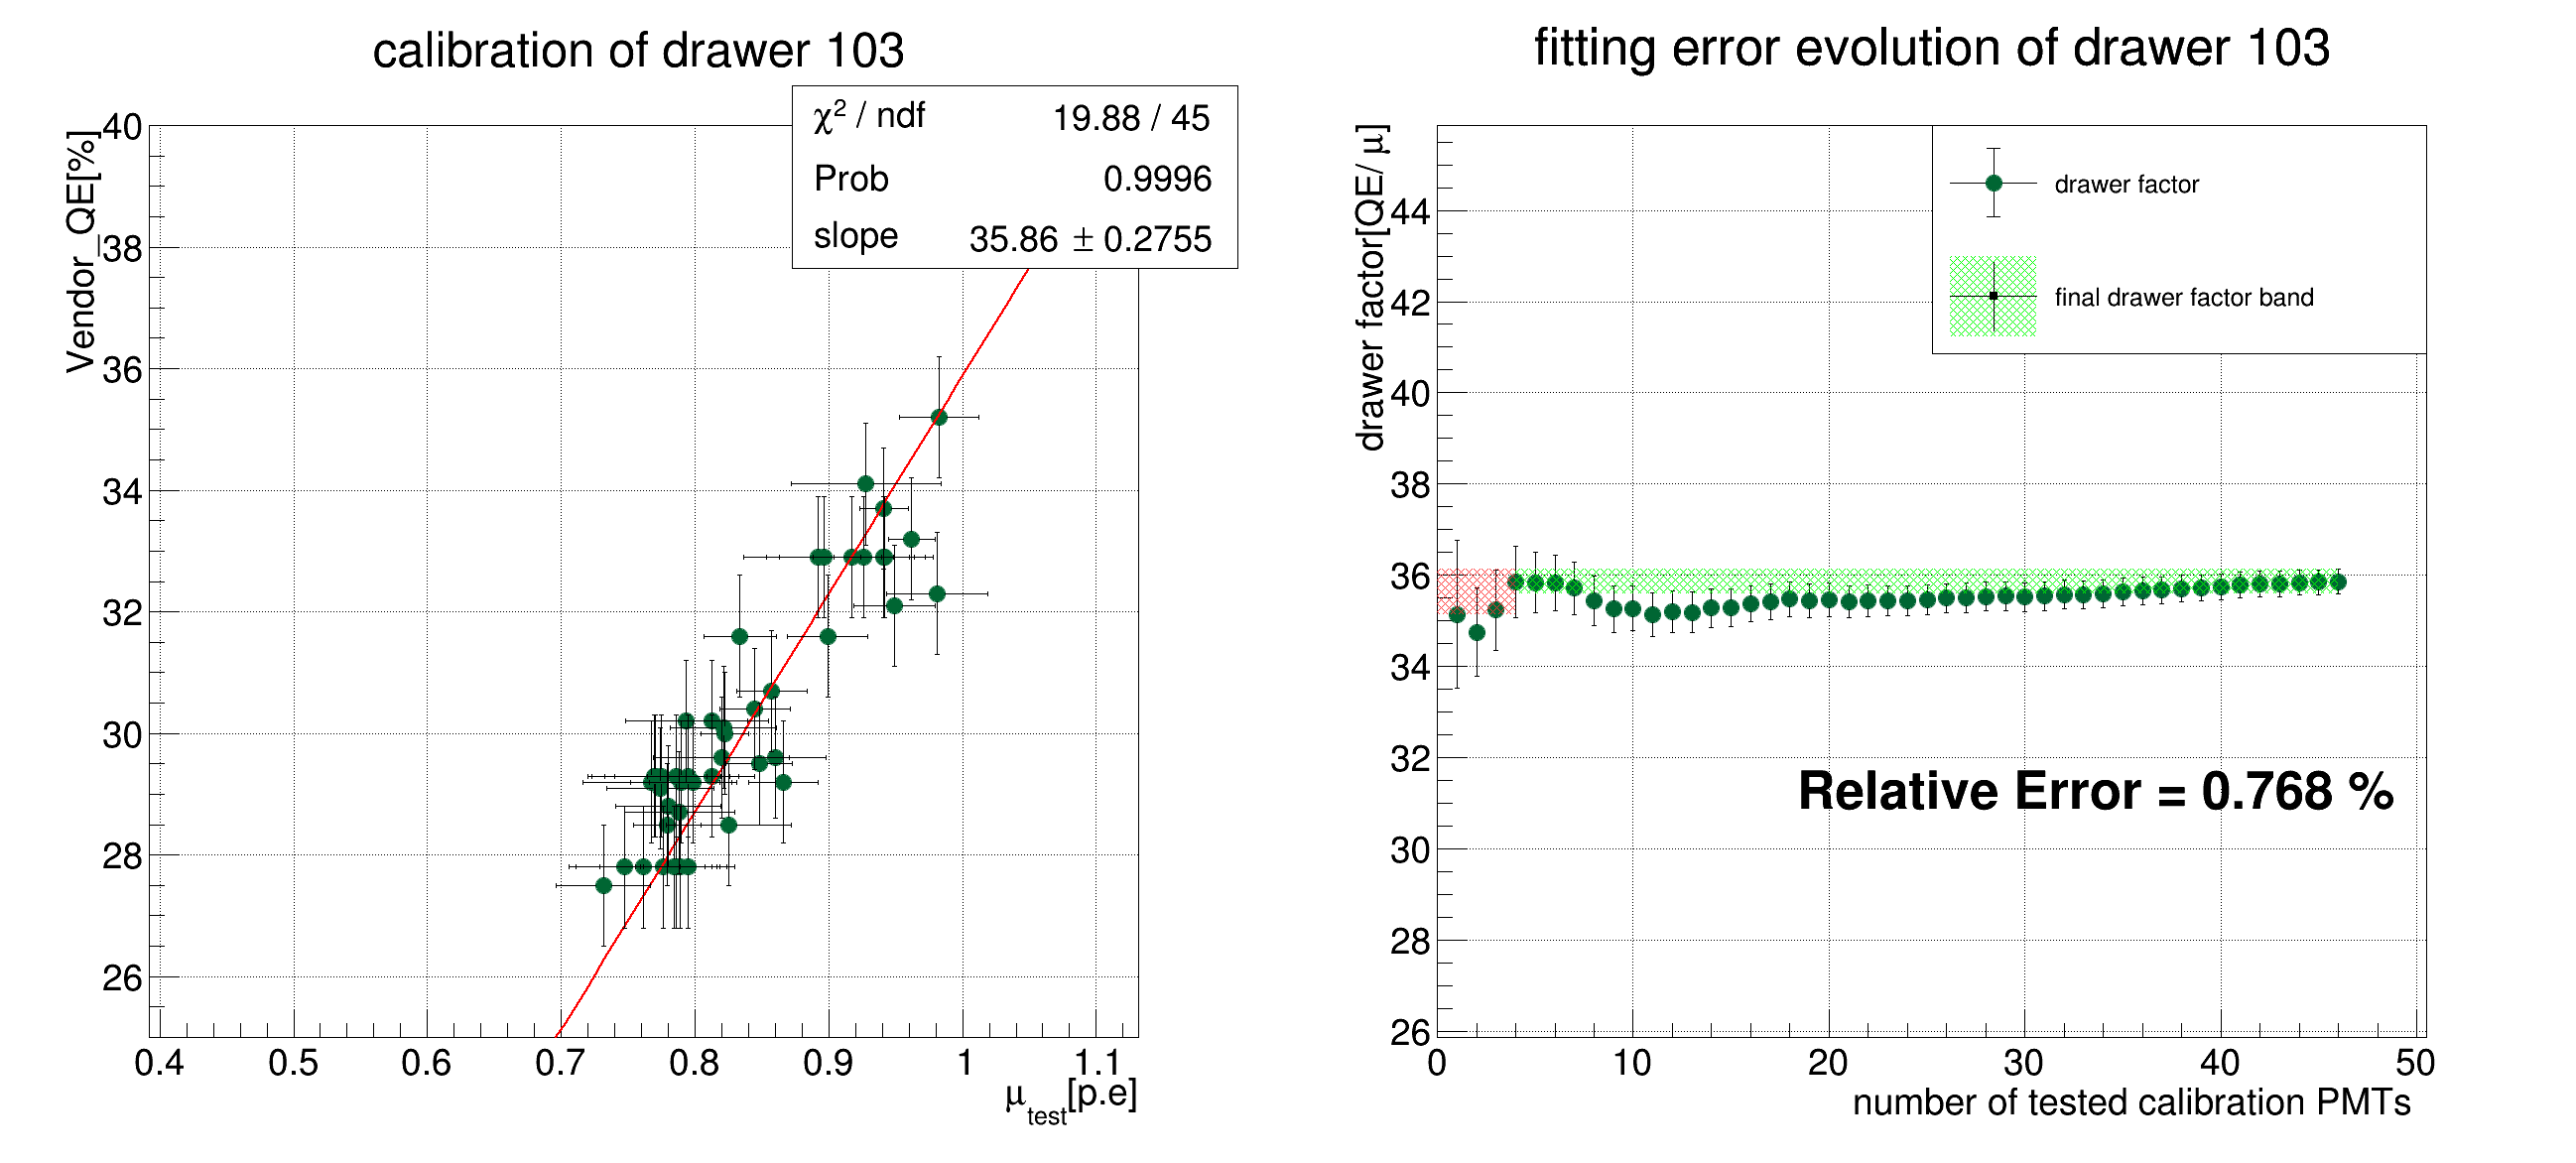
\includegraphics[width=0.45\textwidth]{sta101-2} 
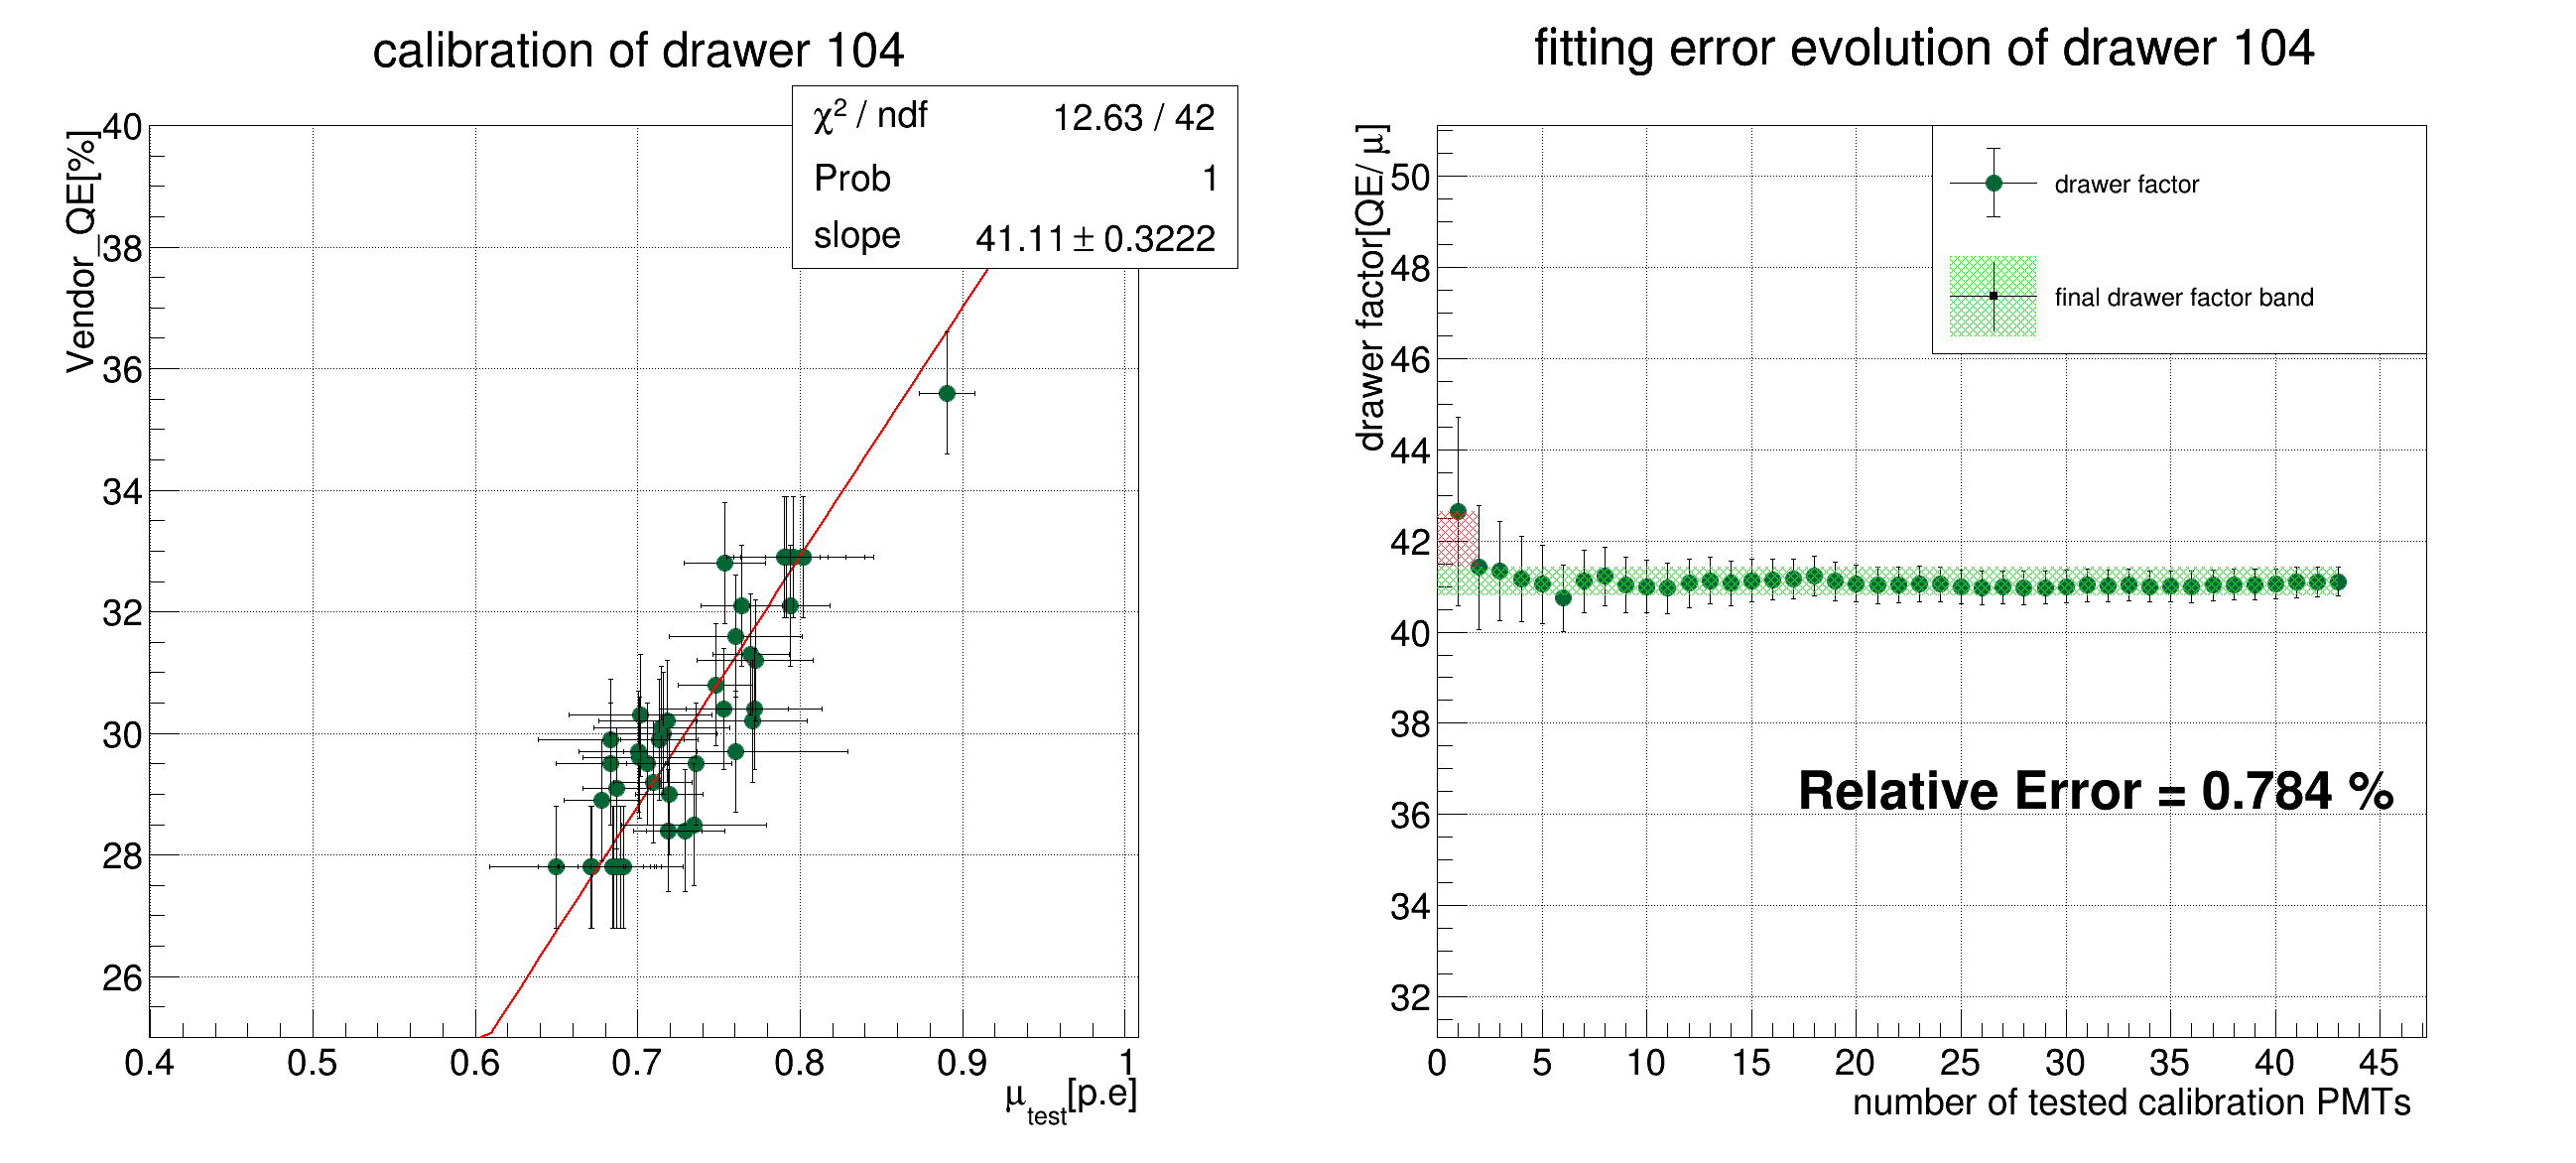
\includegraphics[width=0.45\textwidth]{sta101-3} 
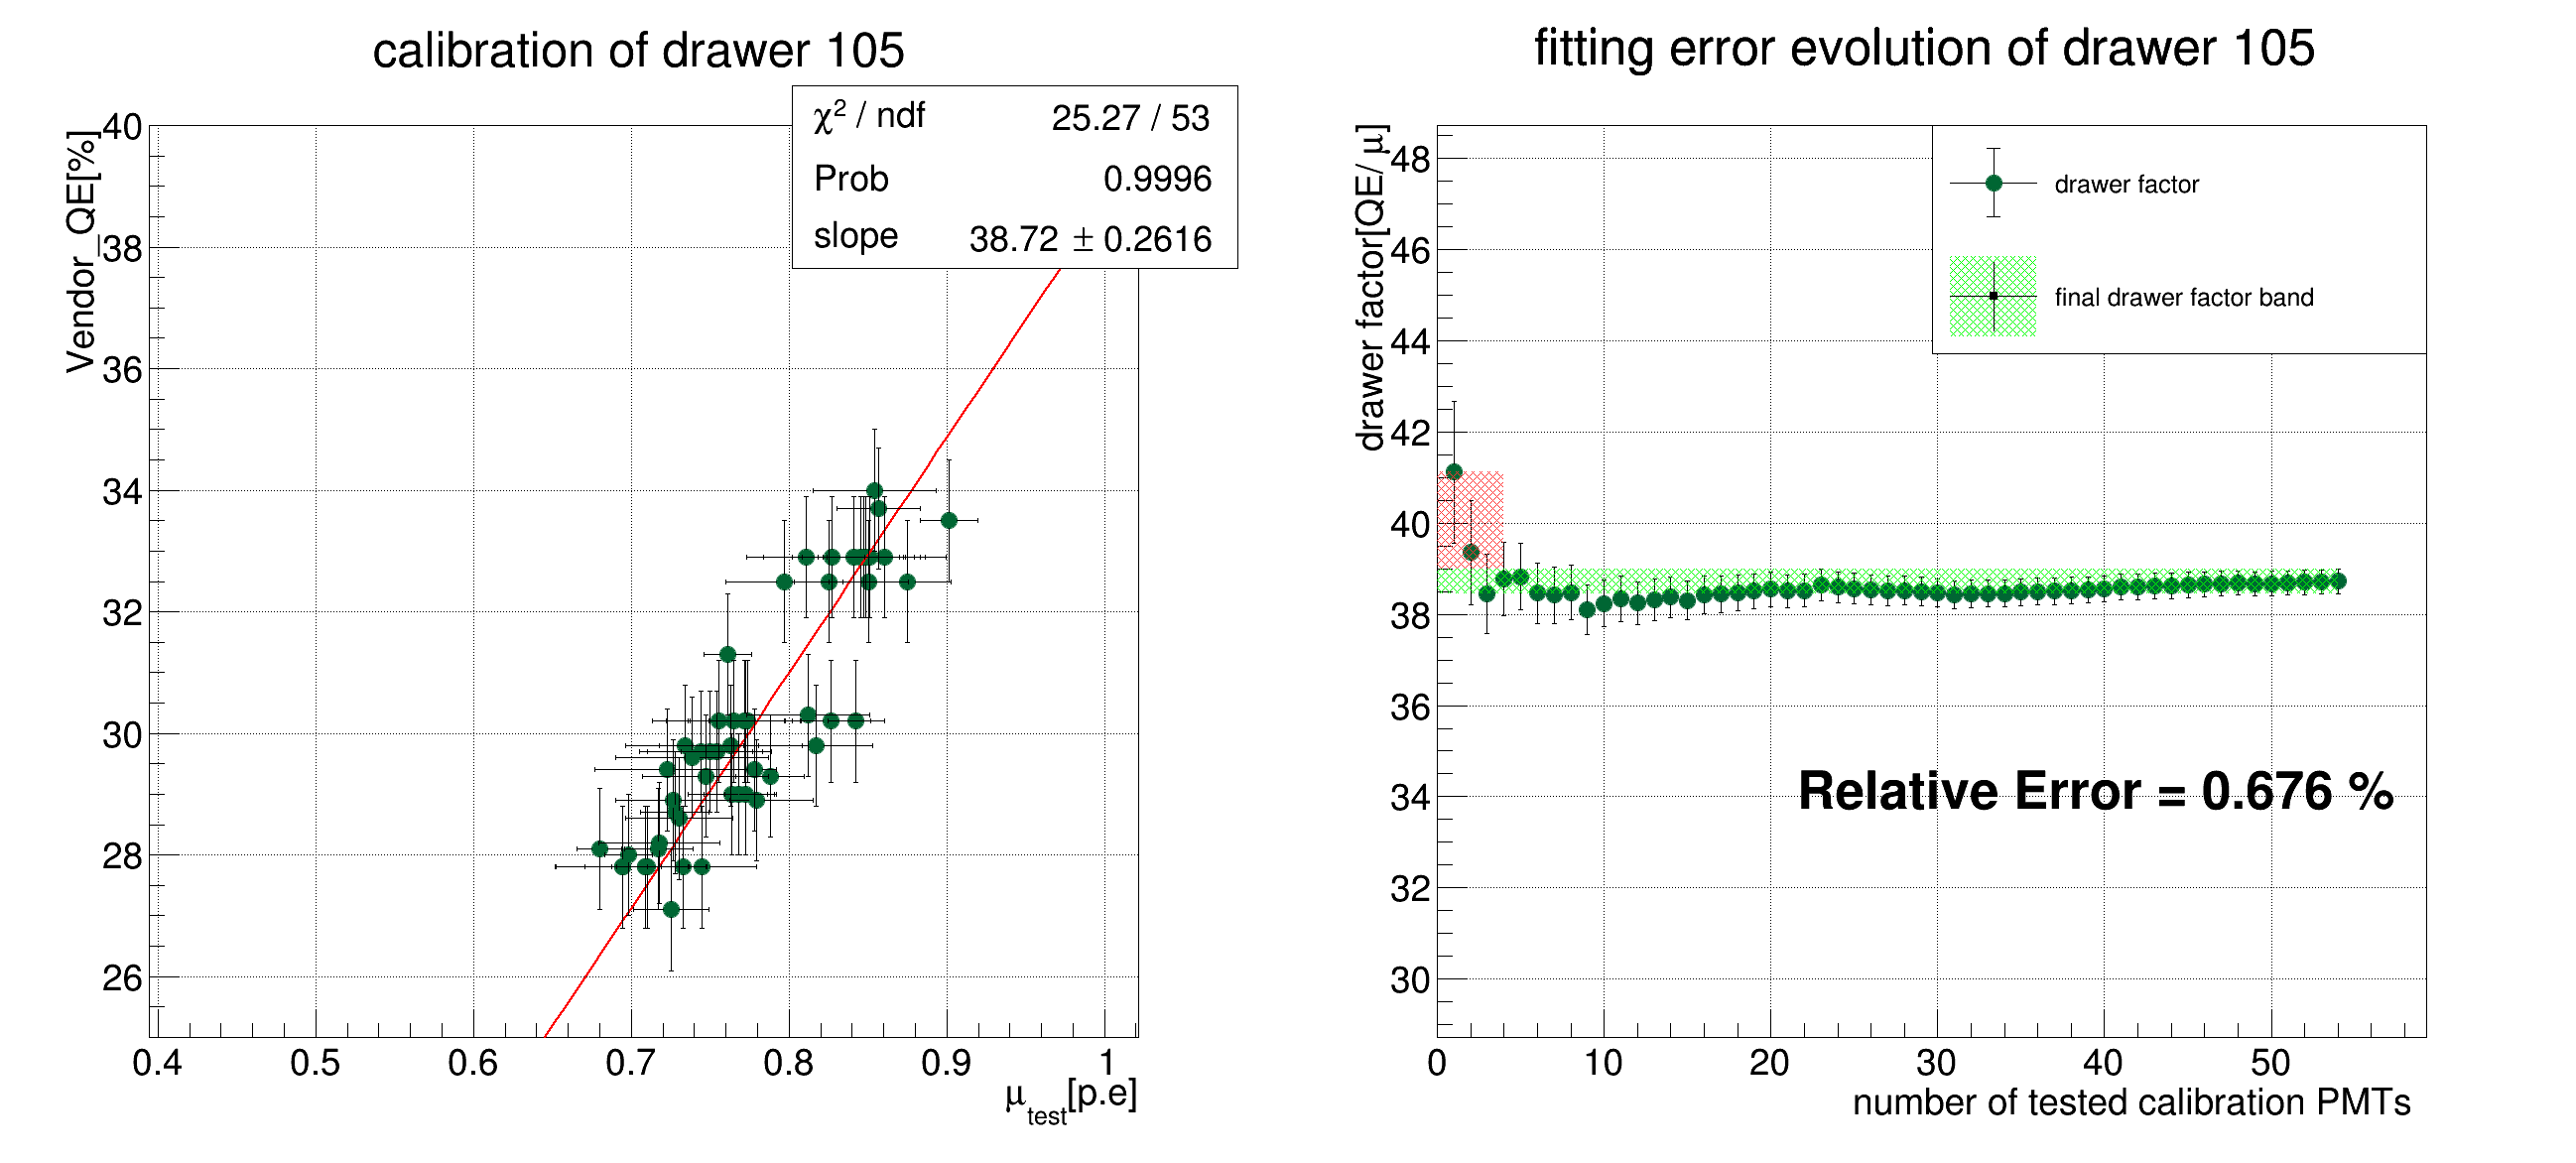
\includegraphics[width=0.45\textwidth]{sta101-4} 
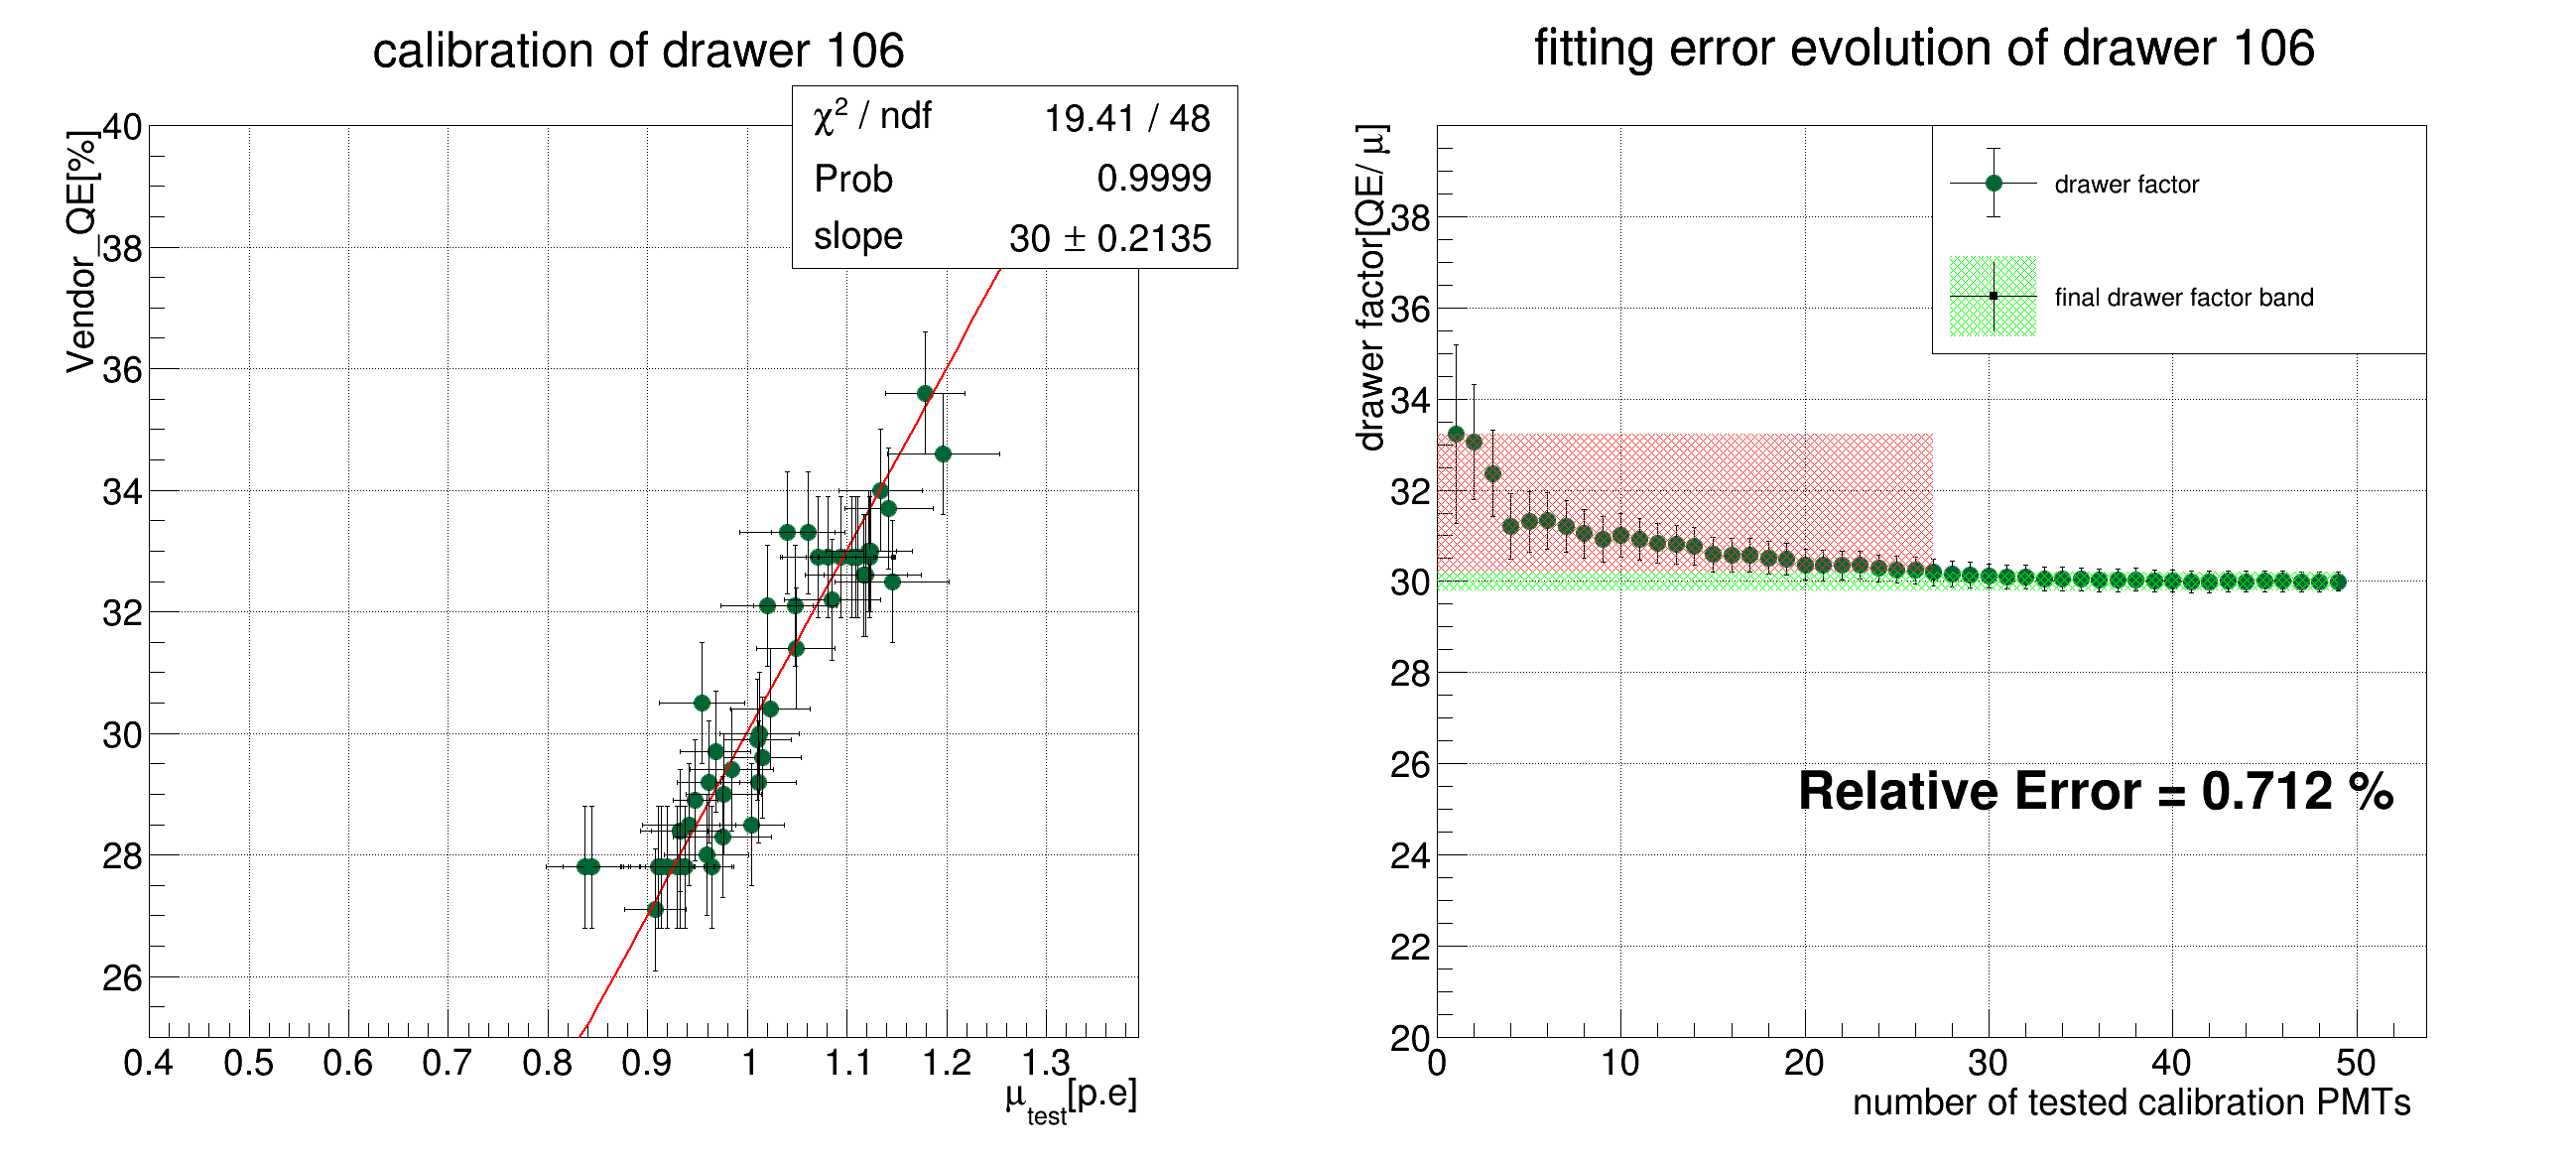
\includegraphics[width=0.45\textwidth]{sta101-5} 
\end{frame}
\begin{frame}{drawer-calibration}
\vspace{-.5cm}
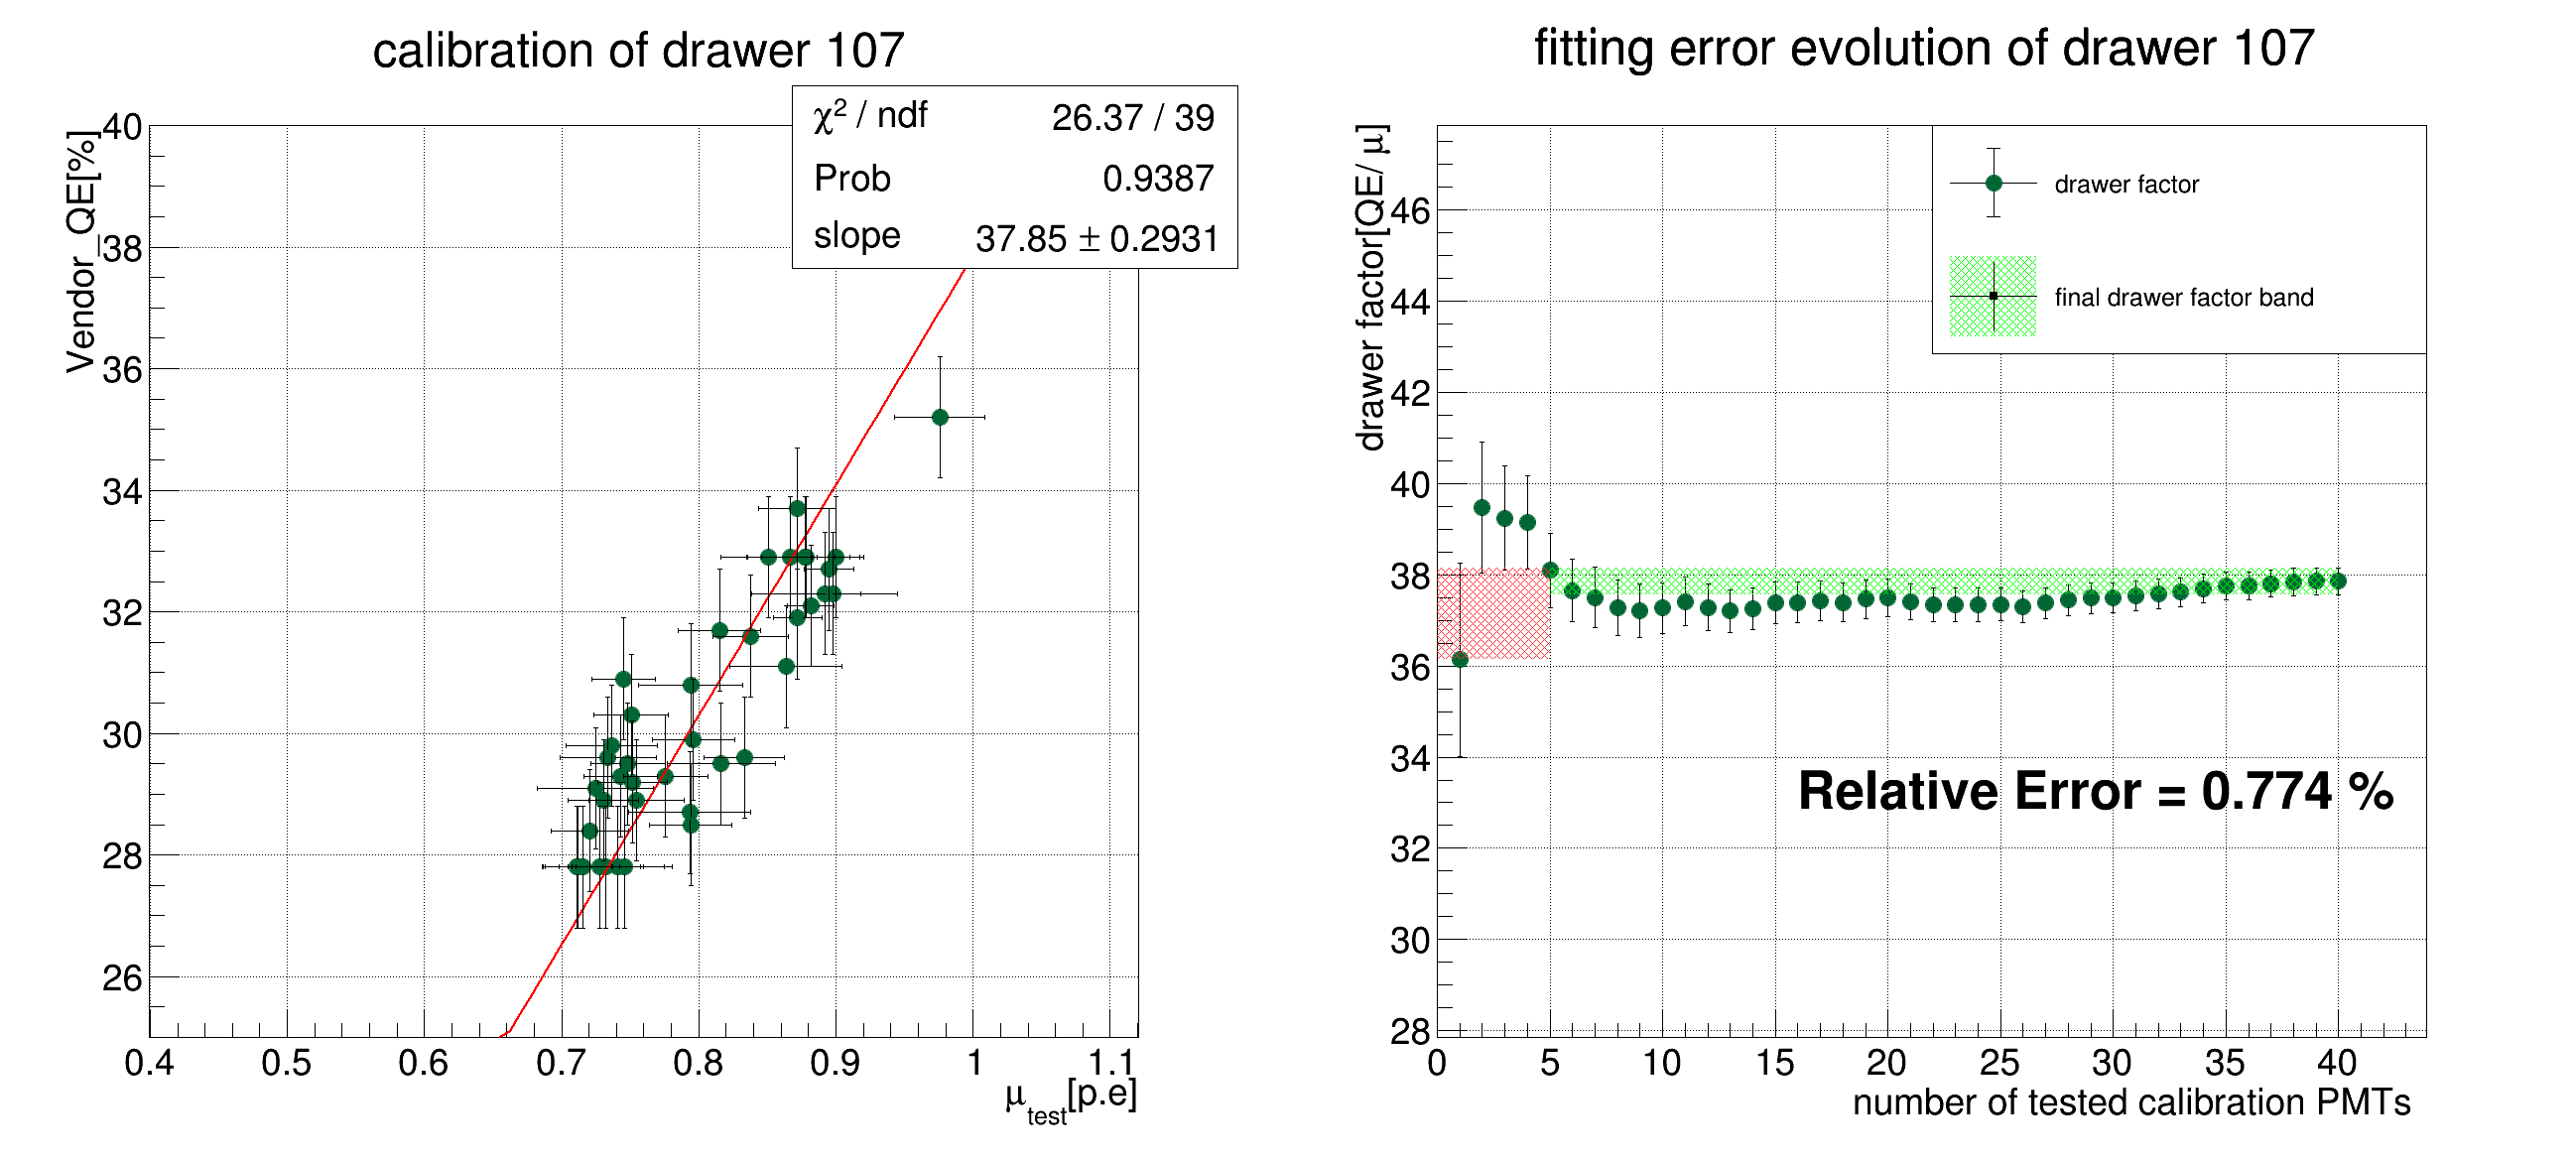
\includegraphics[width=0.45\textwidth]{sta101-6} 
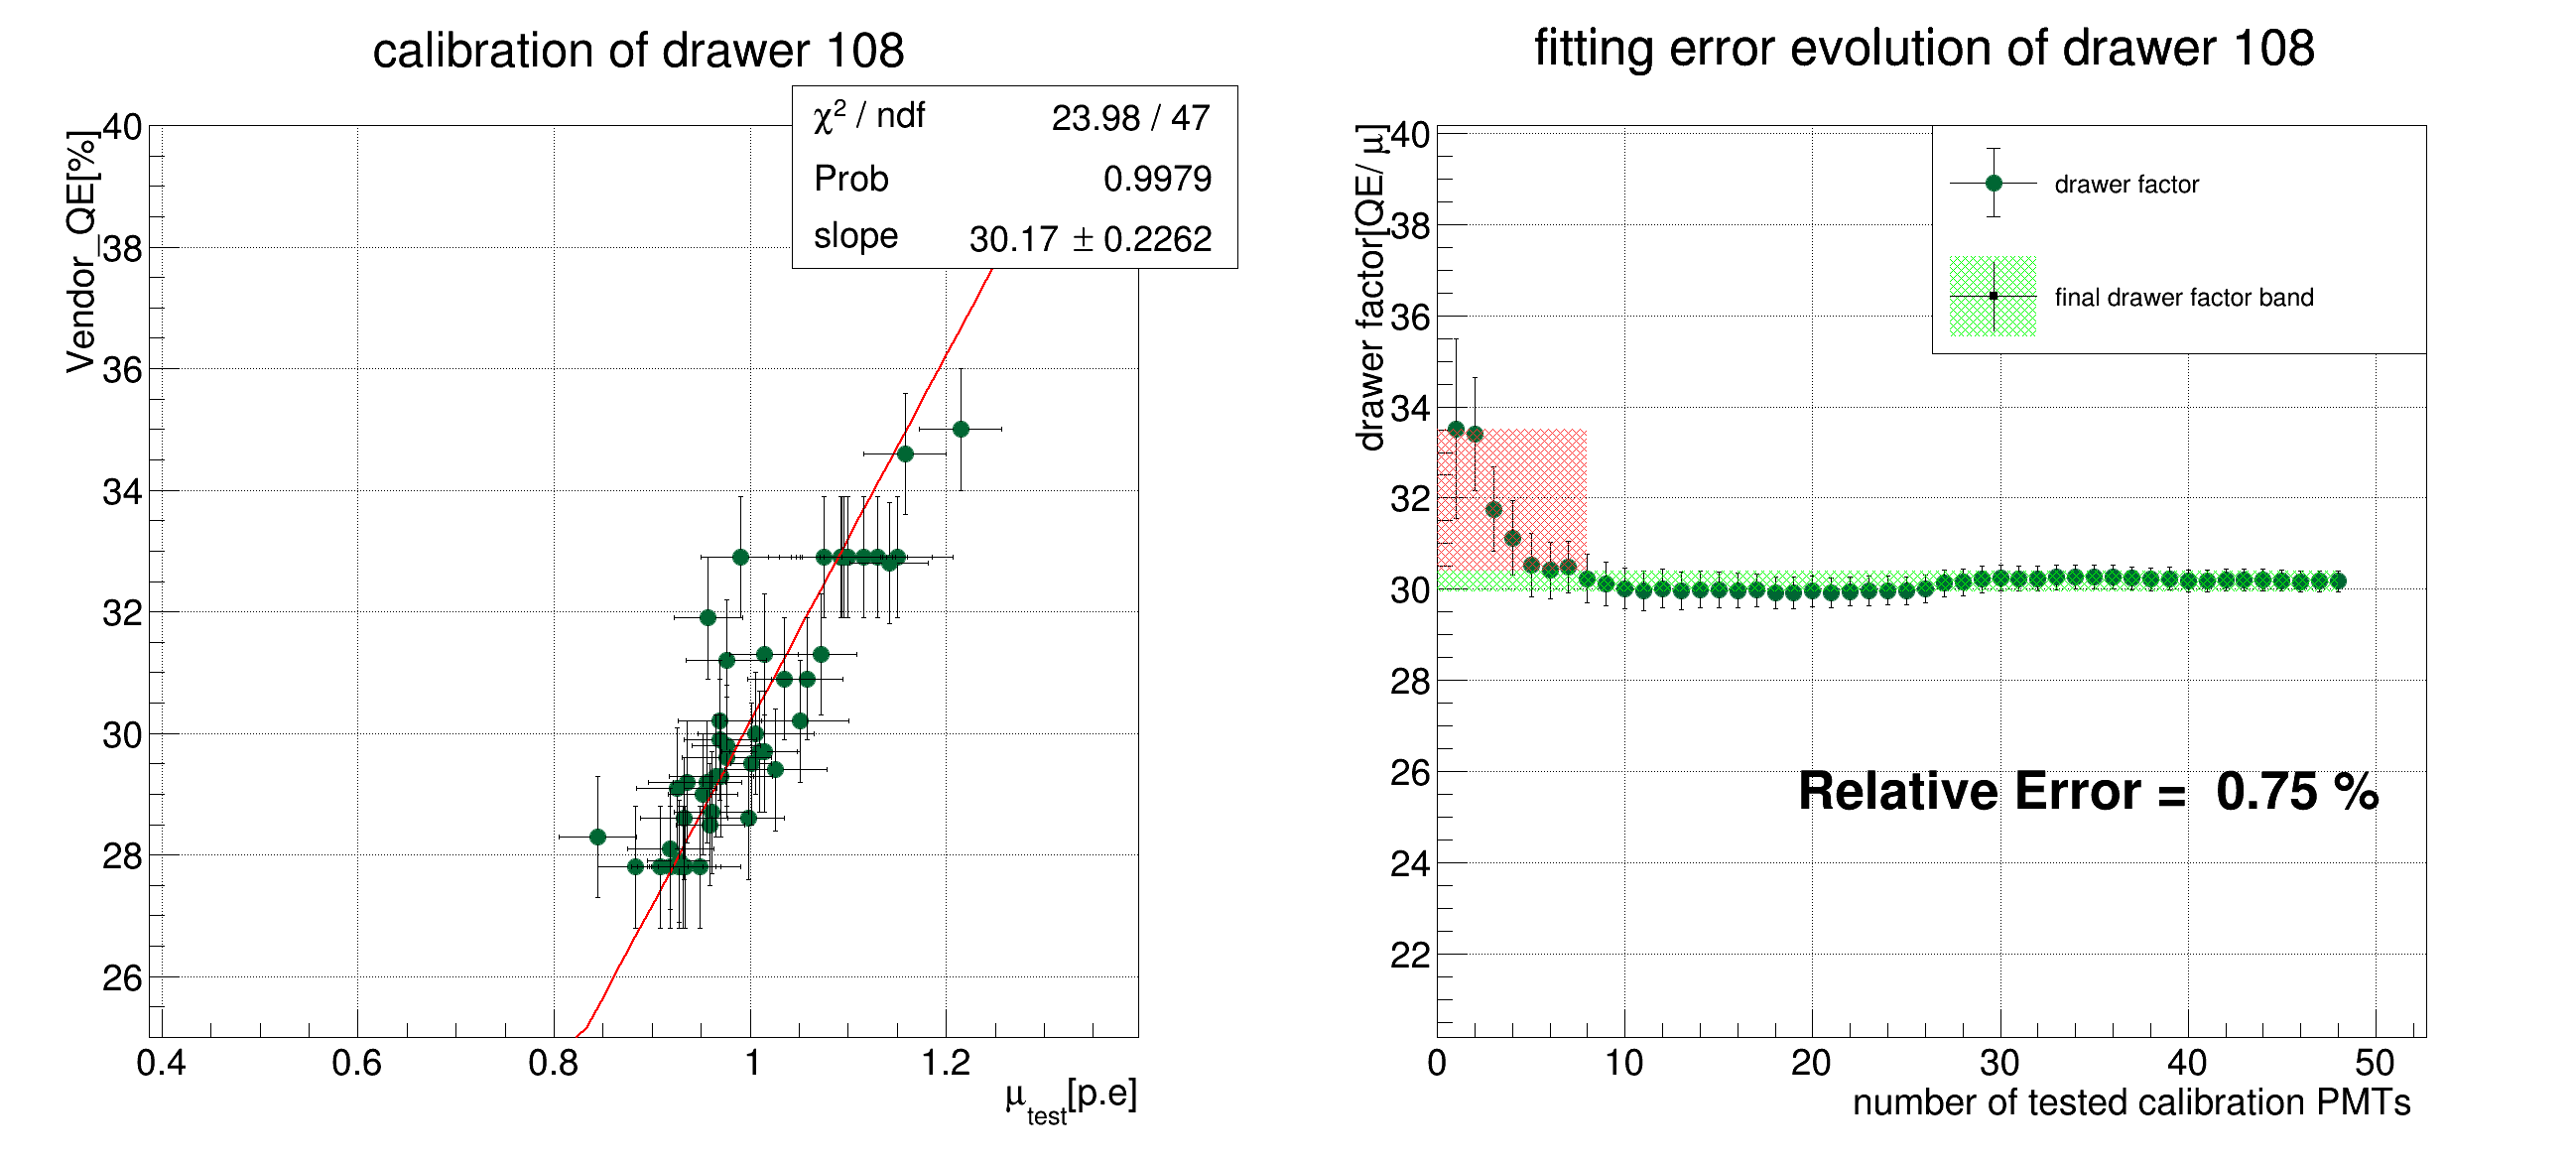
\includegraphics[width=0.45\textwidth]{sta101-7} 
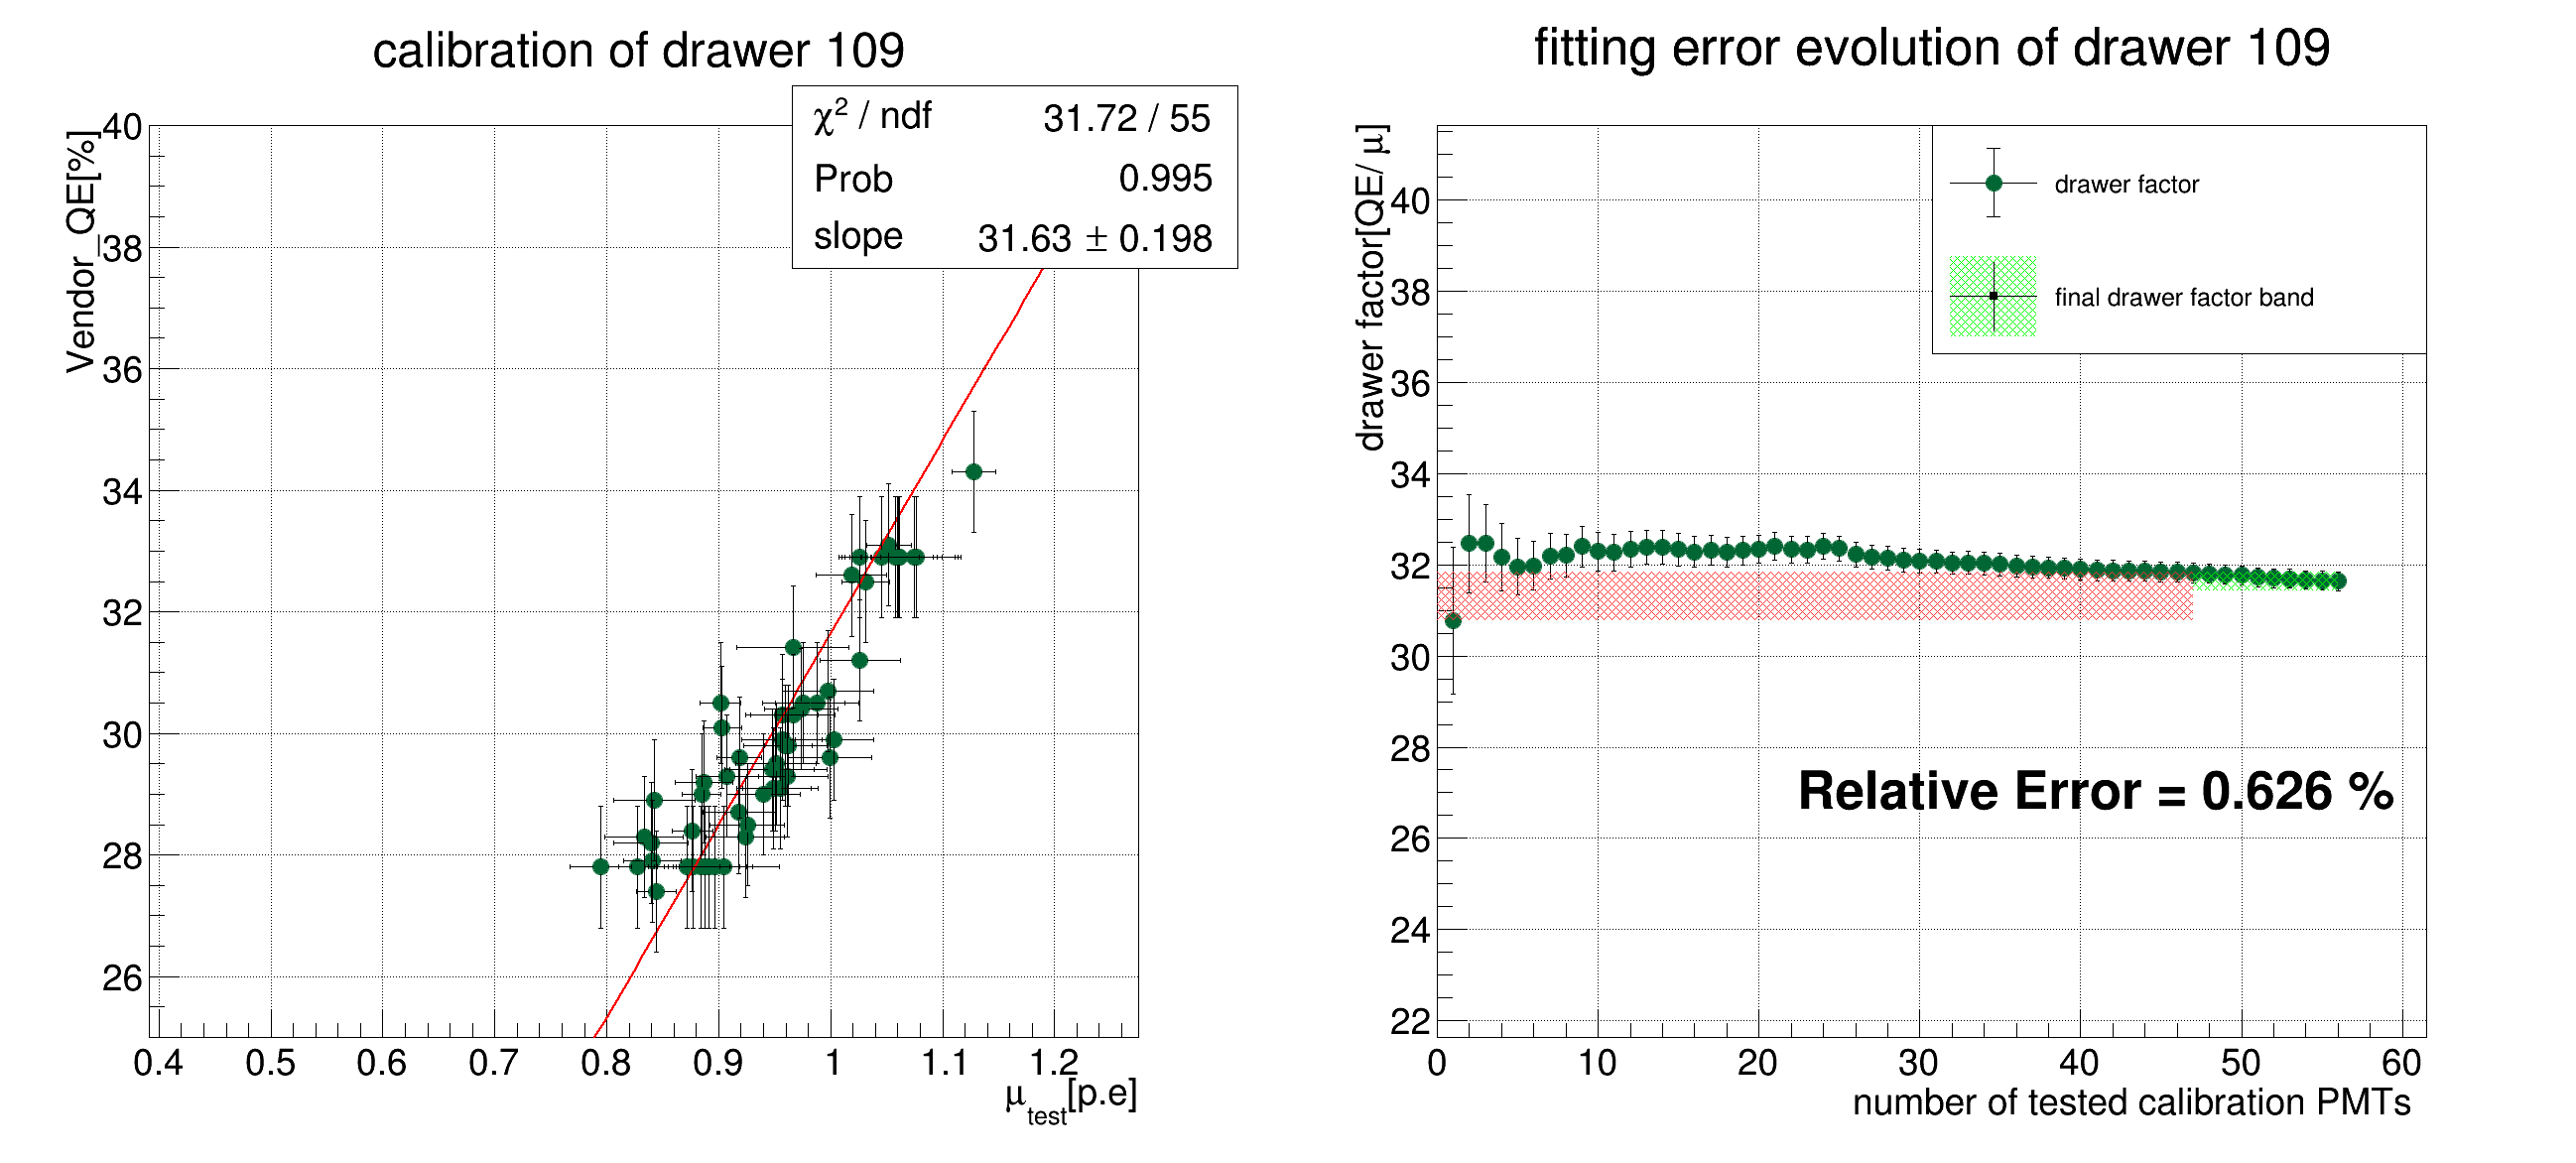
\includegraphics[width=0.45\textwidth]{sta101-8} 
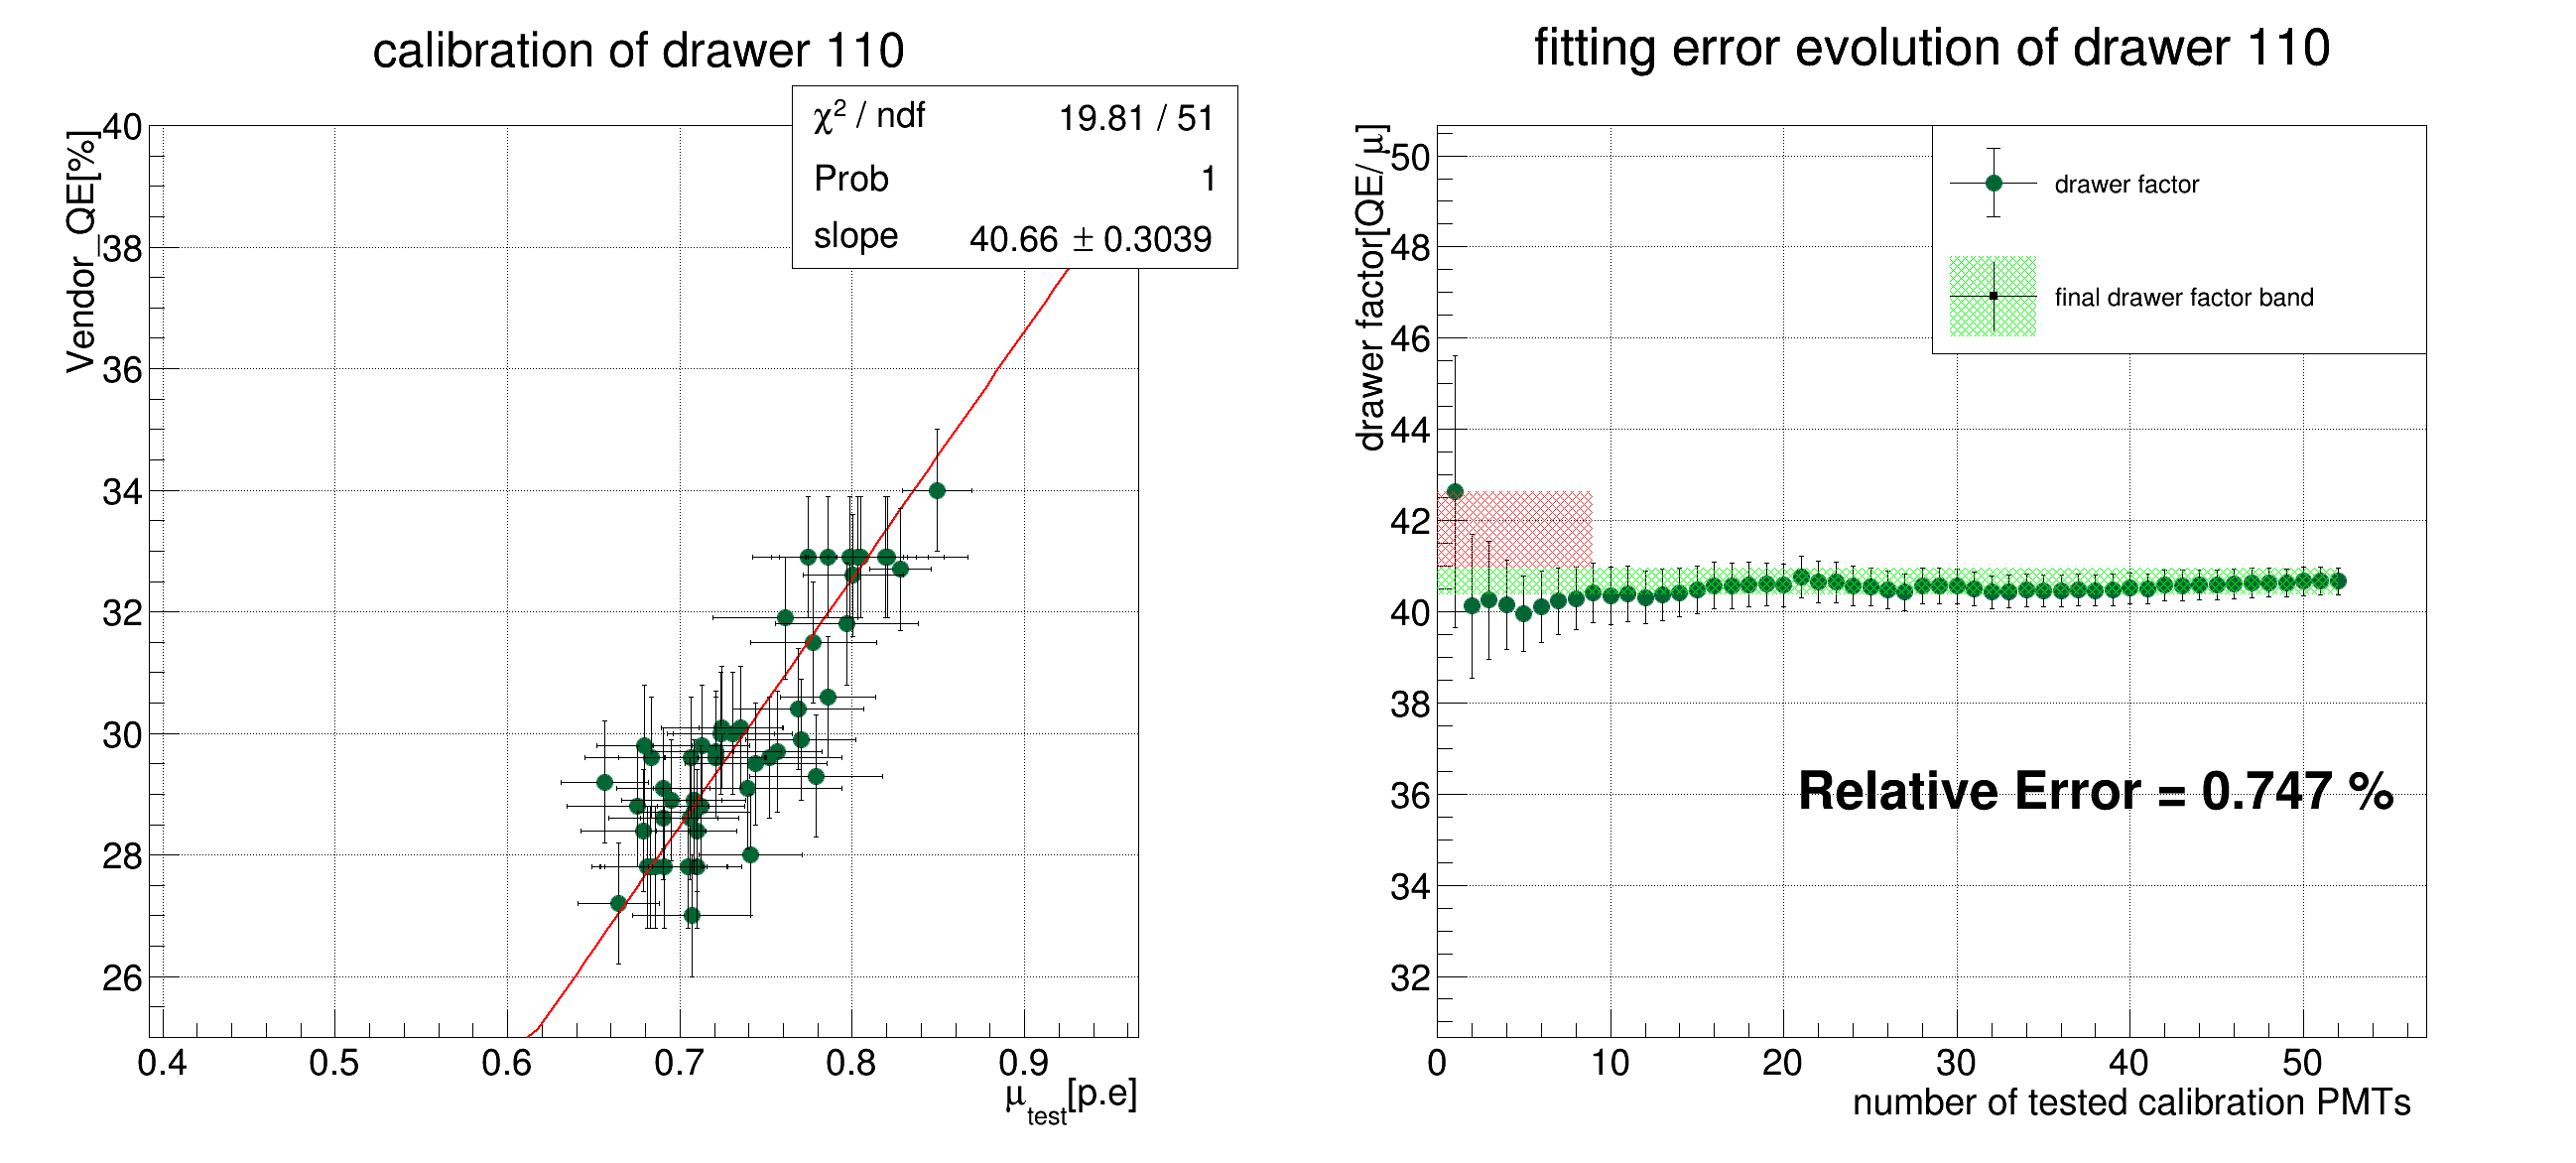
\includegraphics[width=0.45\textwidth]{sta101-9} 
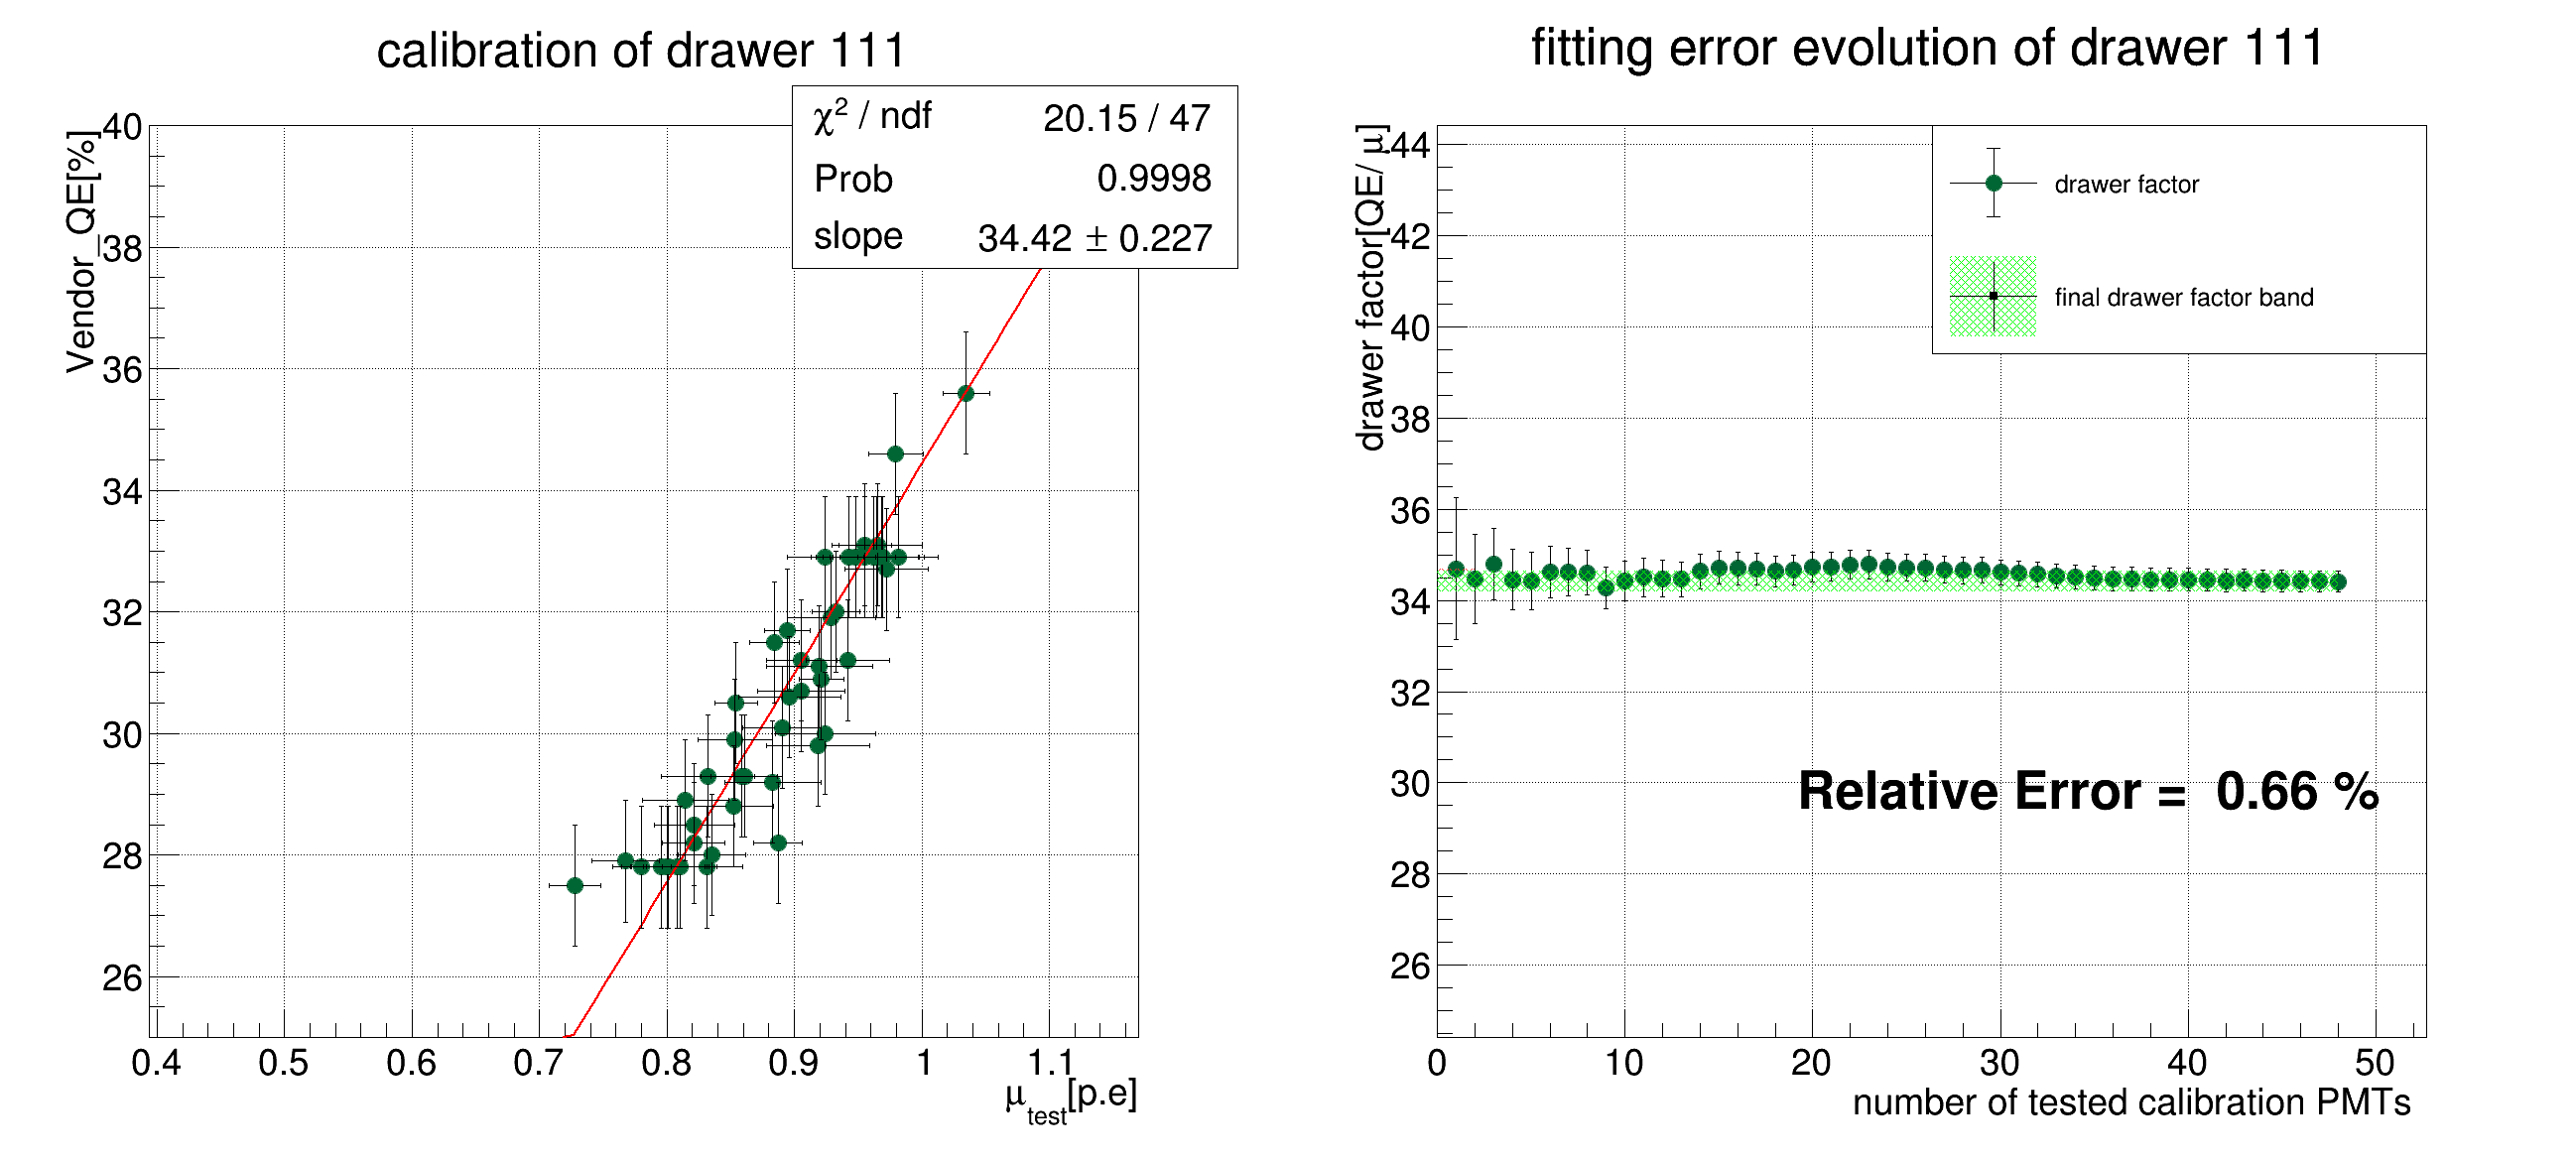
\includegraphics[width=0.45\textwidth]{sta101-10} 
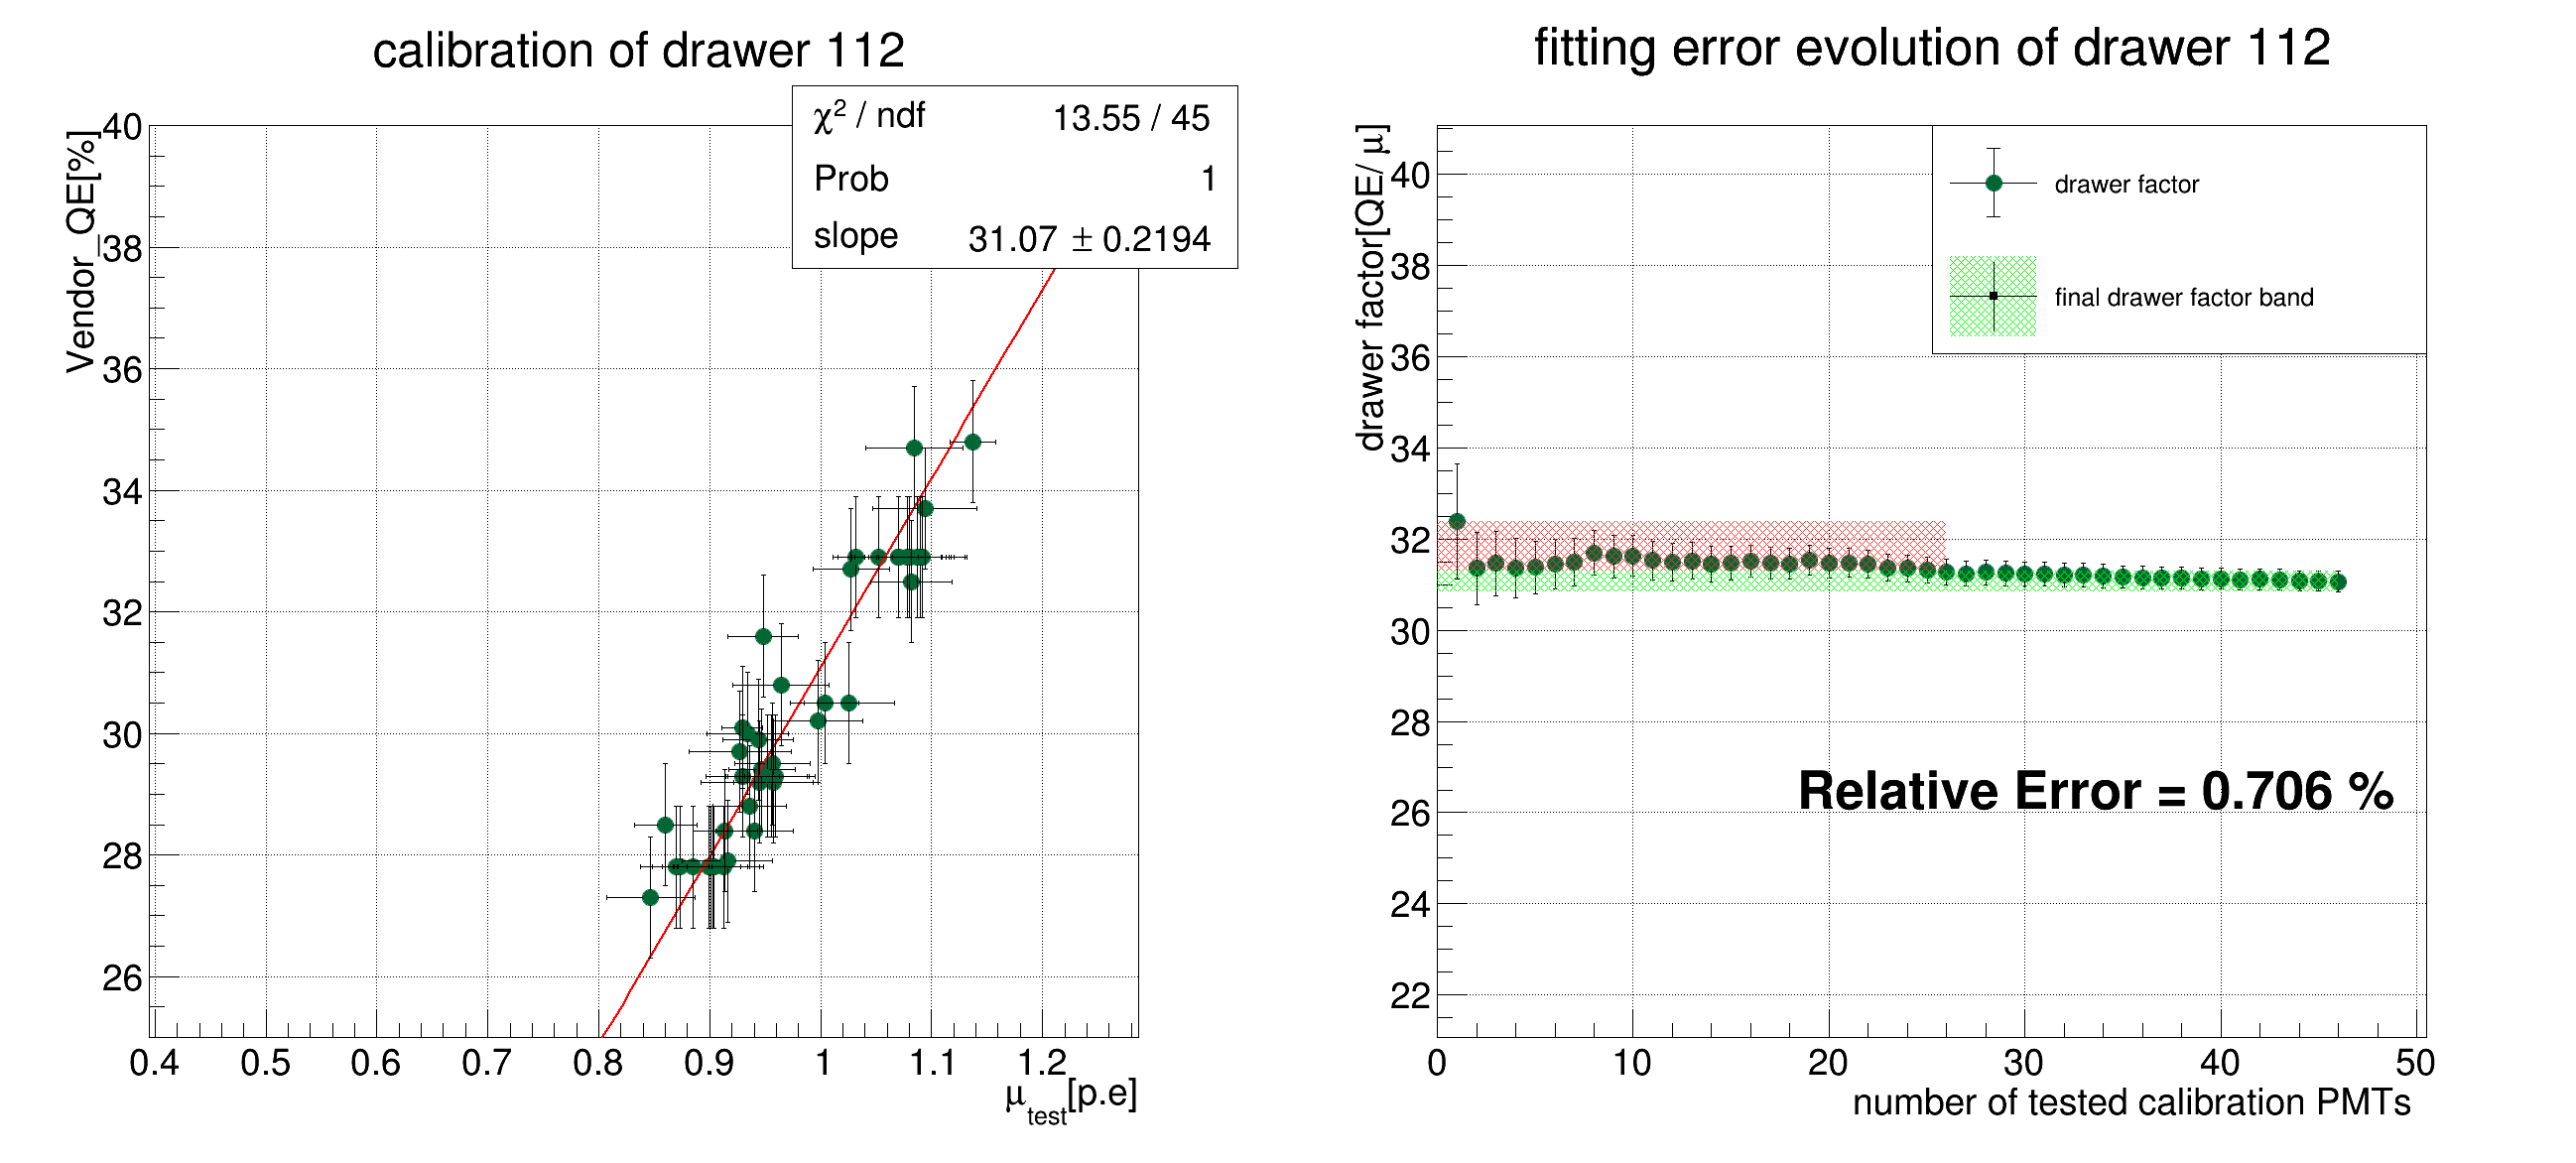
\includegraphics[width=0.45\textwidth]{sta101-11} 
\end{frame}
\begin{frame}{drawer-calibration}
\vspace{-.5cm}
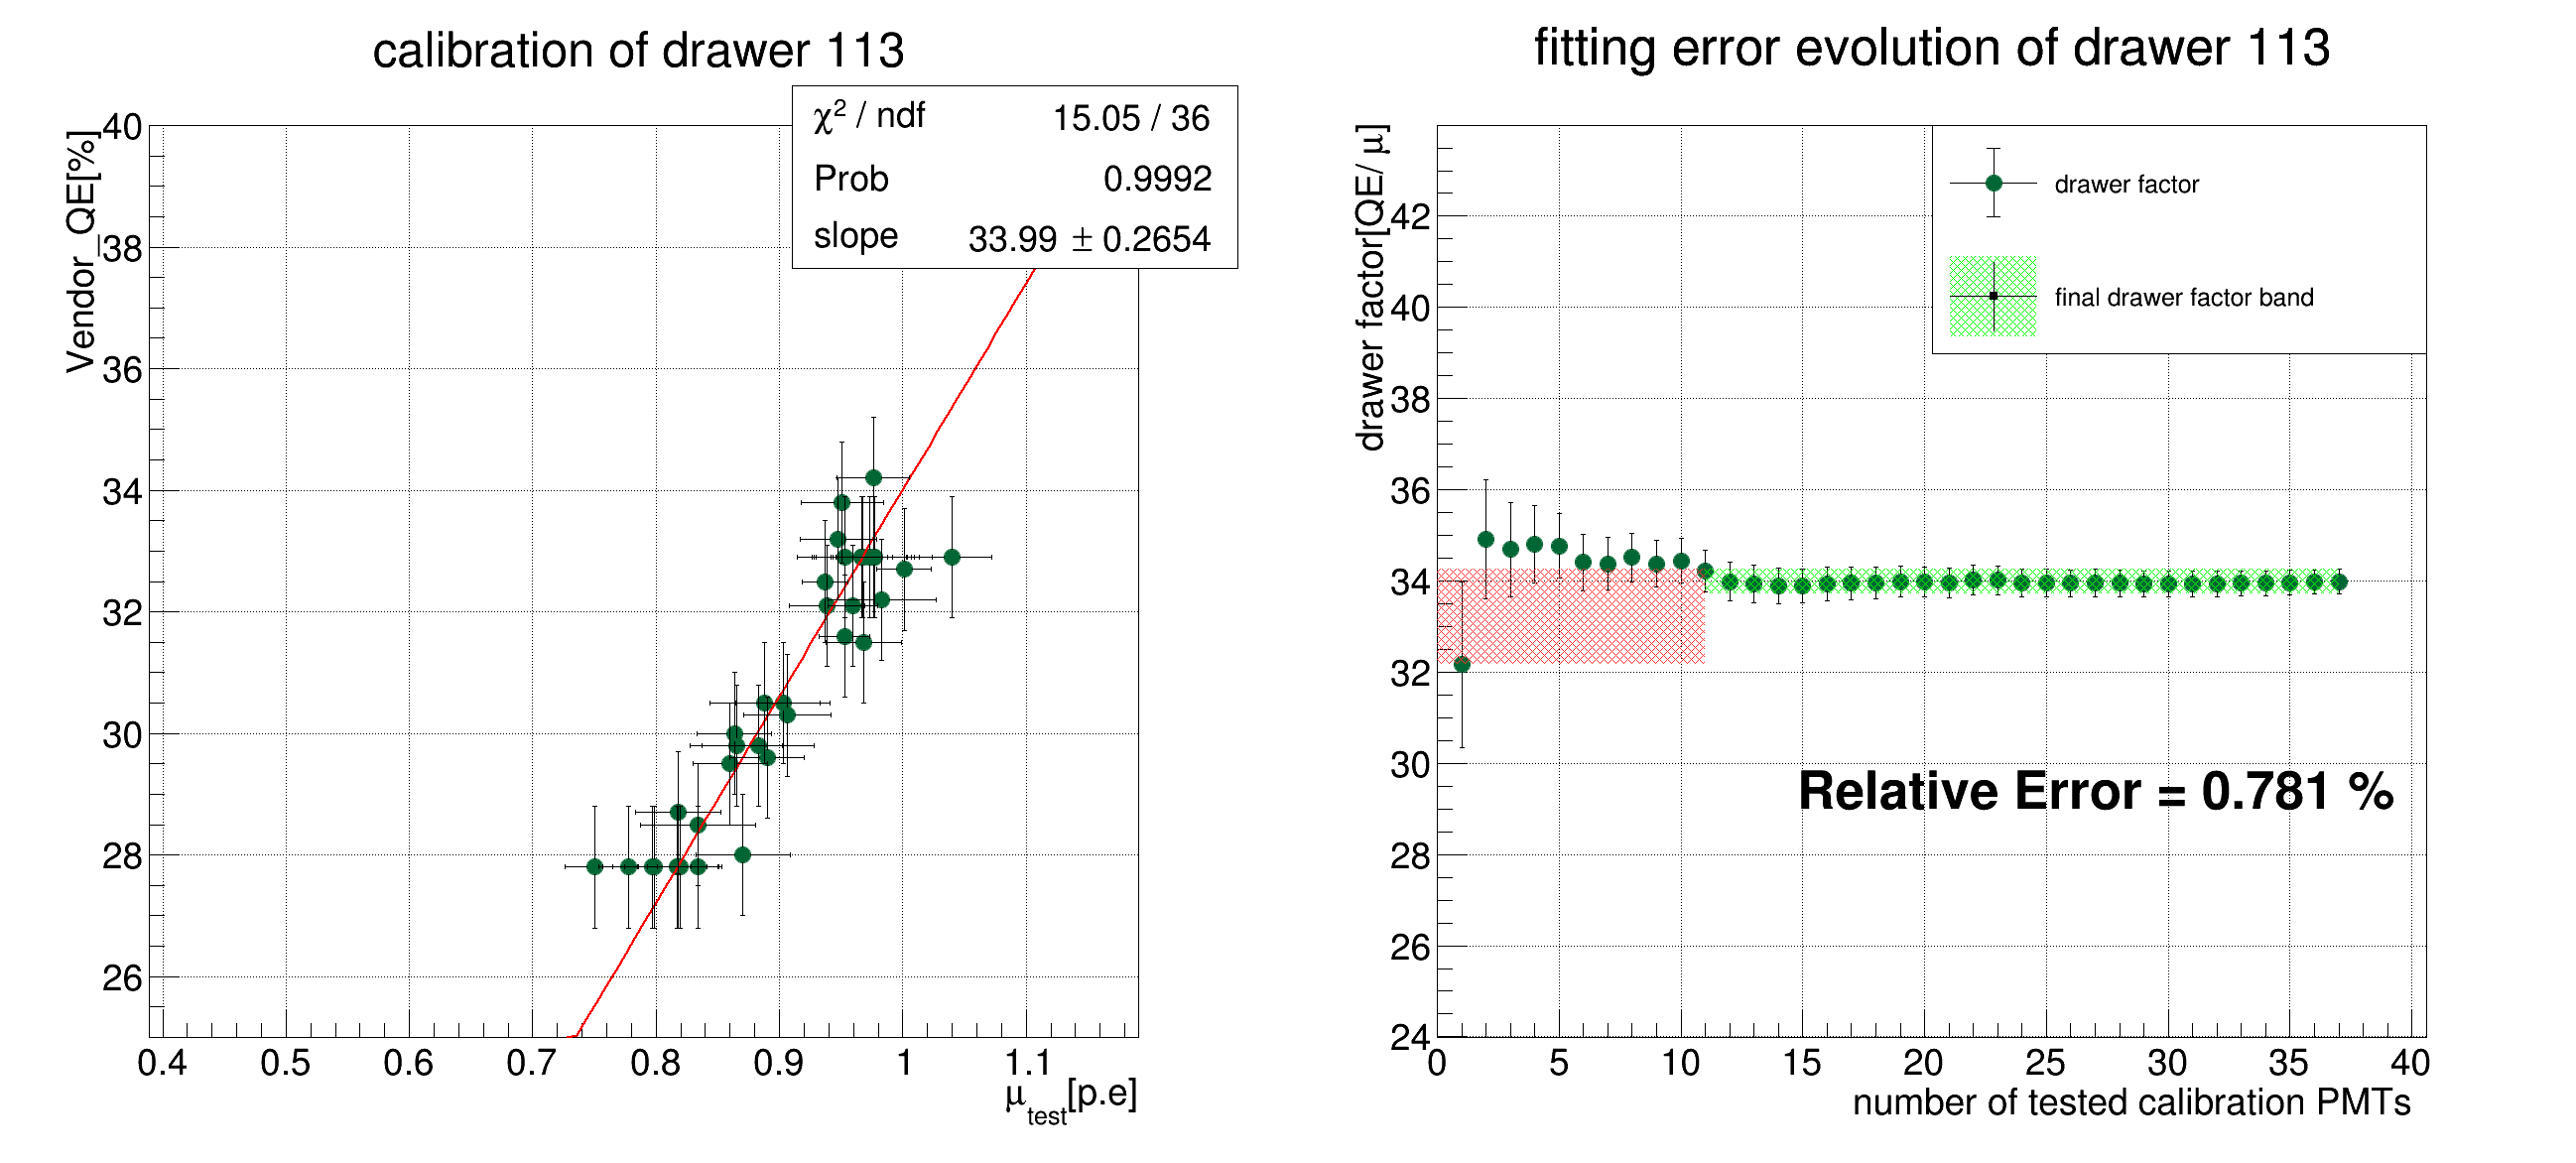
\includegraphics[width=0.45\textwidth]{sta101-12} 
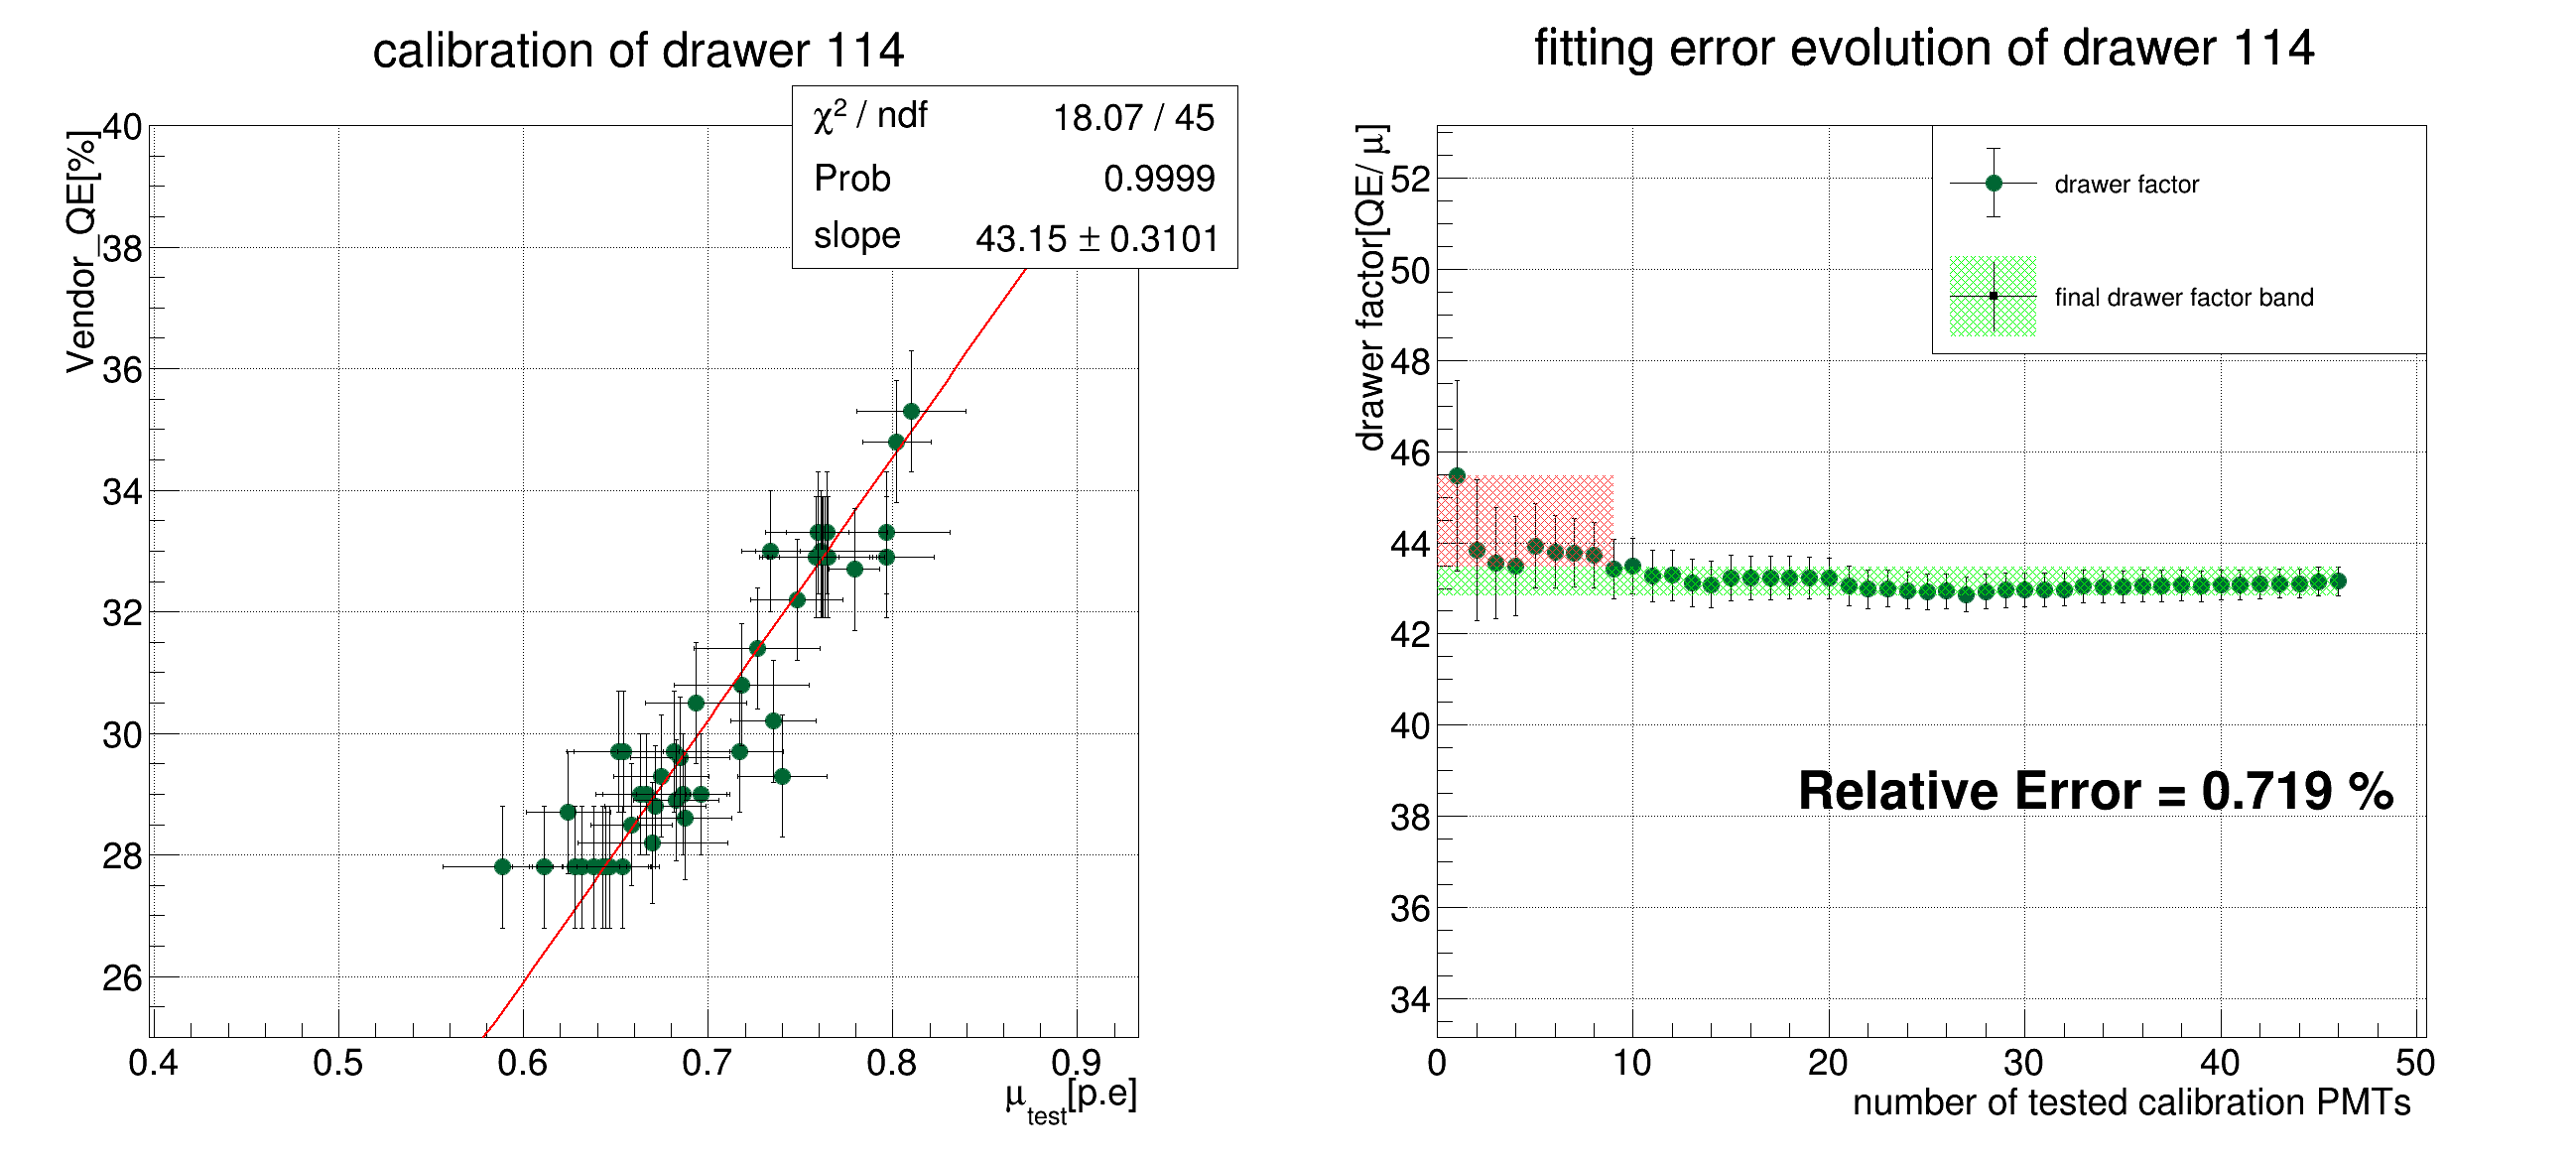
\includegraphics[width=0.45\textwidth]{sta101-13} 
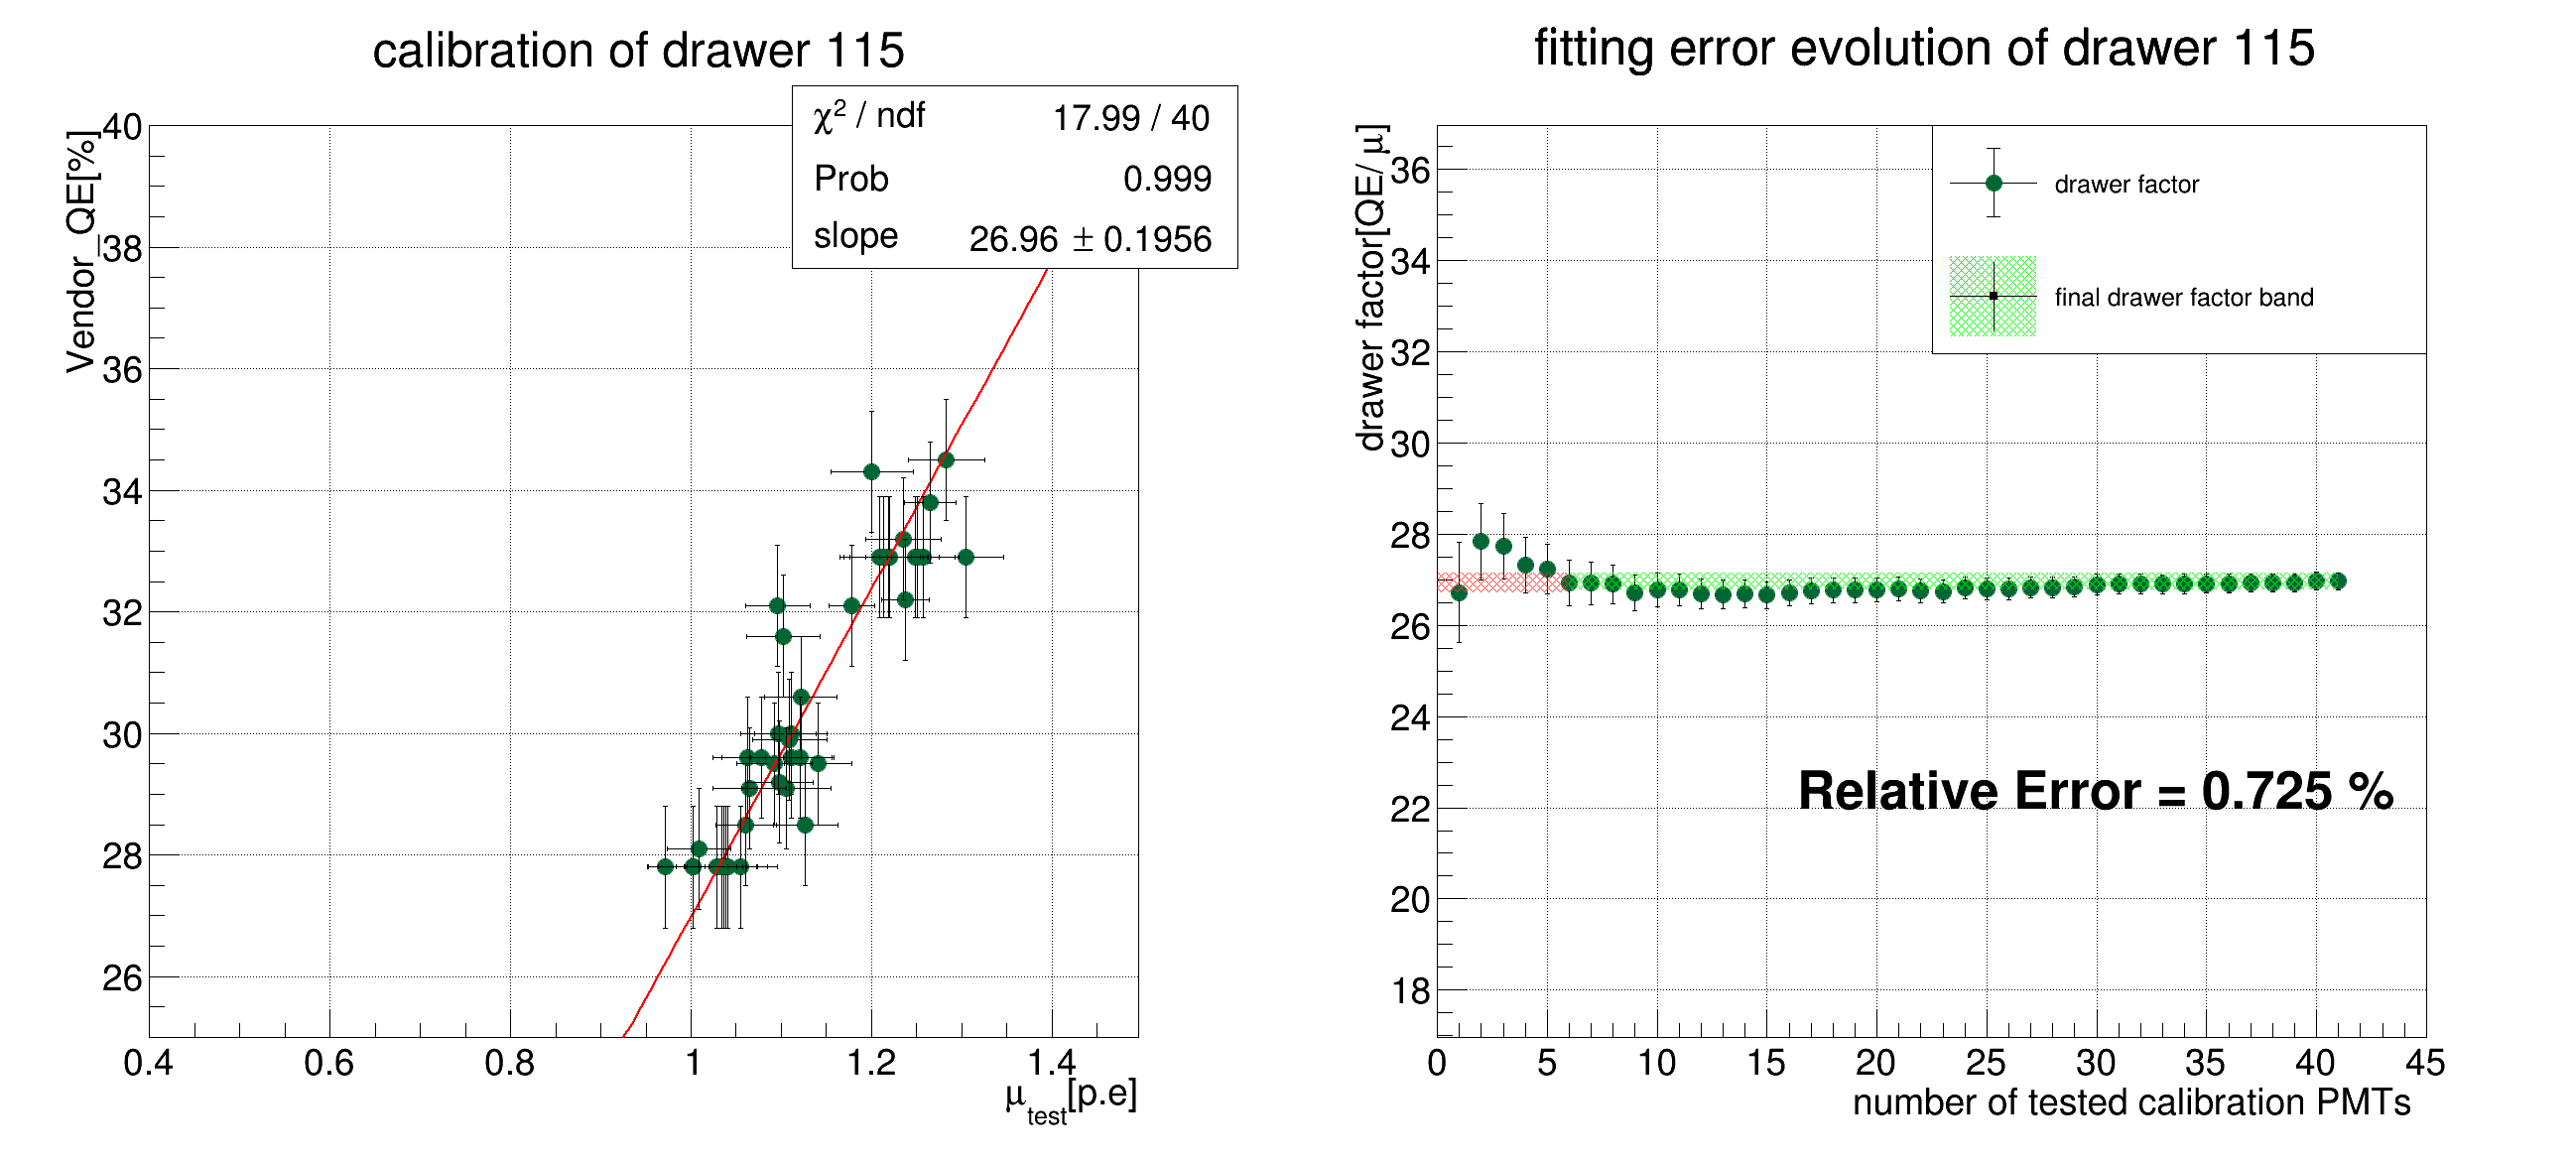
\includegraphics[width=0.45\textwidth]{sta101-14} 
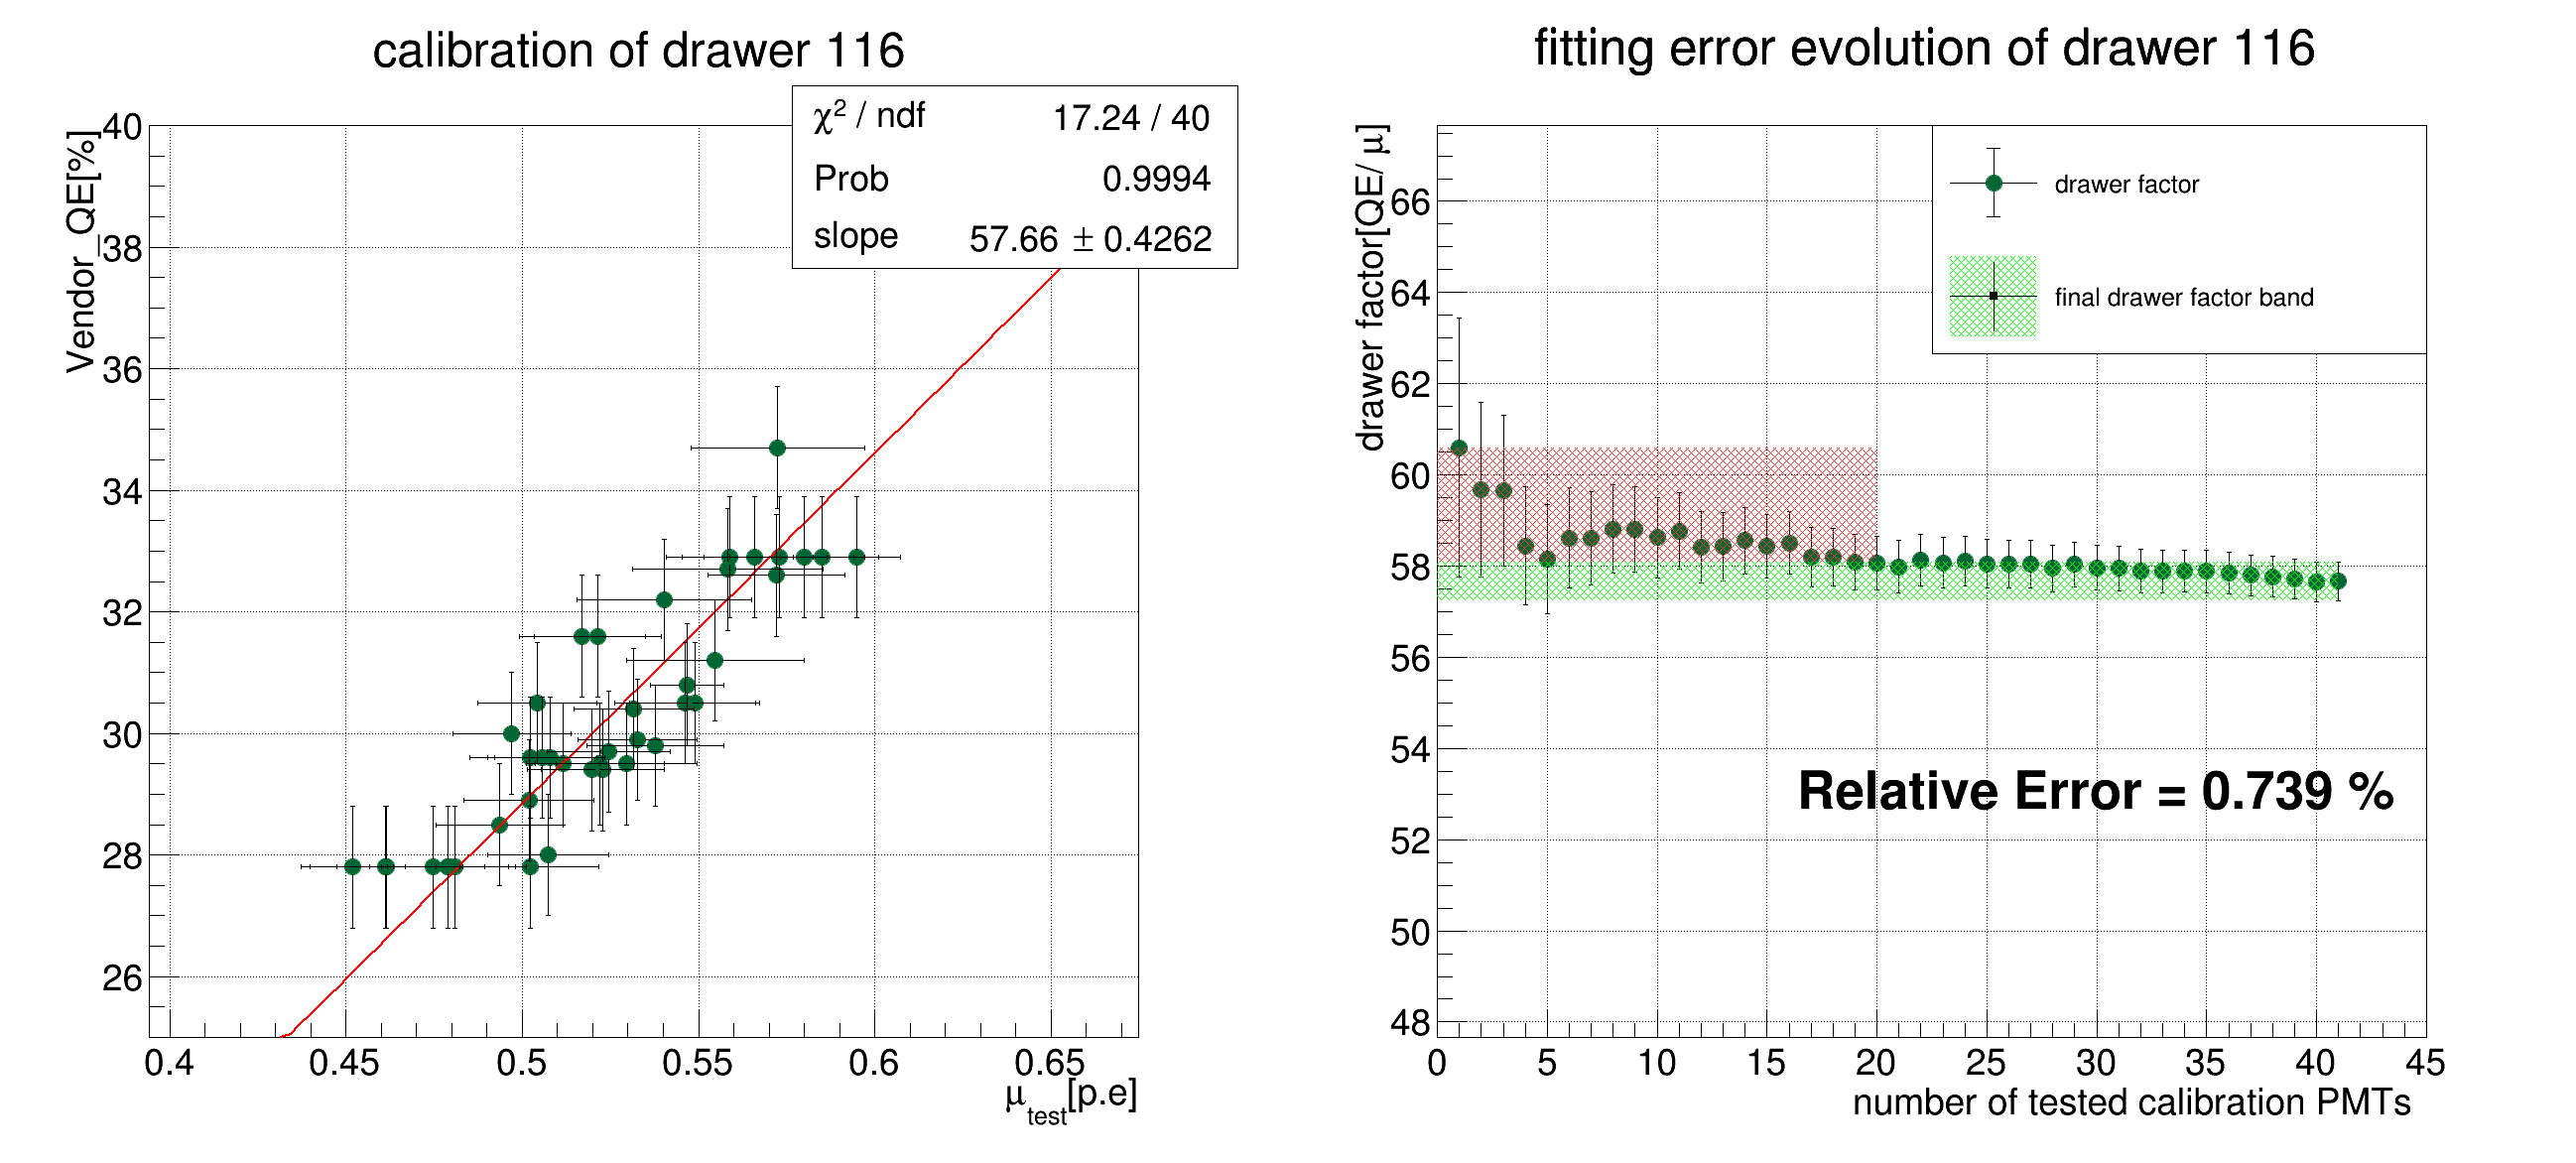
\includegraphics[width=0.45\textwidth]{sta101-15} 
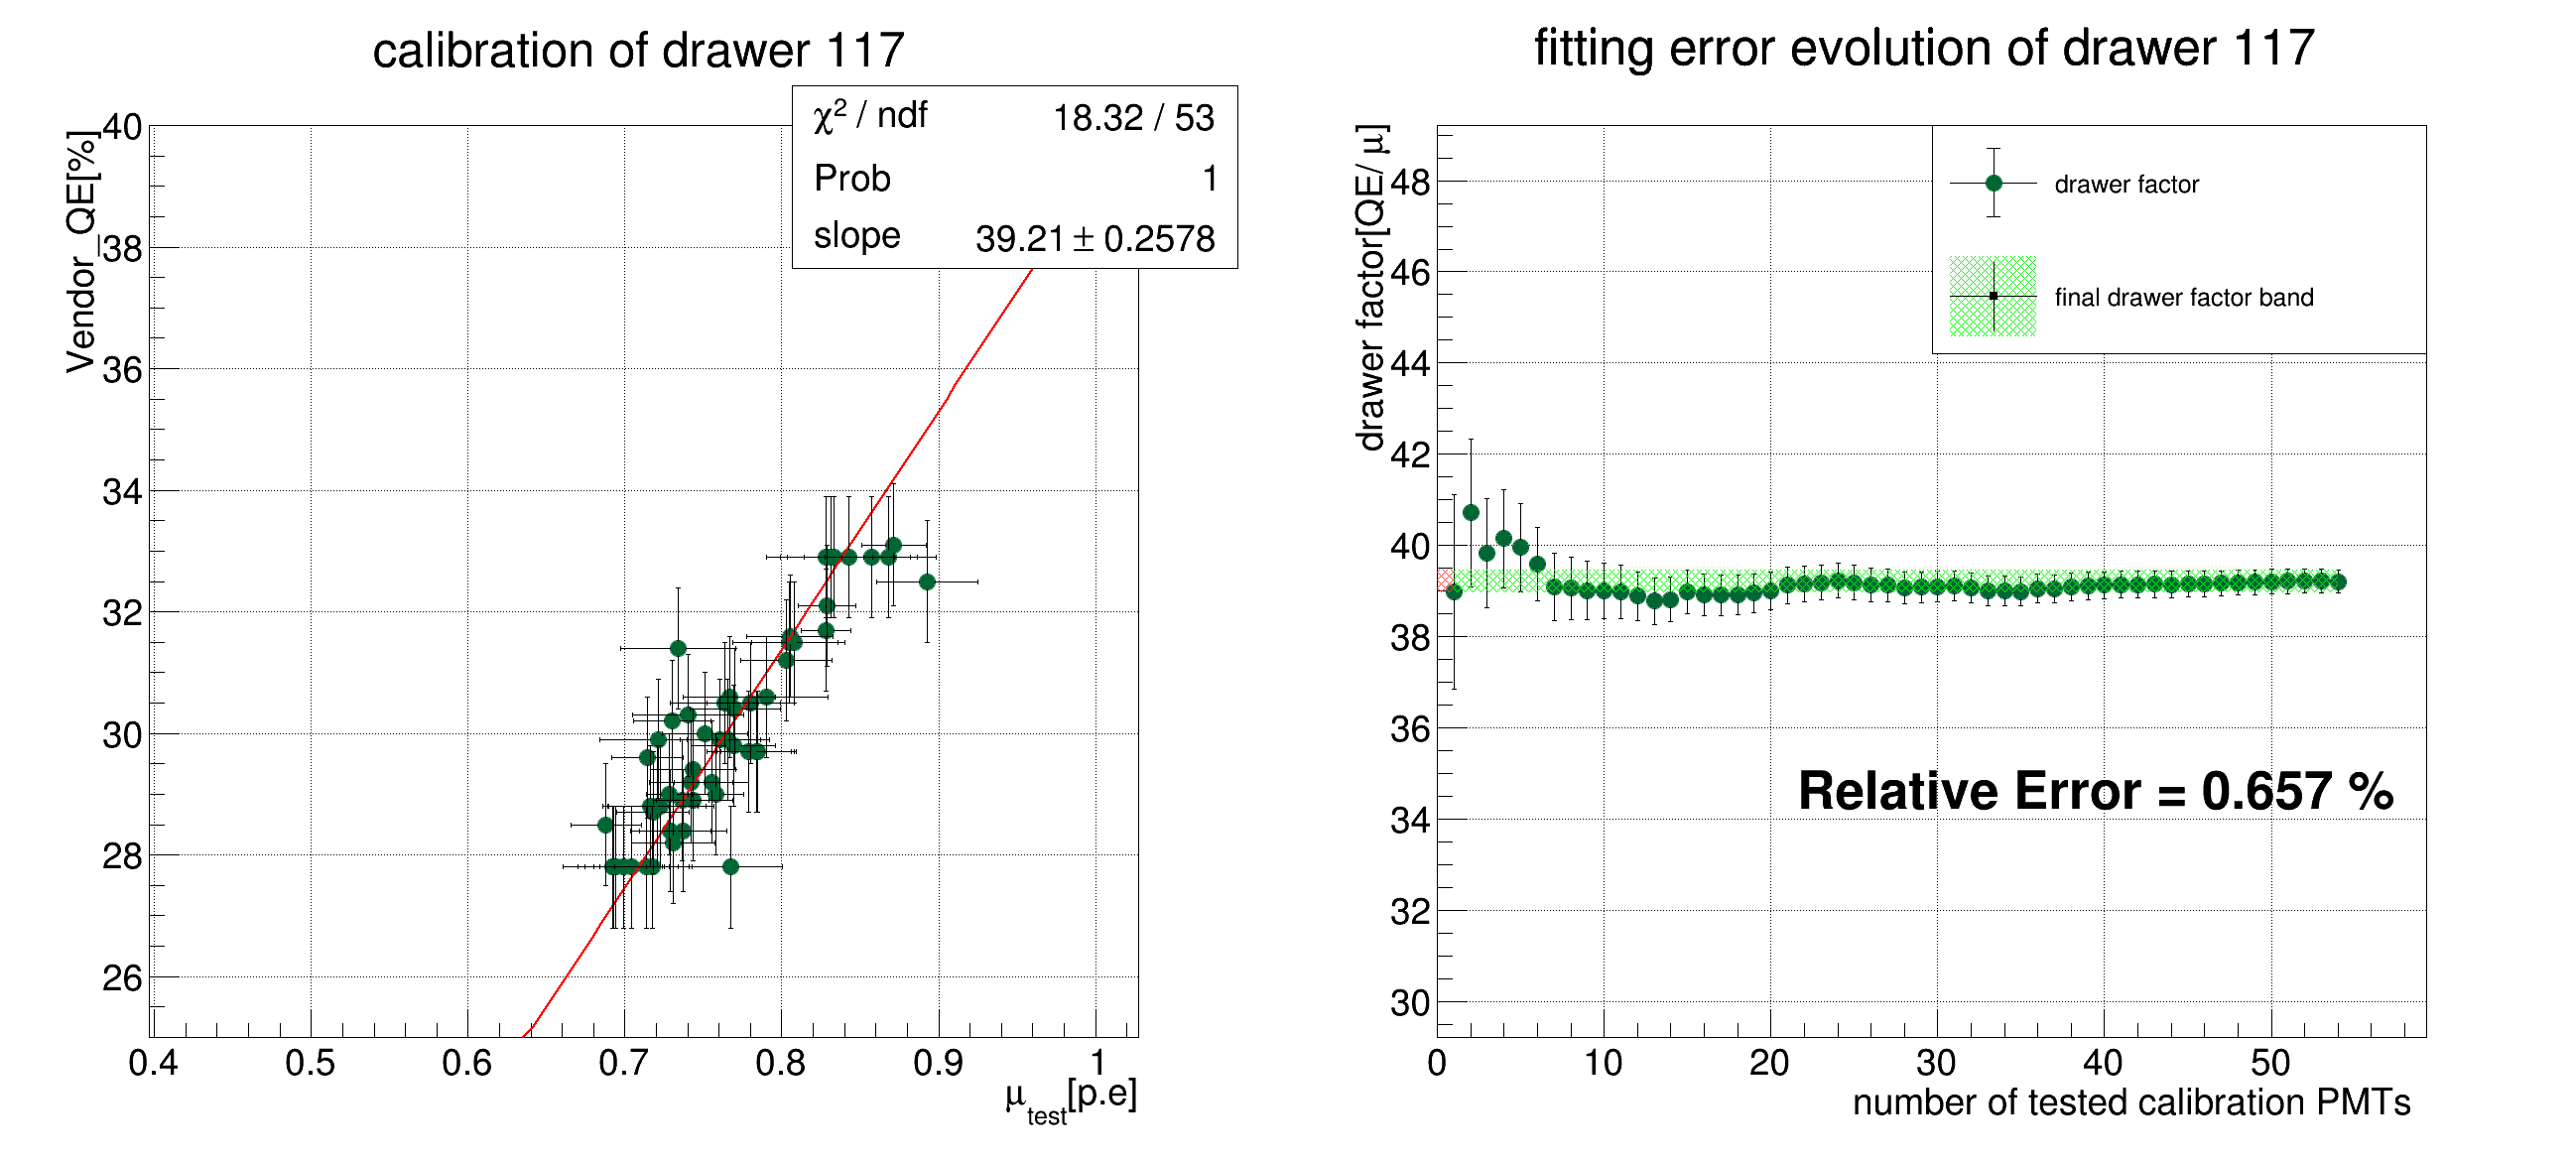
\includegraphics[width=0.45\textwidth]{sta101-16} 
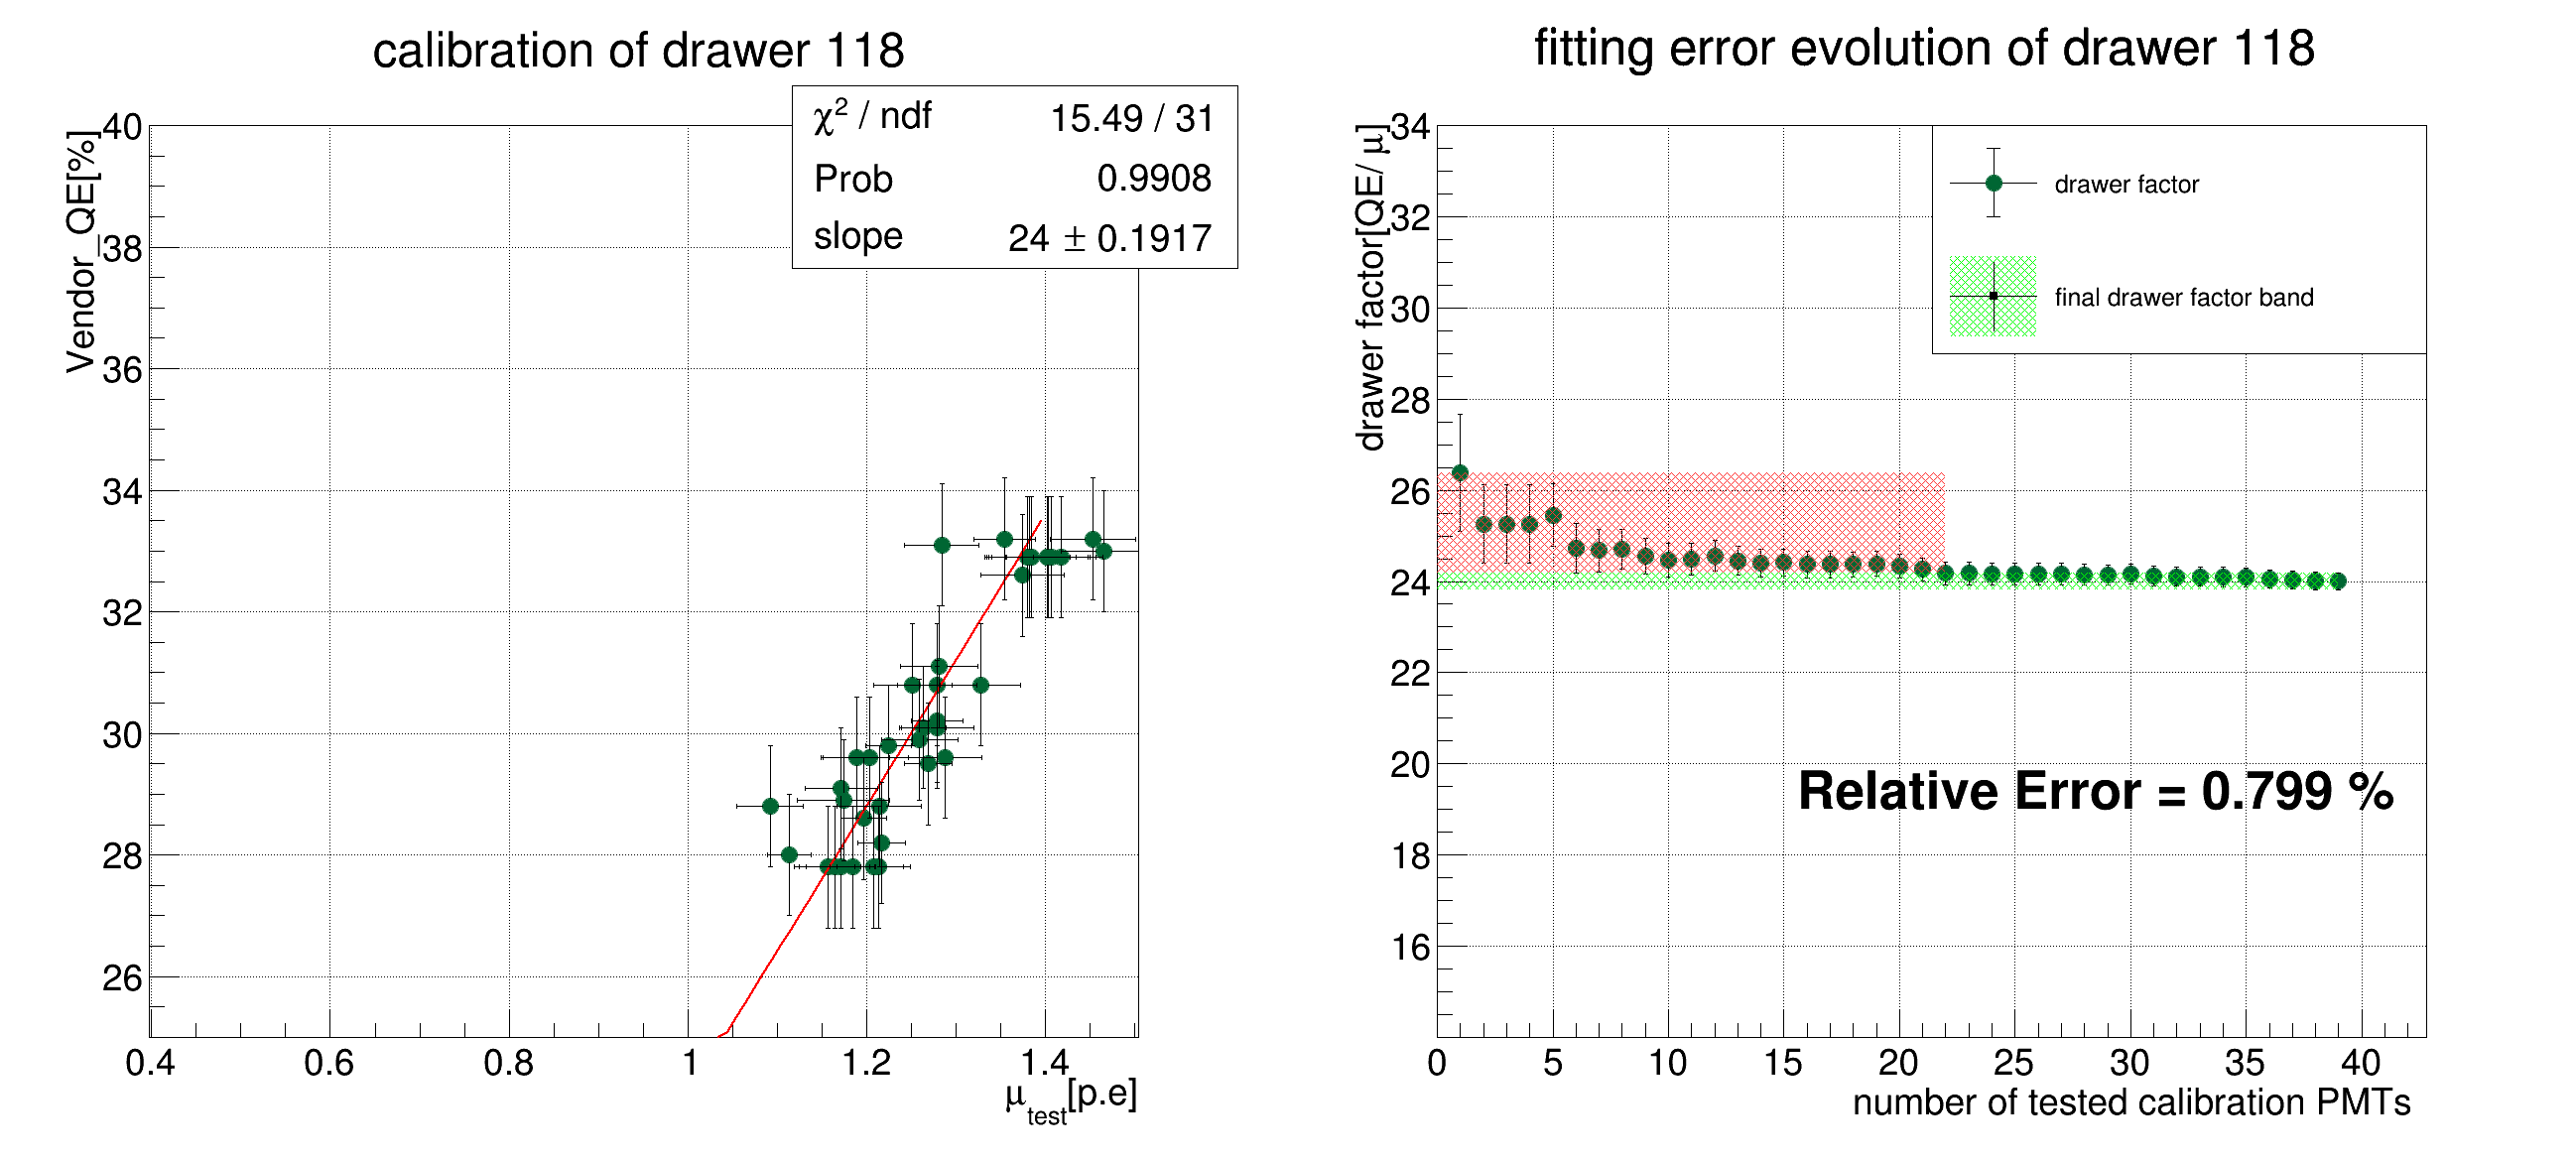
\includegraphics[width=0.45\textwidth]{sta101-17} 
\end{frame}
\begin{frame}{drawer-calibration}
\vspace{-.5cm}
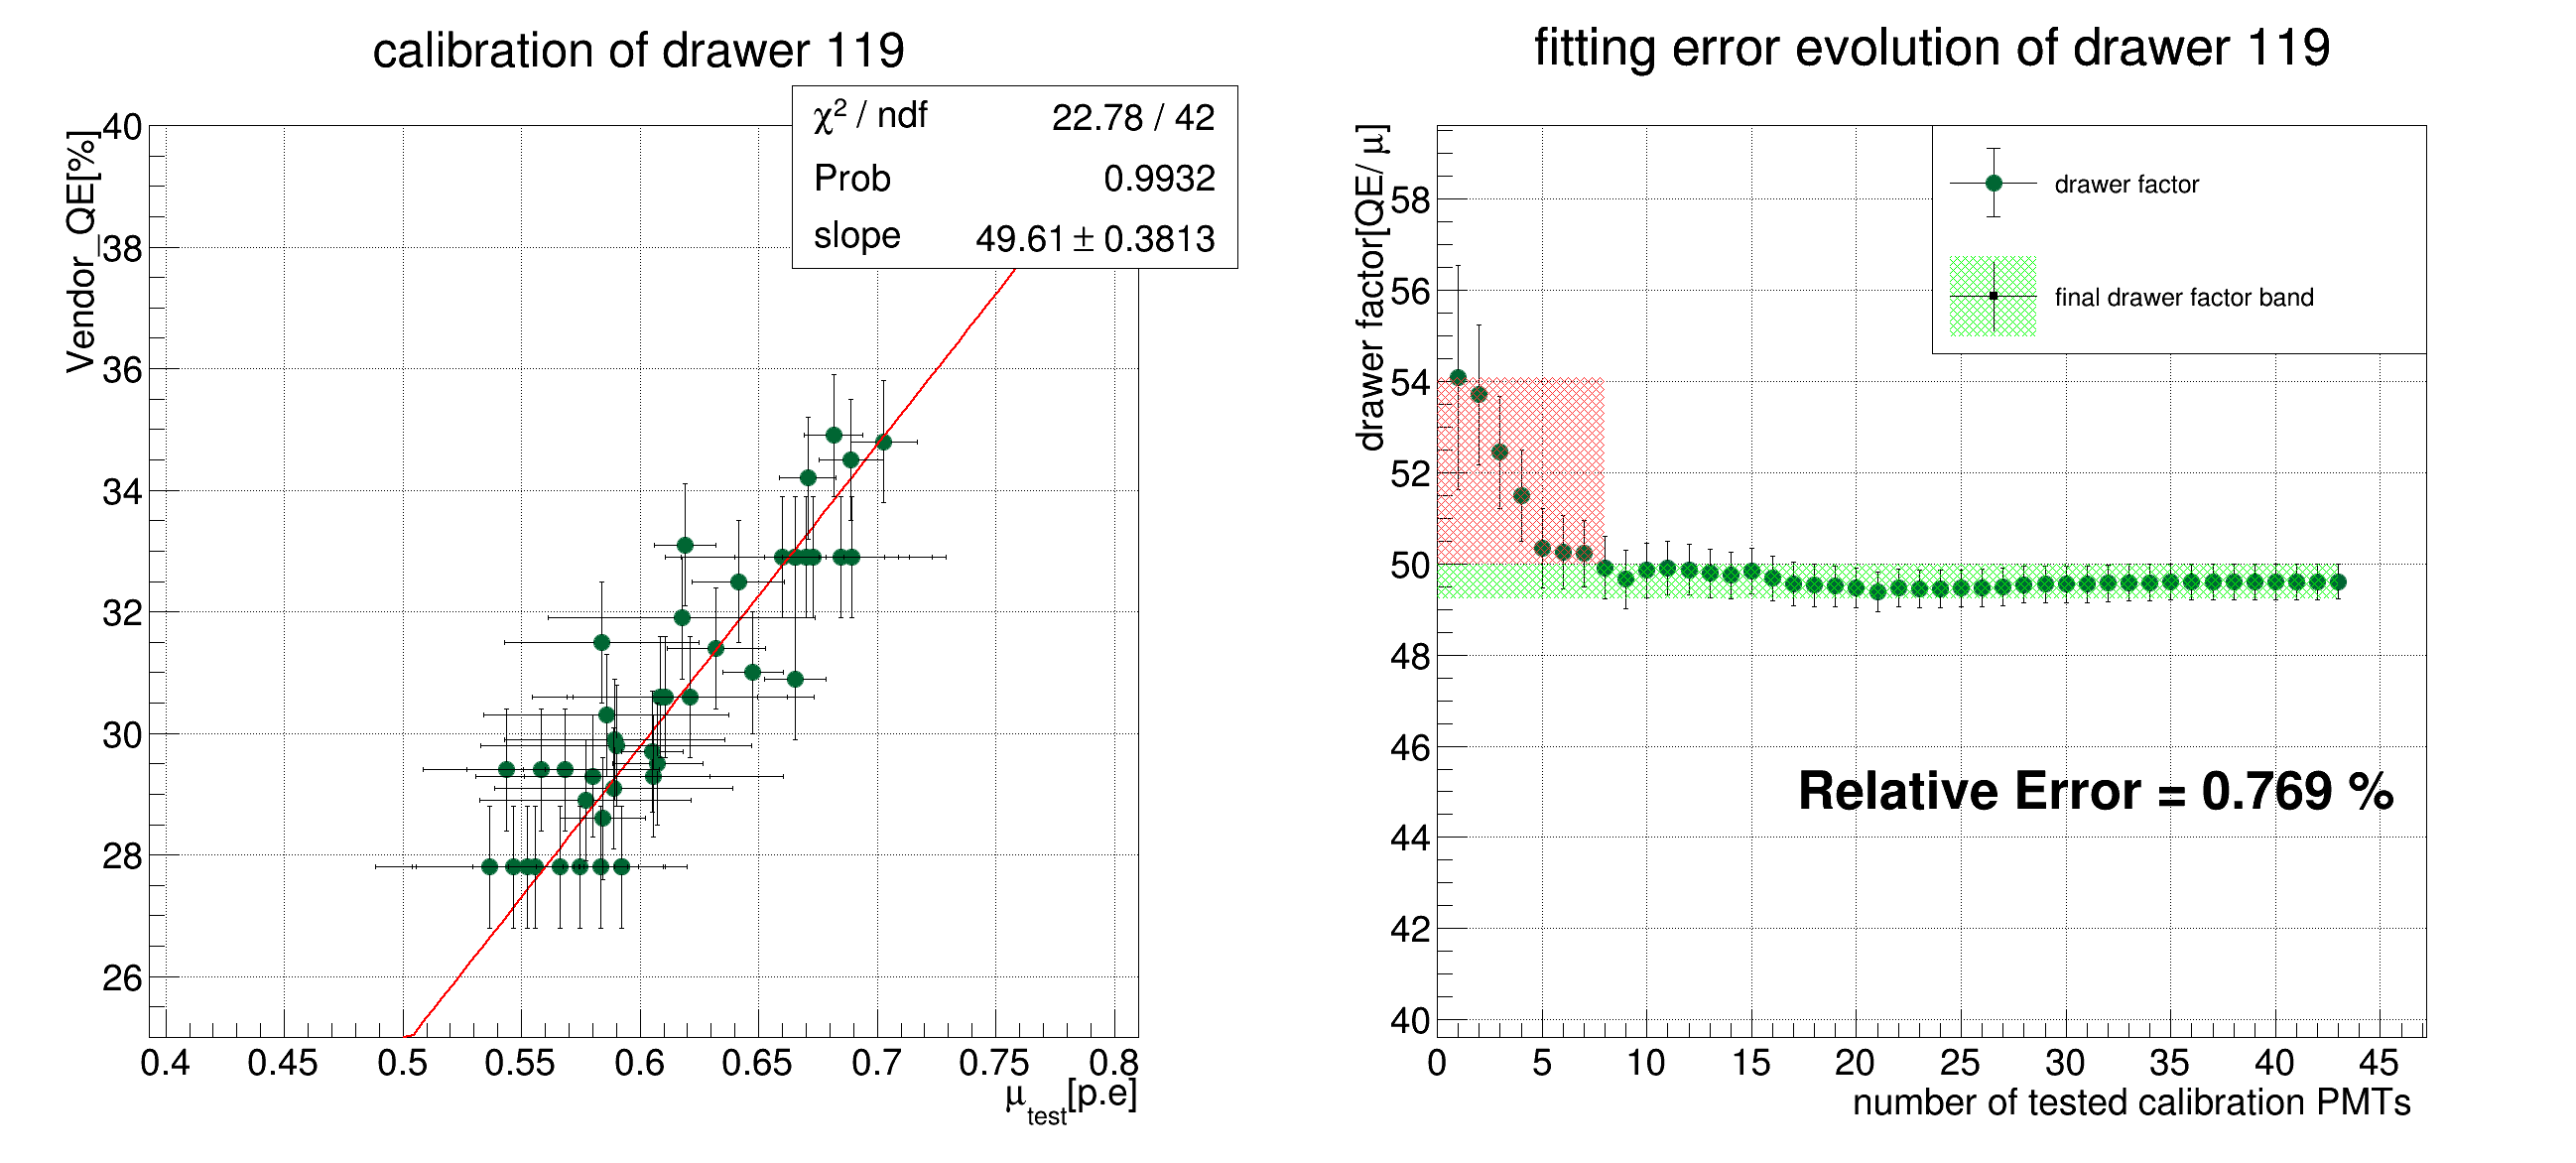
\includegraphics[width=0.45\textwidth]{sta101-18} 
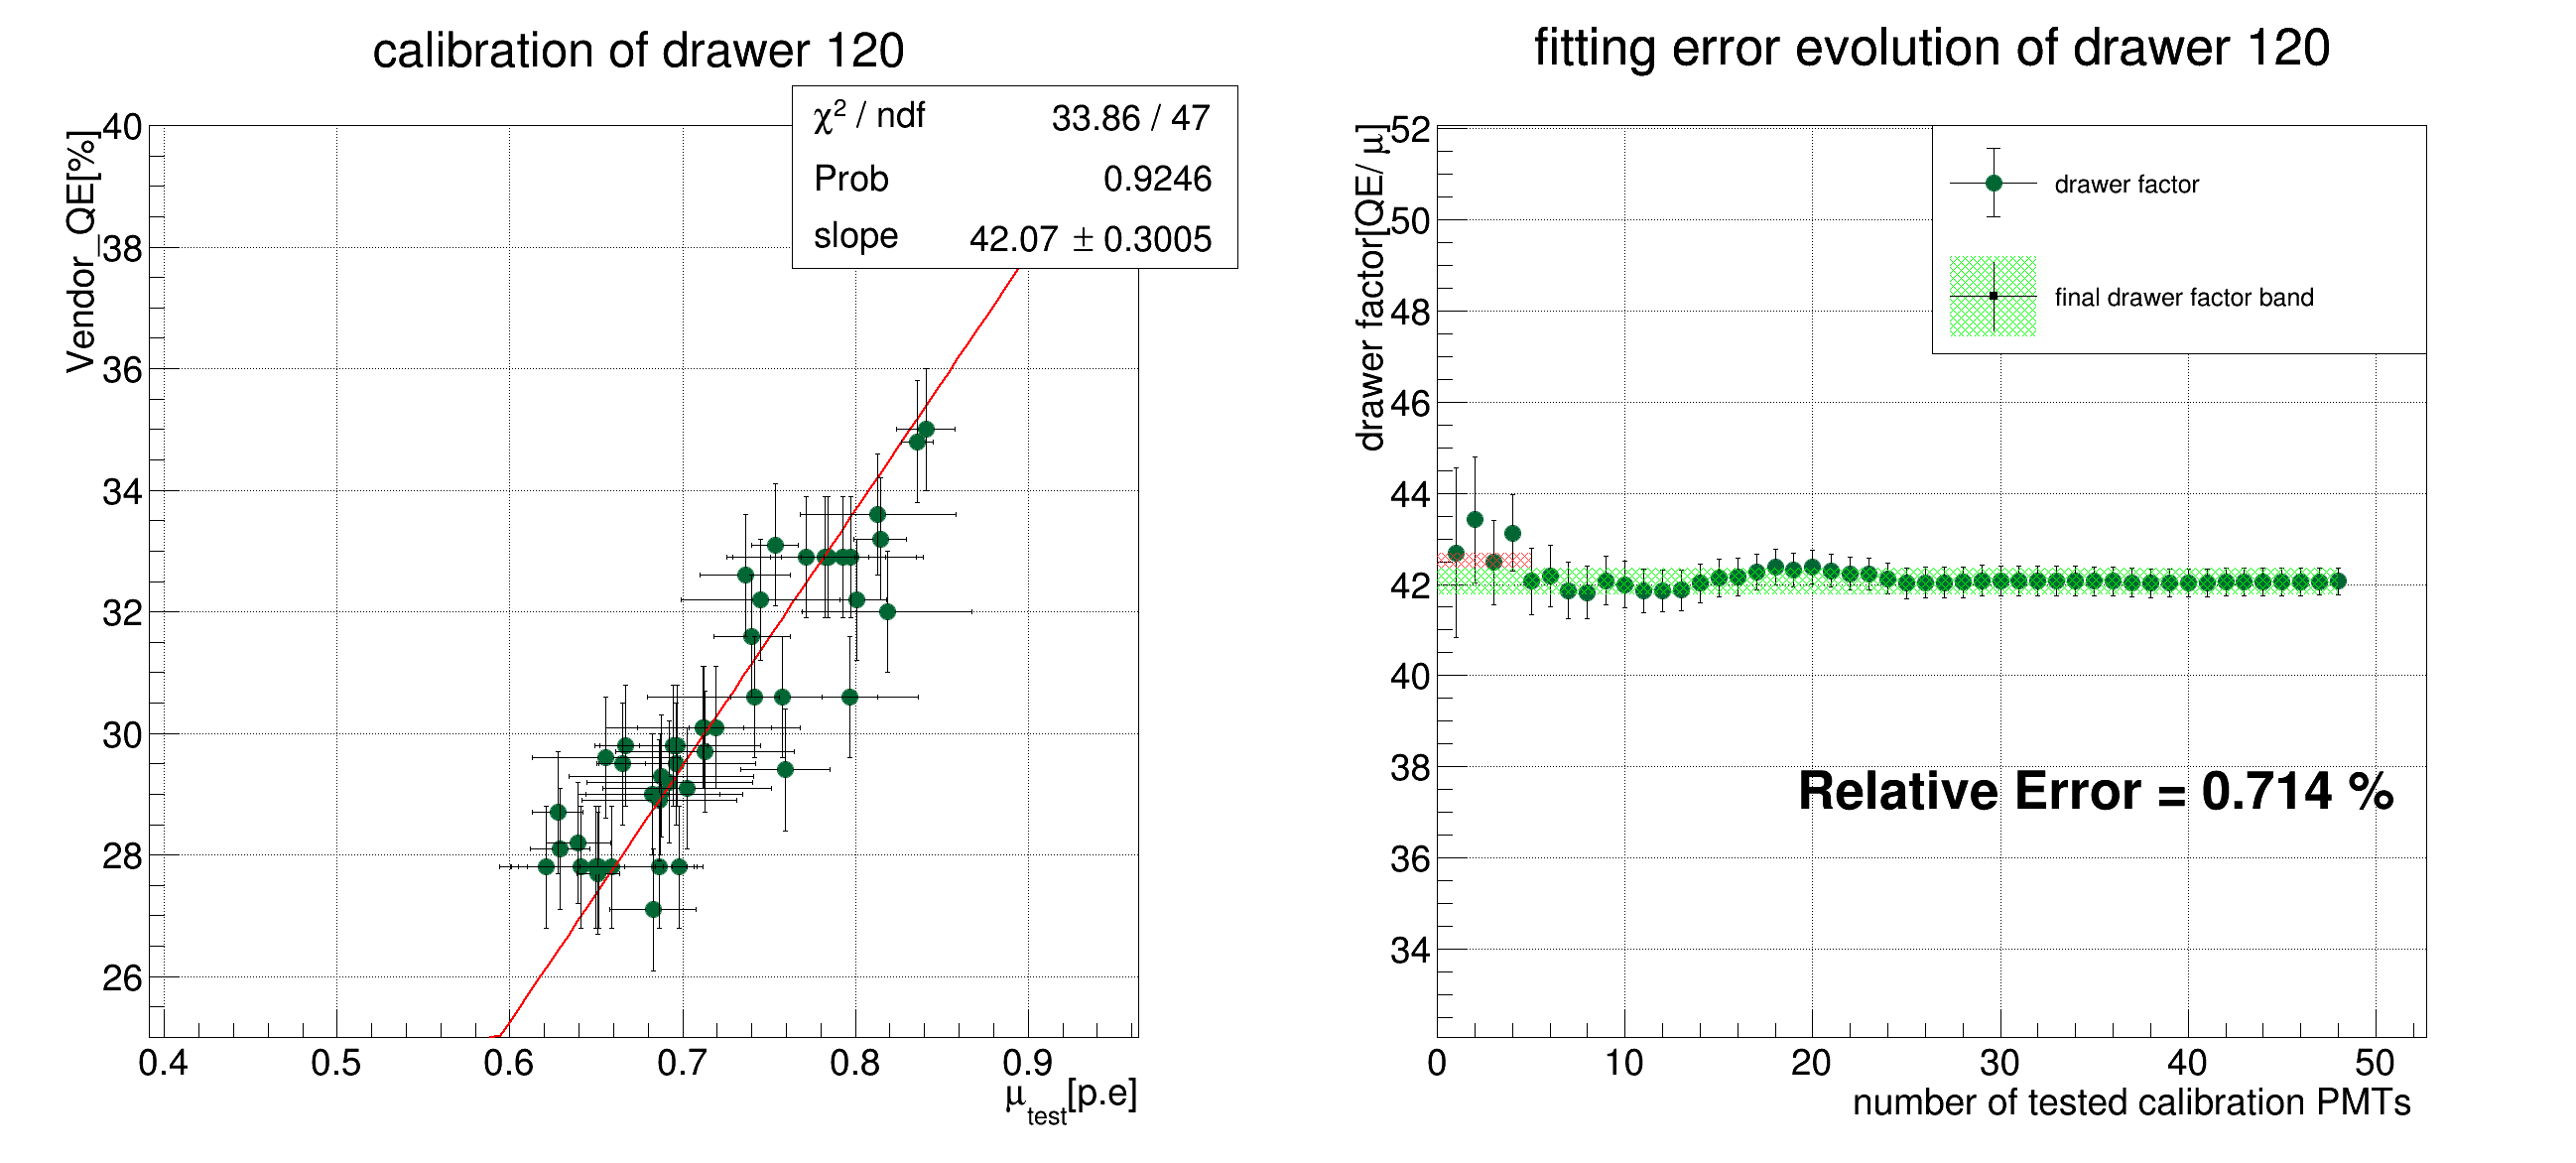
\includegraphics[width=0.45\textwidth]{sta101-19} 
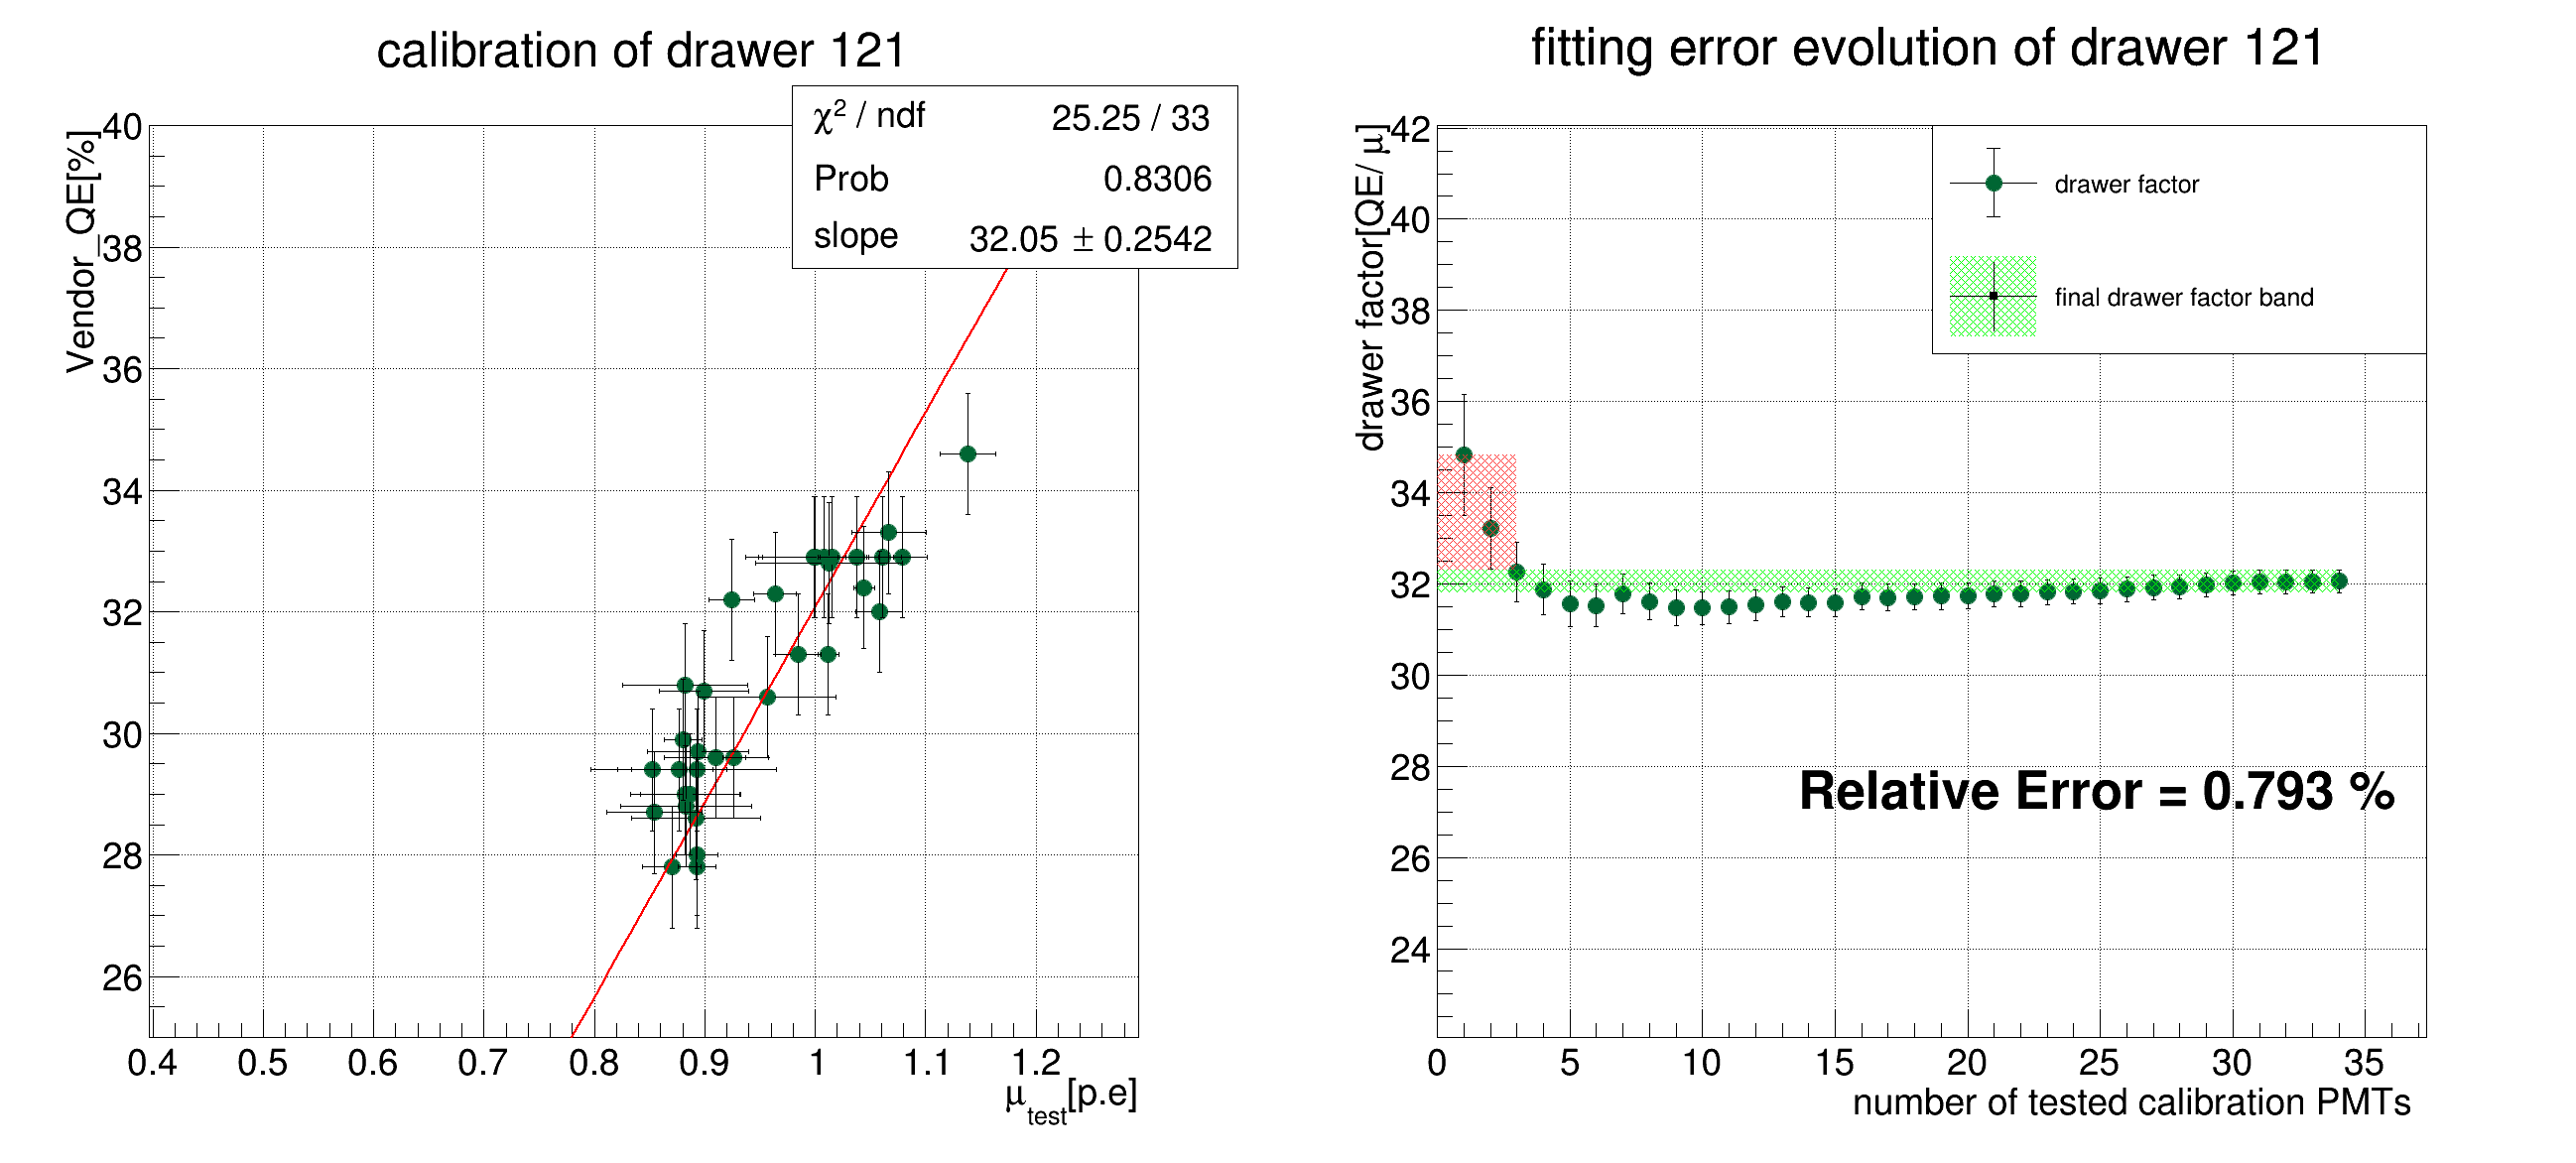
\includegraphics[width=0.45\textwidth]{sta101-20} 
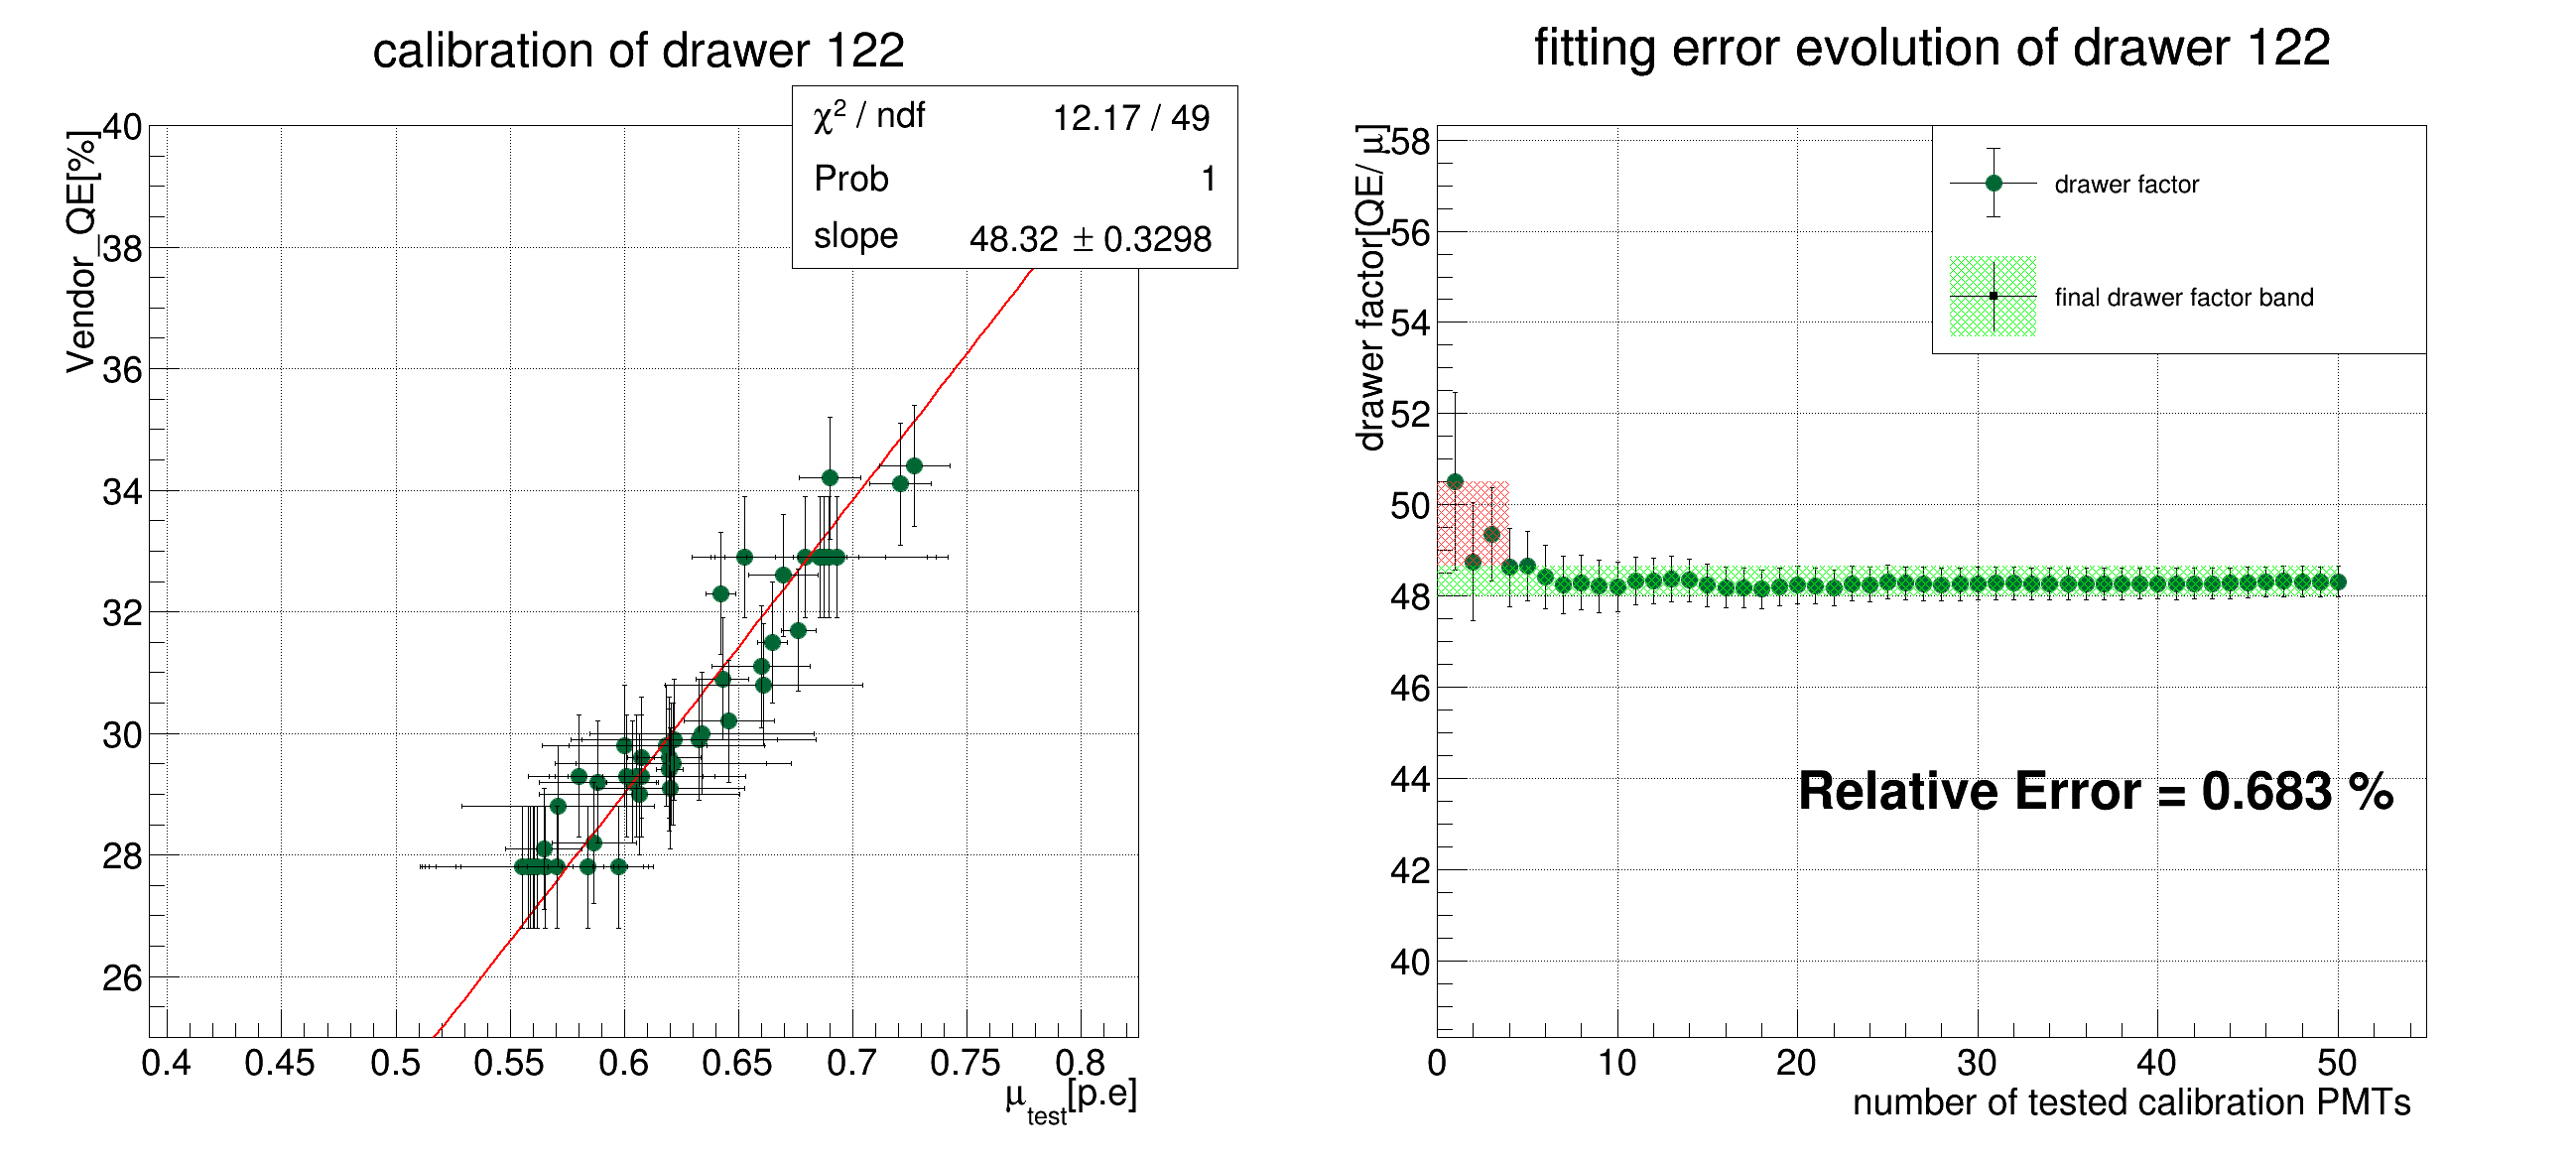
\includegraphics[width=0.45\textwidth]{sta101-21} 
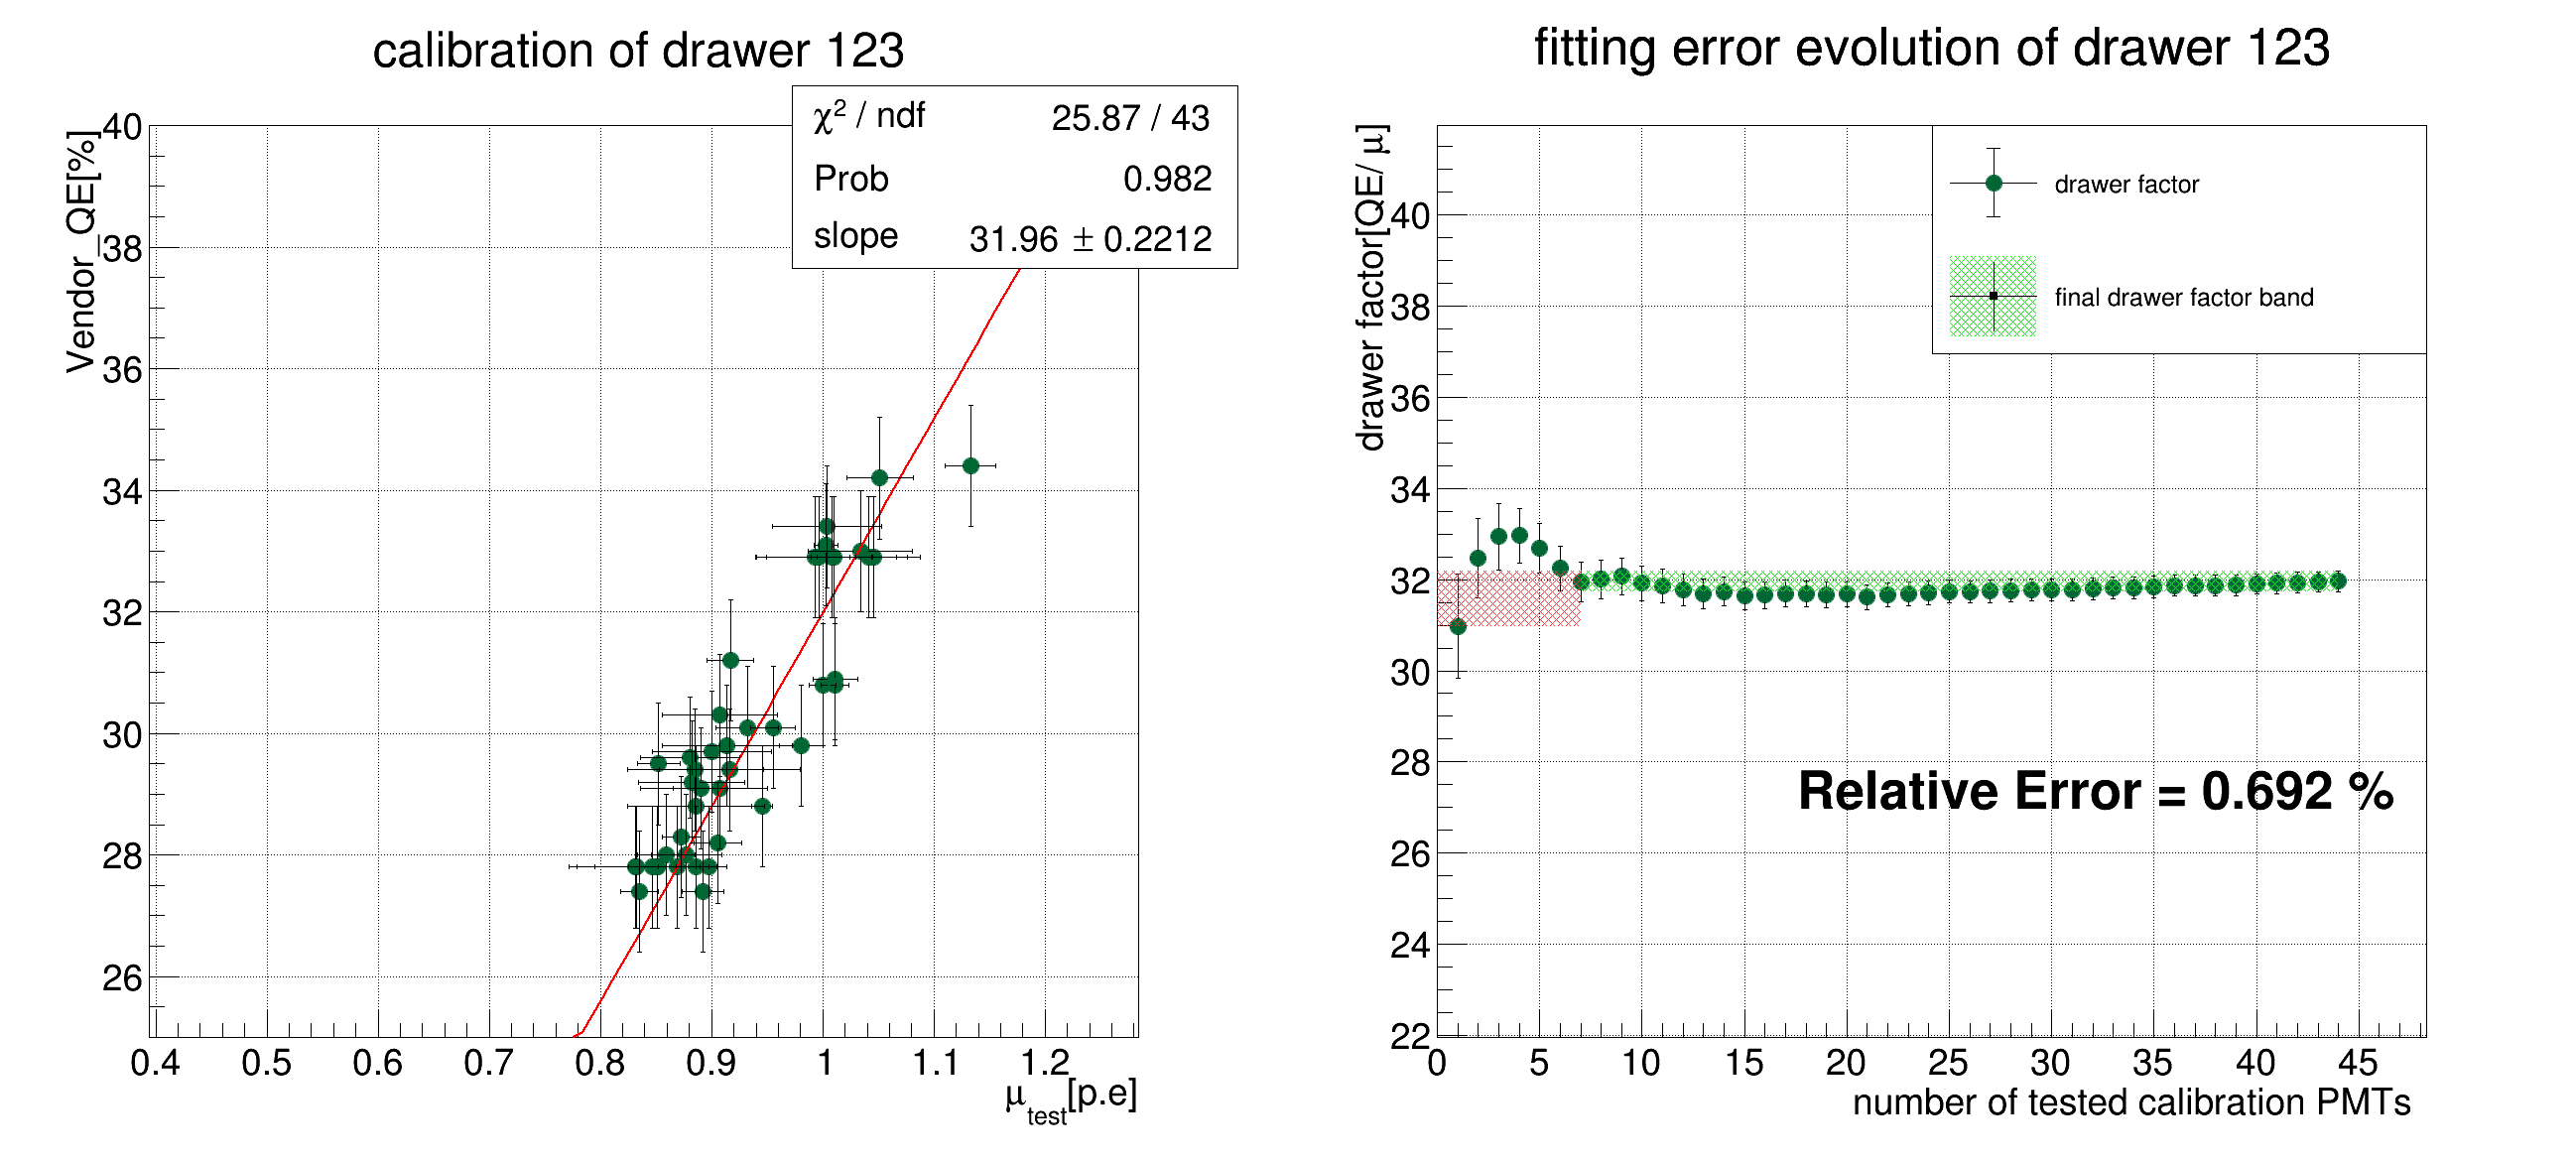
\includegraphics[width=0.45\textwidth]{sta101-22} 
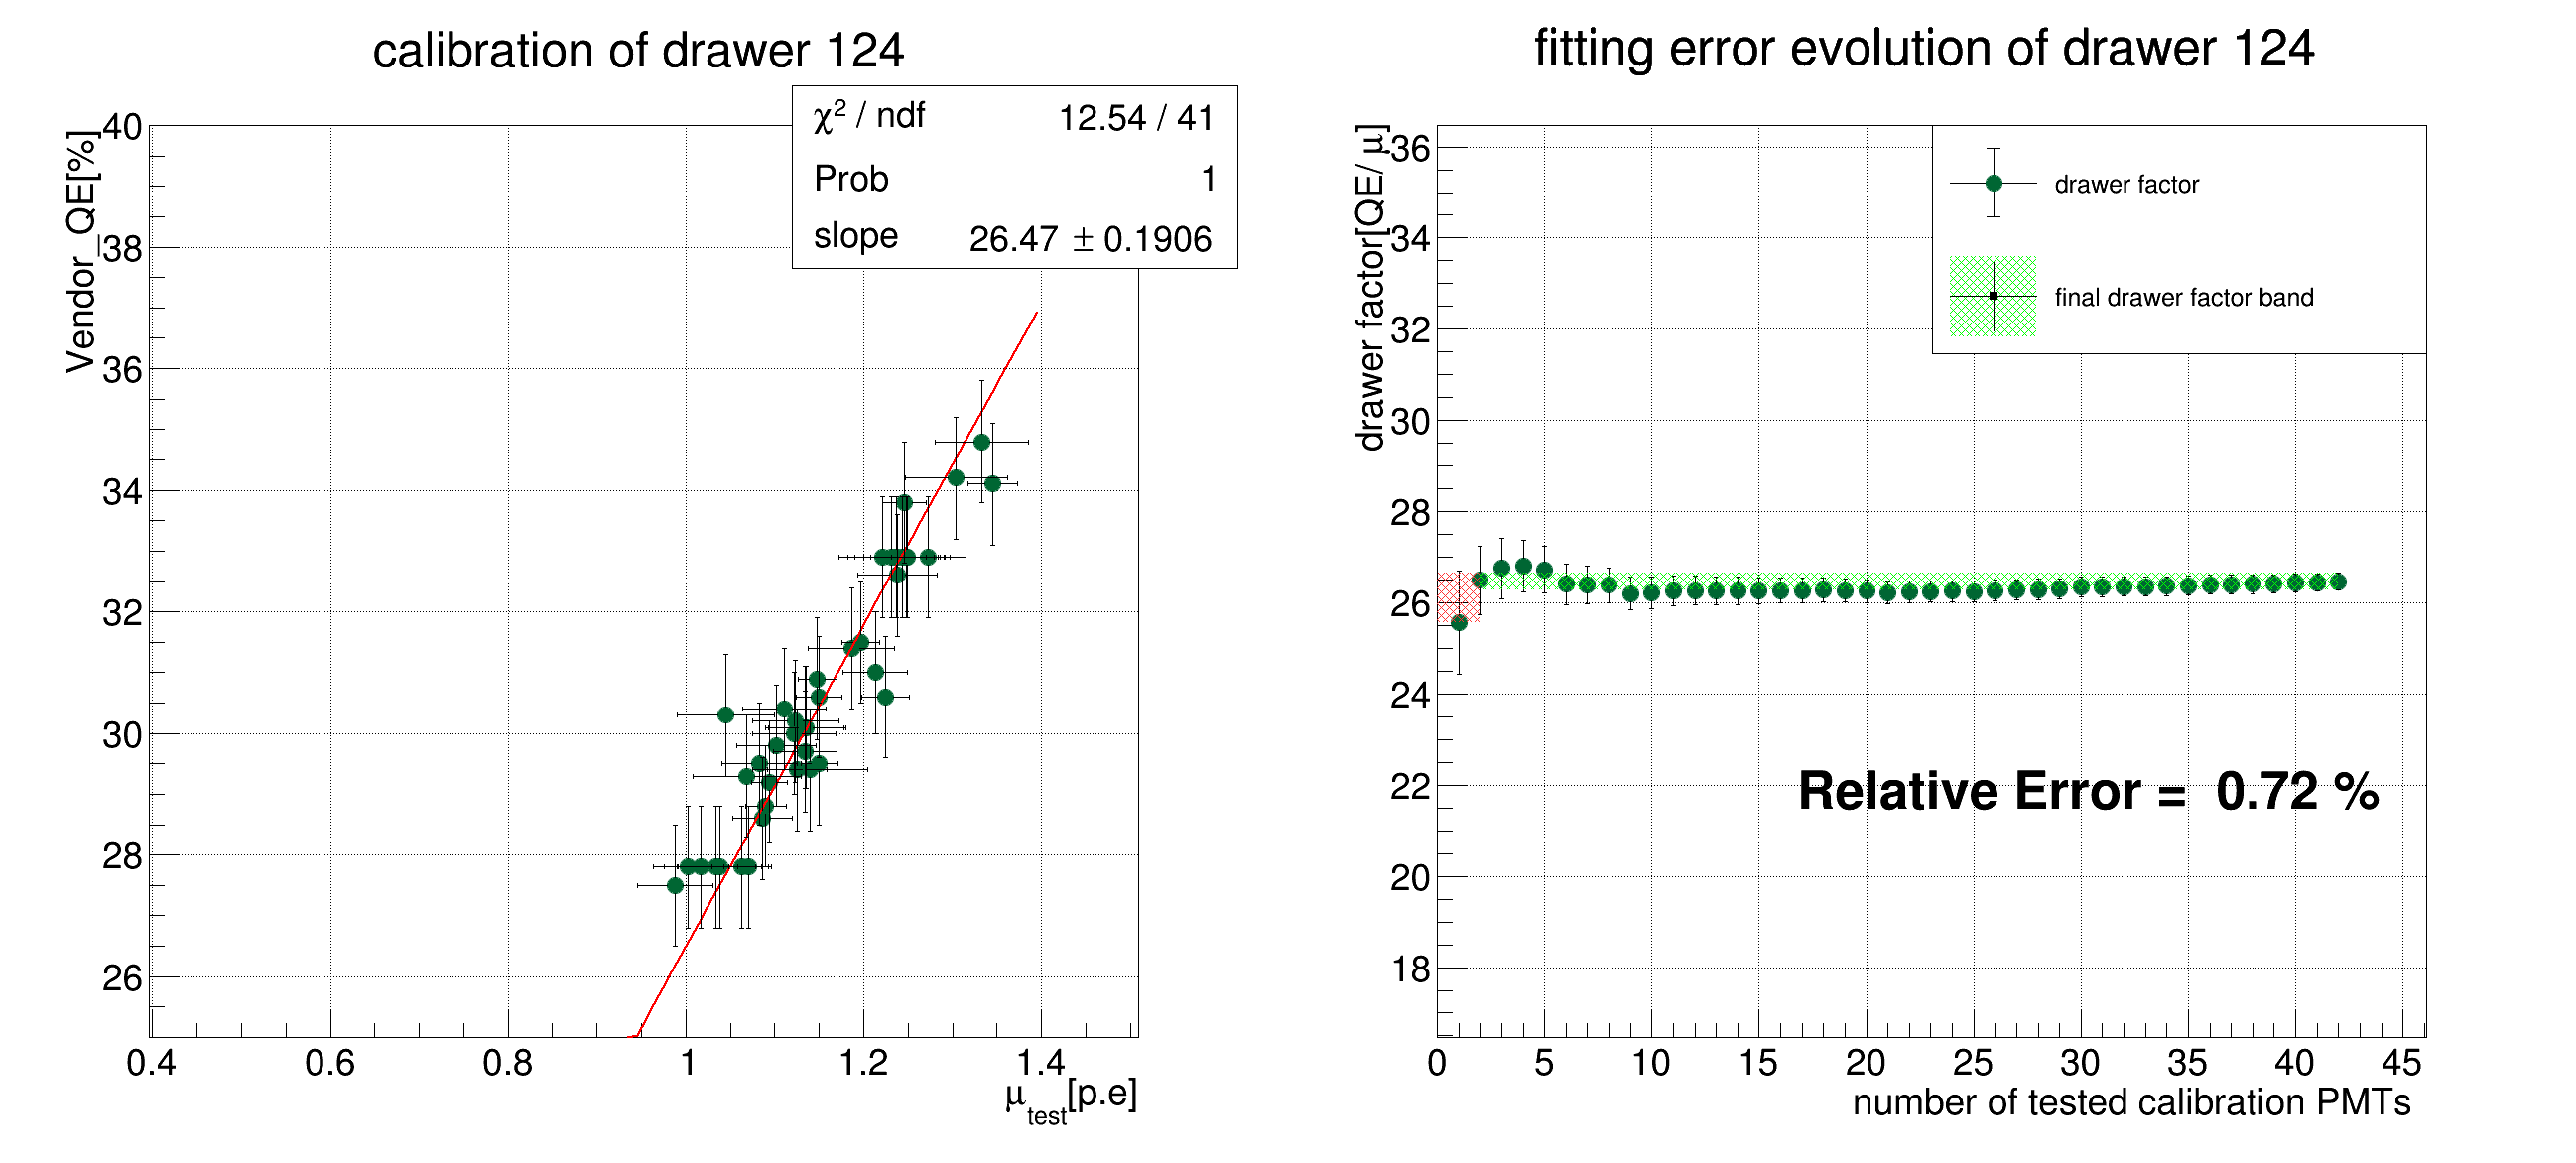
\includegraphics[width=0.45\textwidth]{sta101-23} 
\end{frame}
\begin{frame}{drawer-calibration}
\vspace{-.5cm}
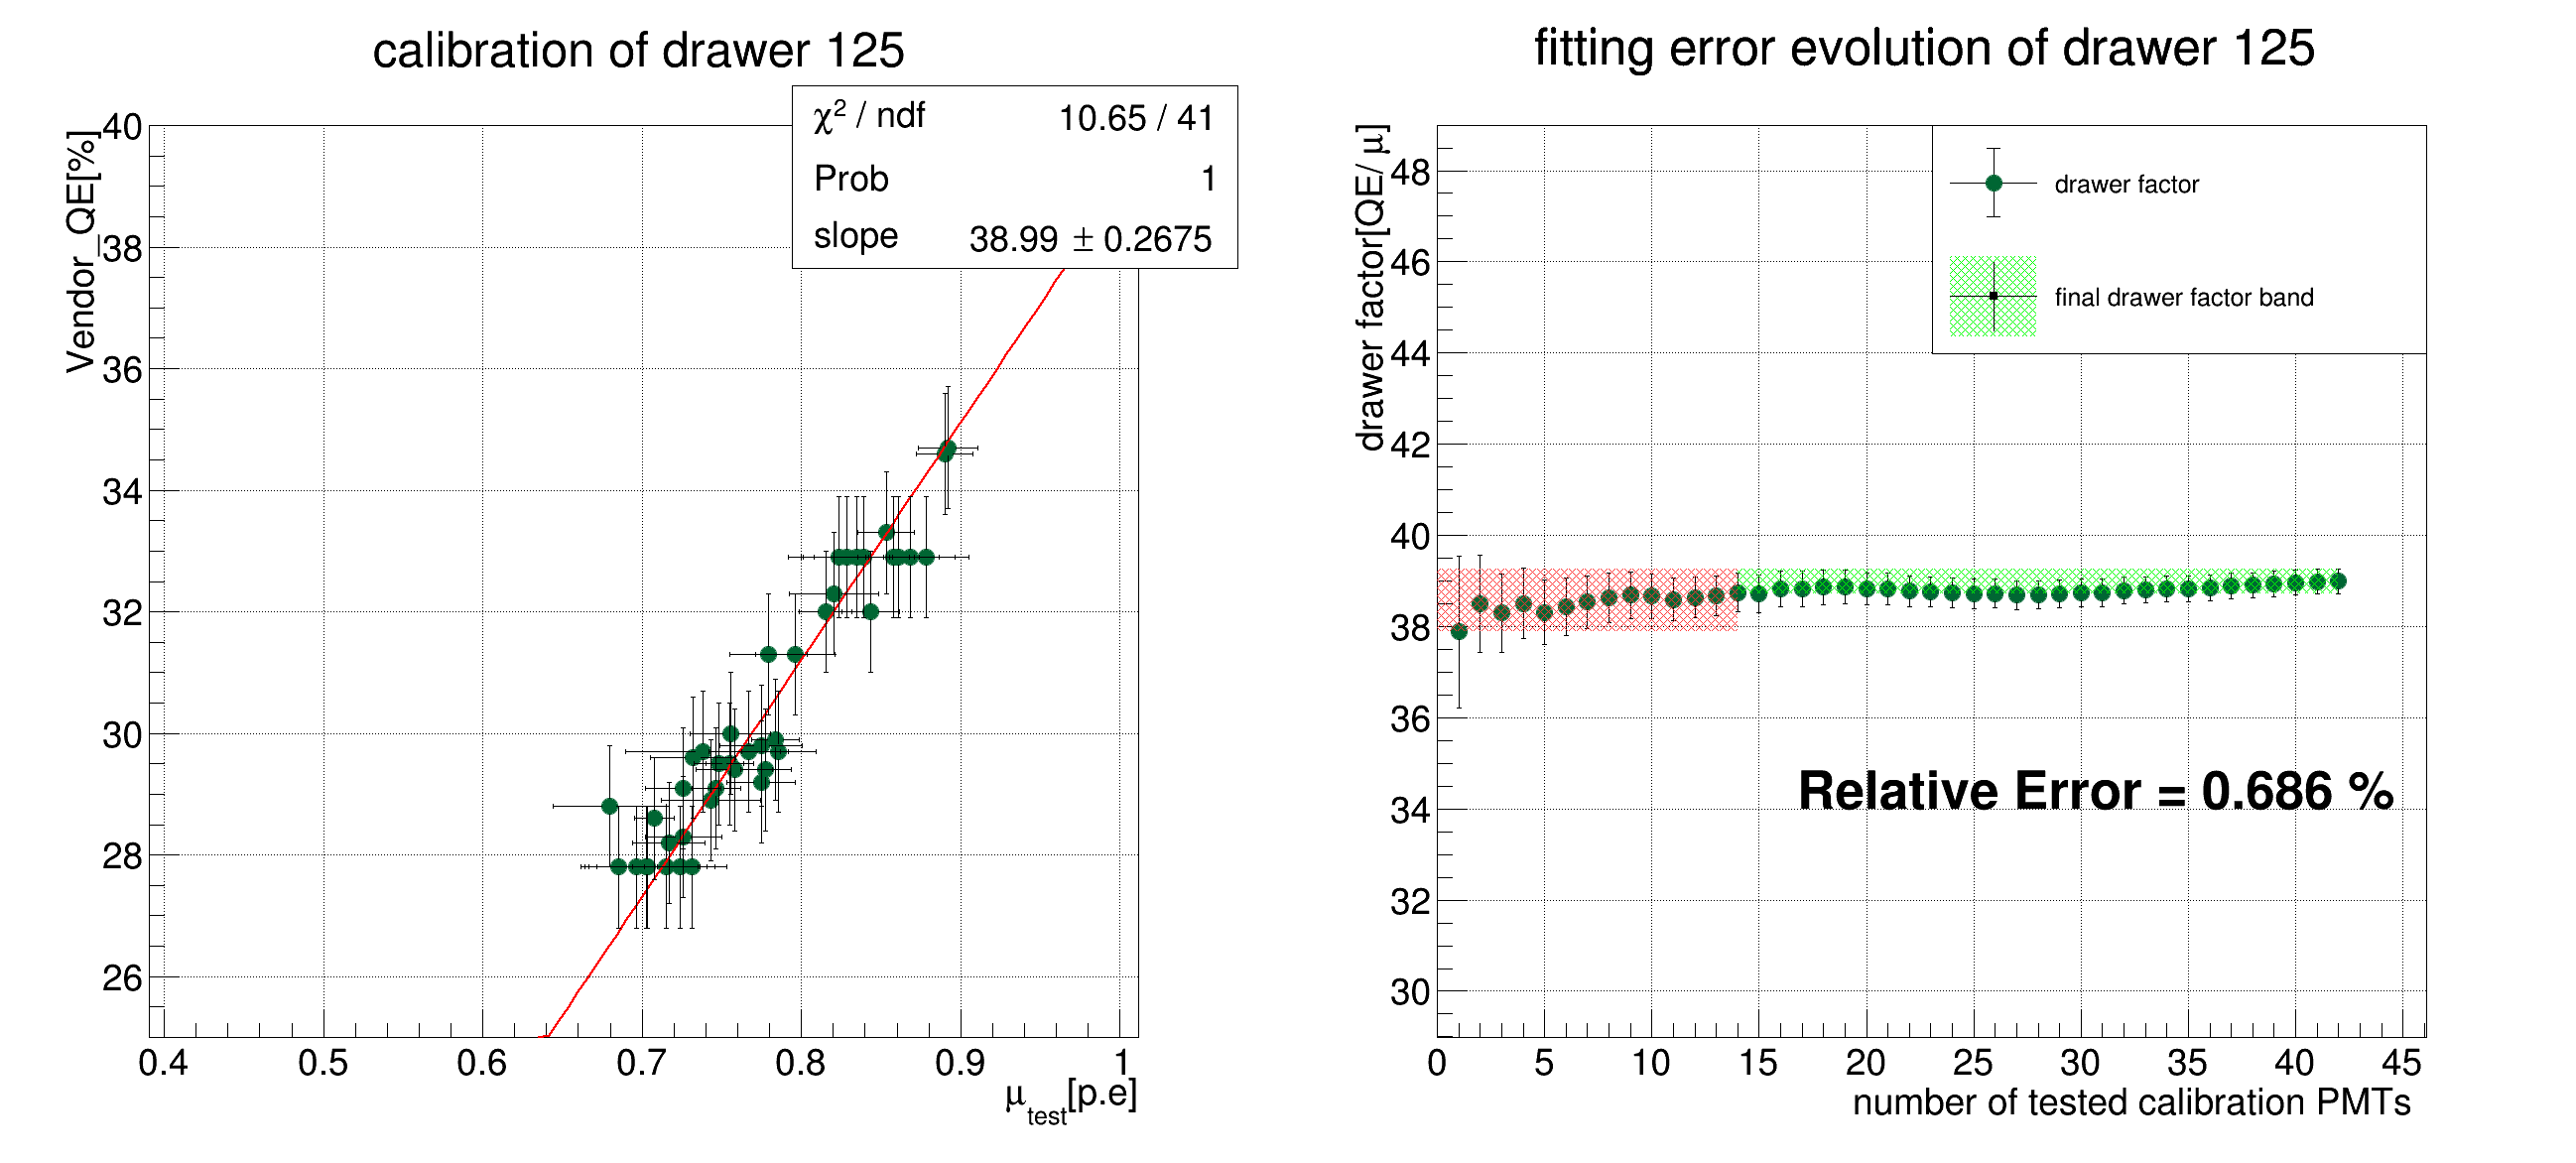
\includegraphics[width=0.45\textwidth]{sta101-24} 
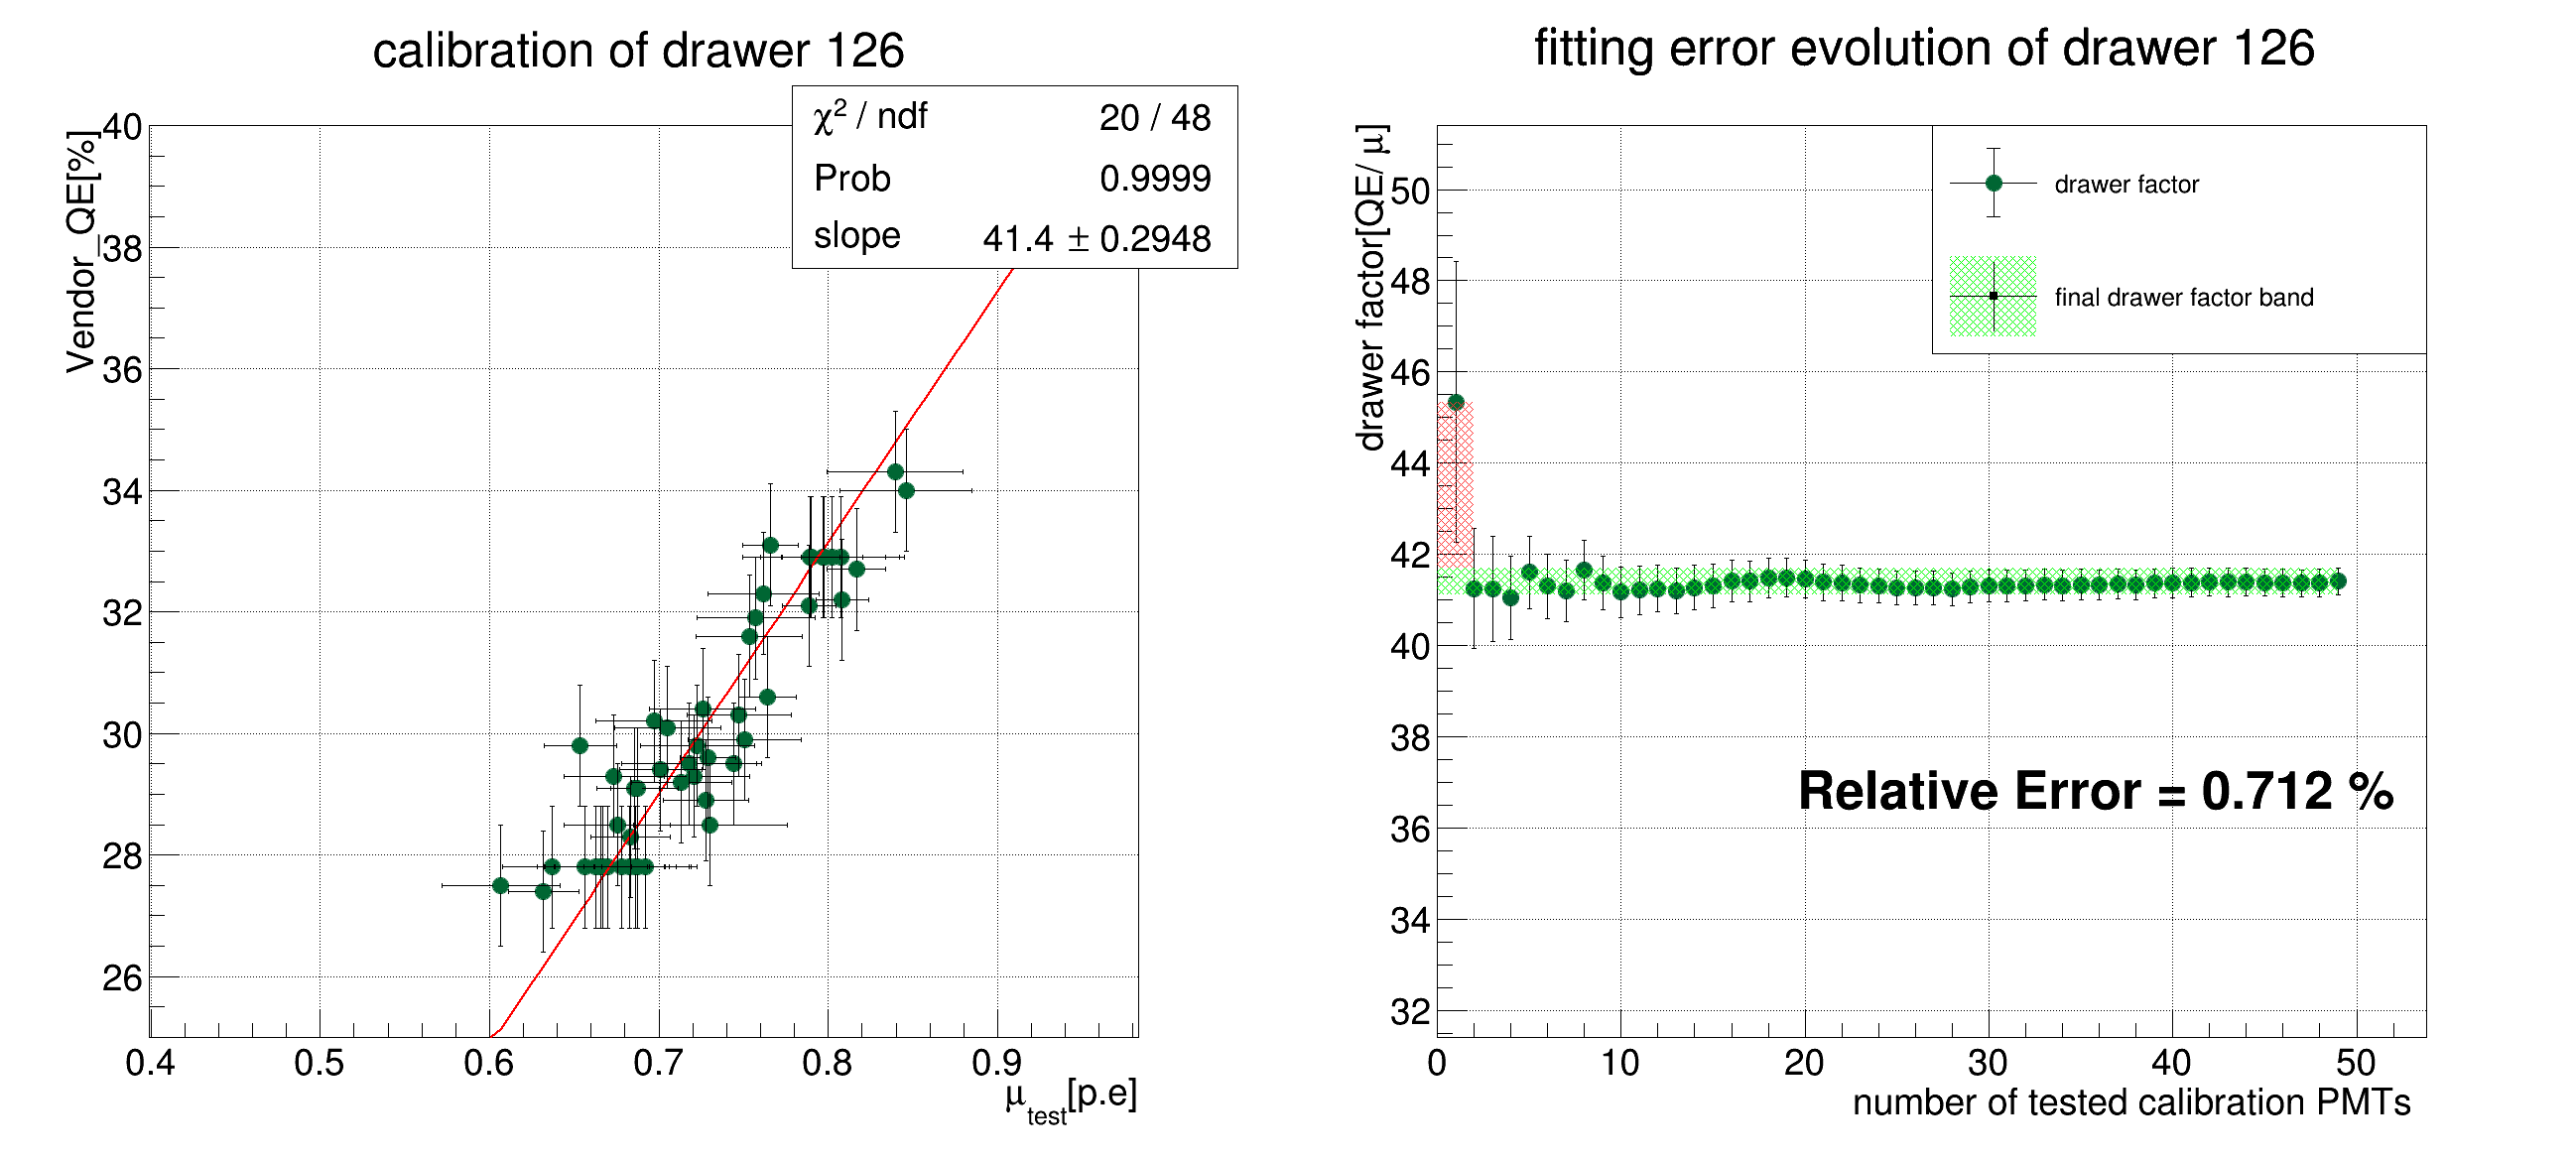
\includegraphics[width=0.45\textwidth]{sta101-25} 
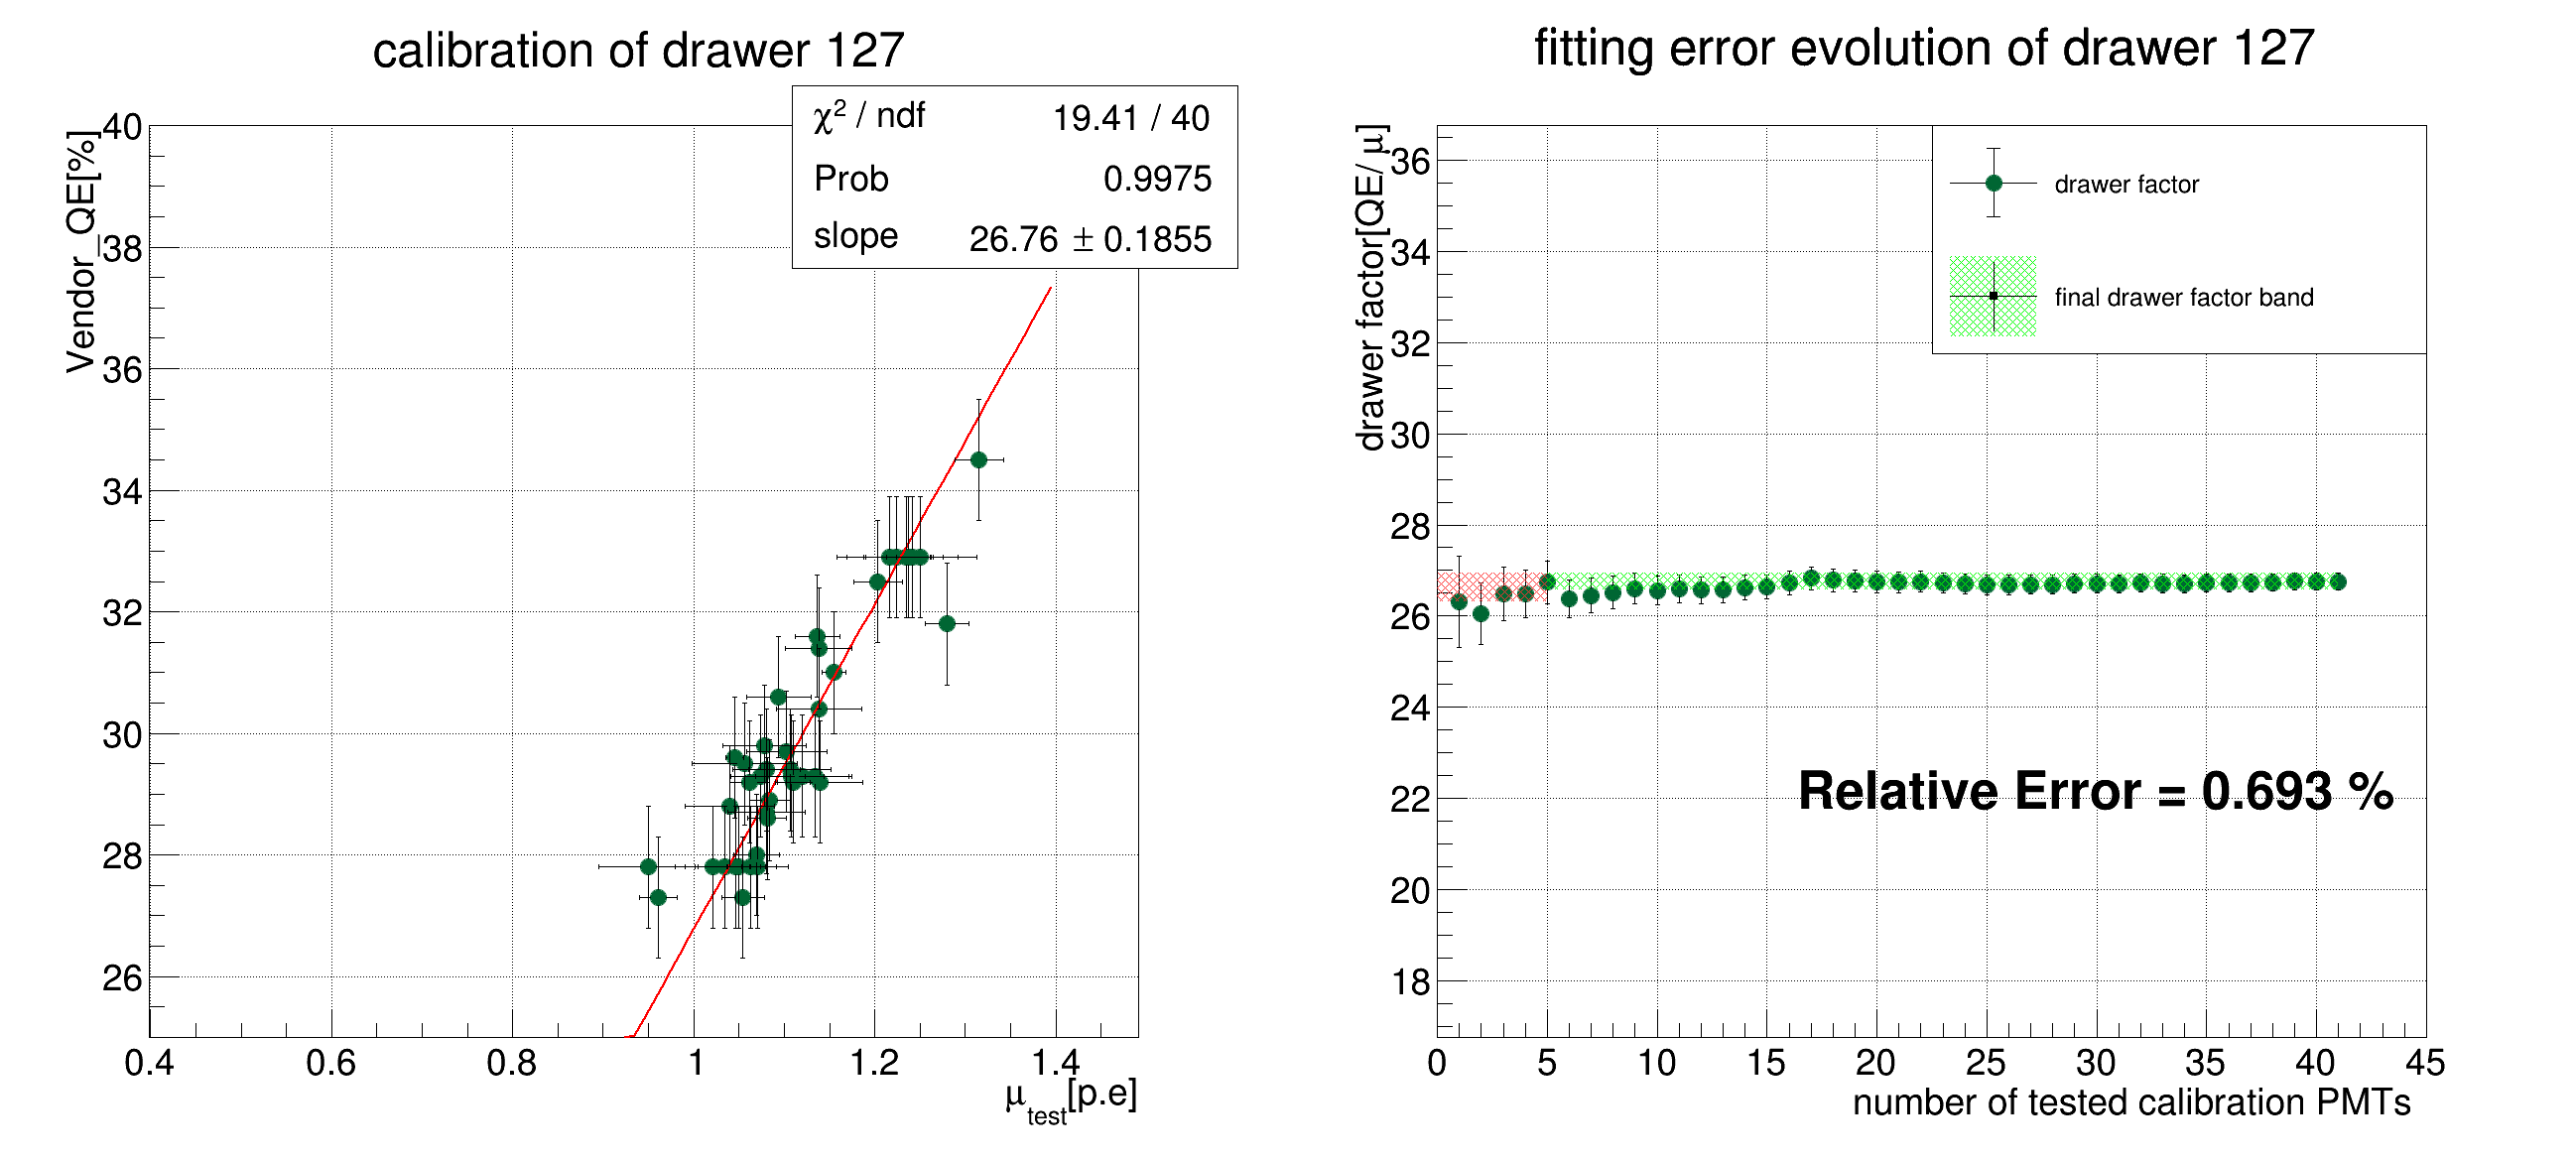
\includegraphics[width=0.45\textwidth]{sta101-26} 
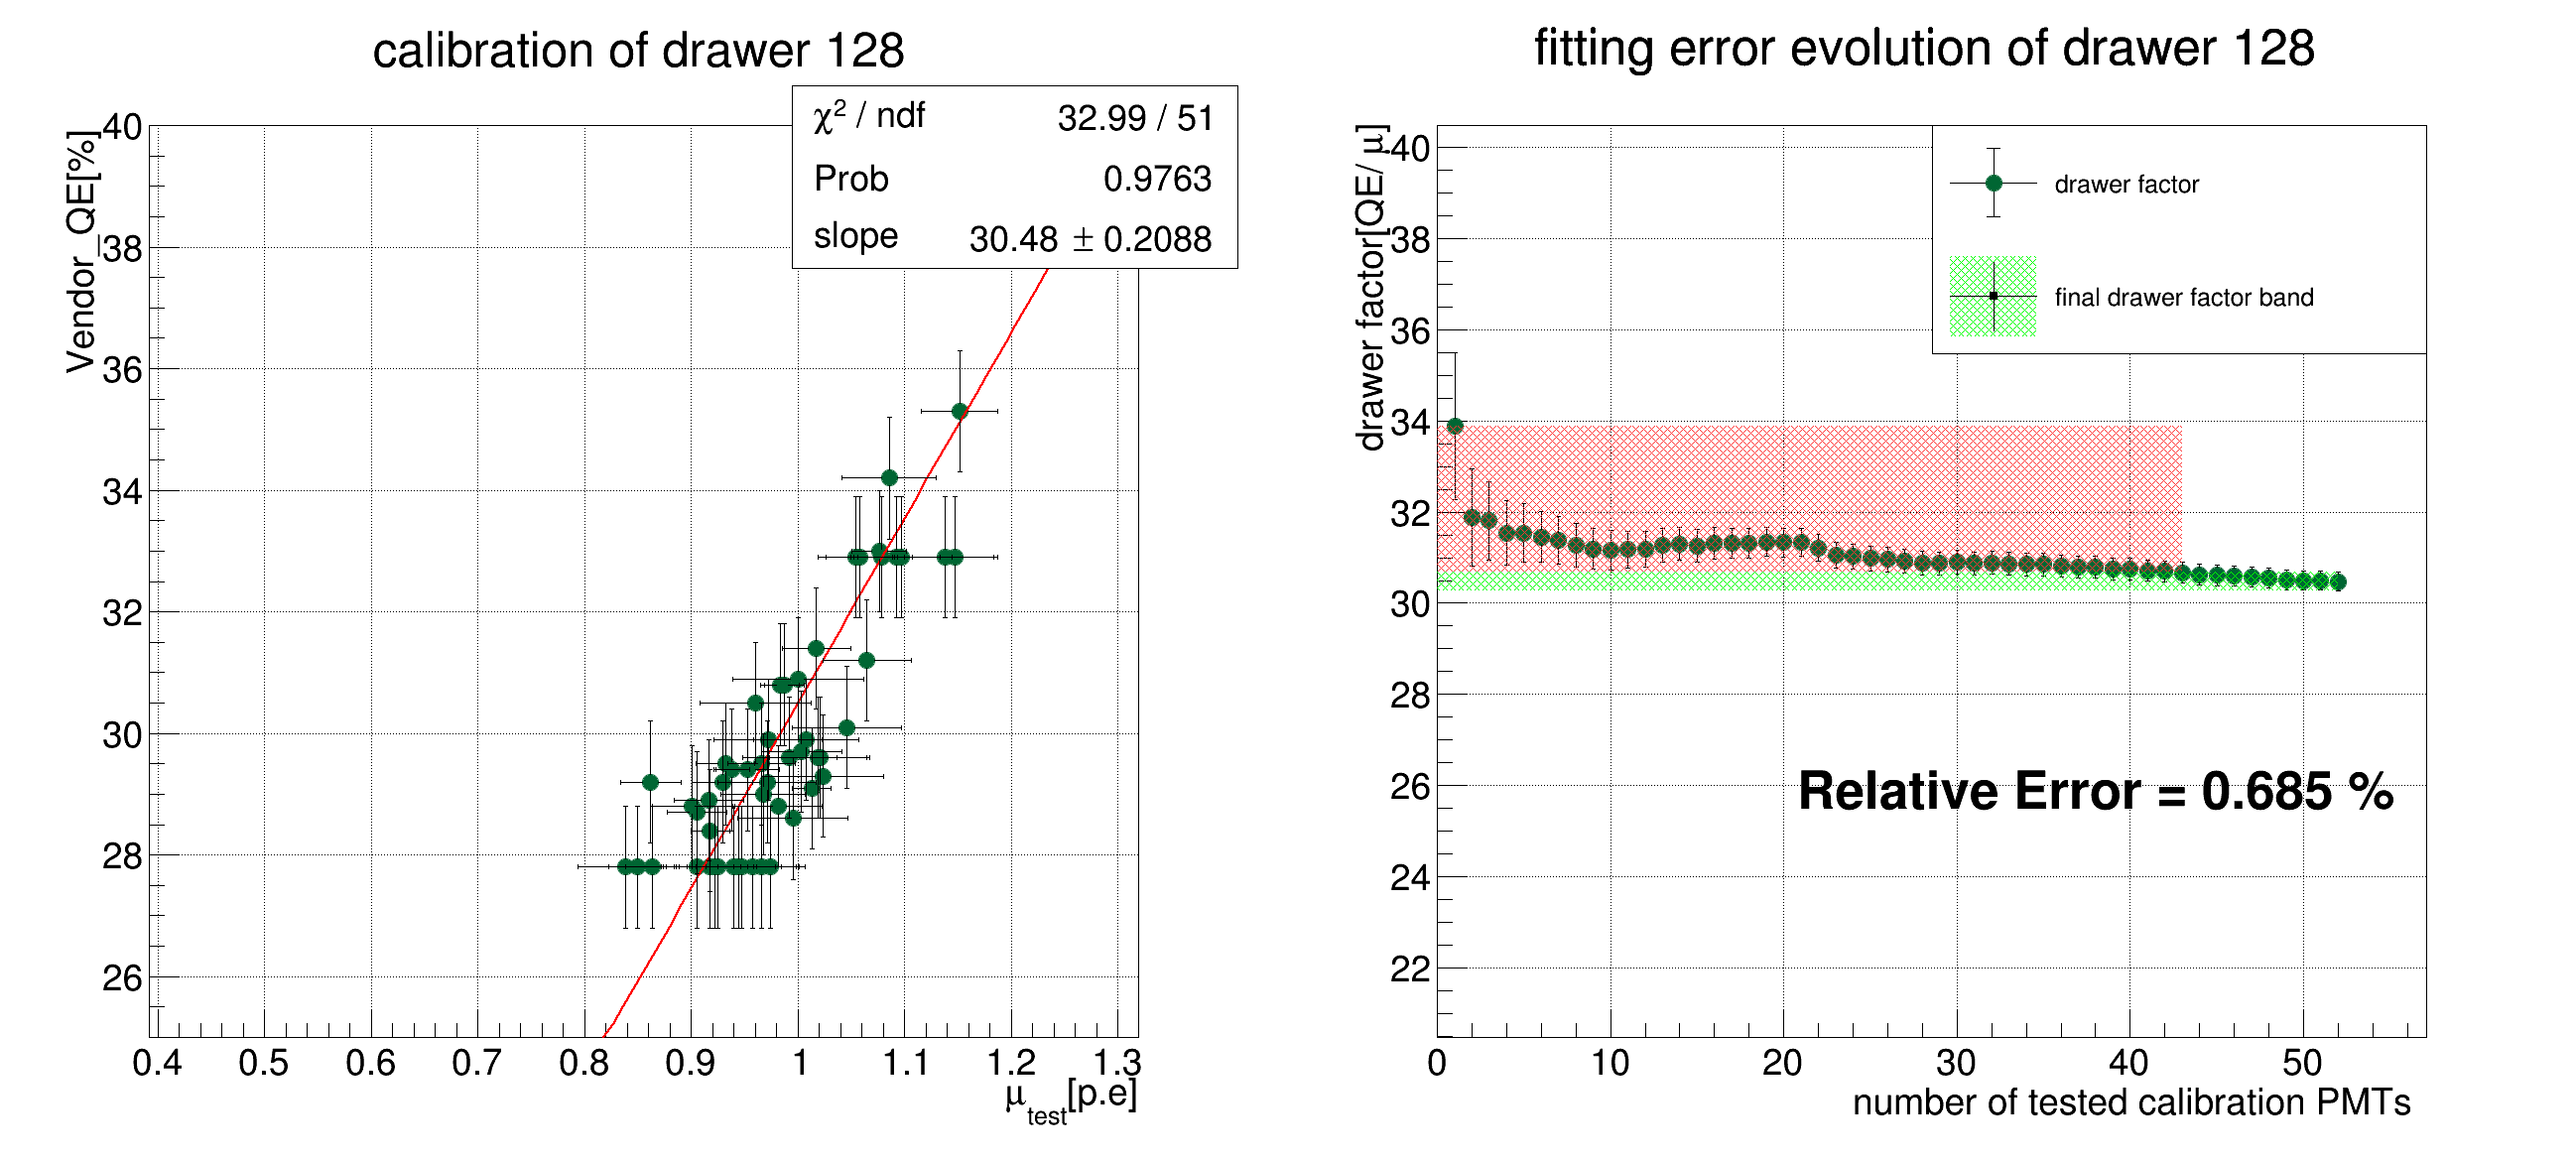
\includegraphics[width=0.45\textwidth]{sta101-27} 
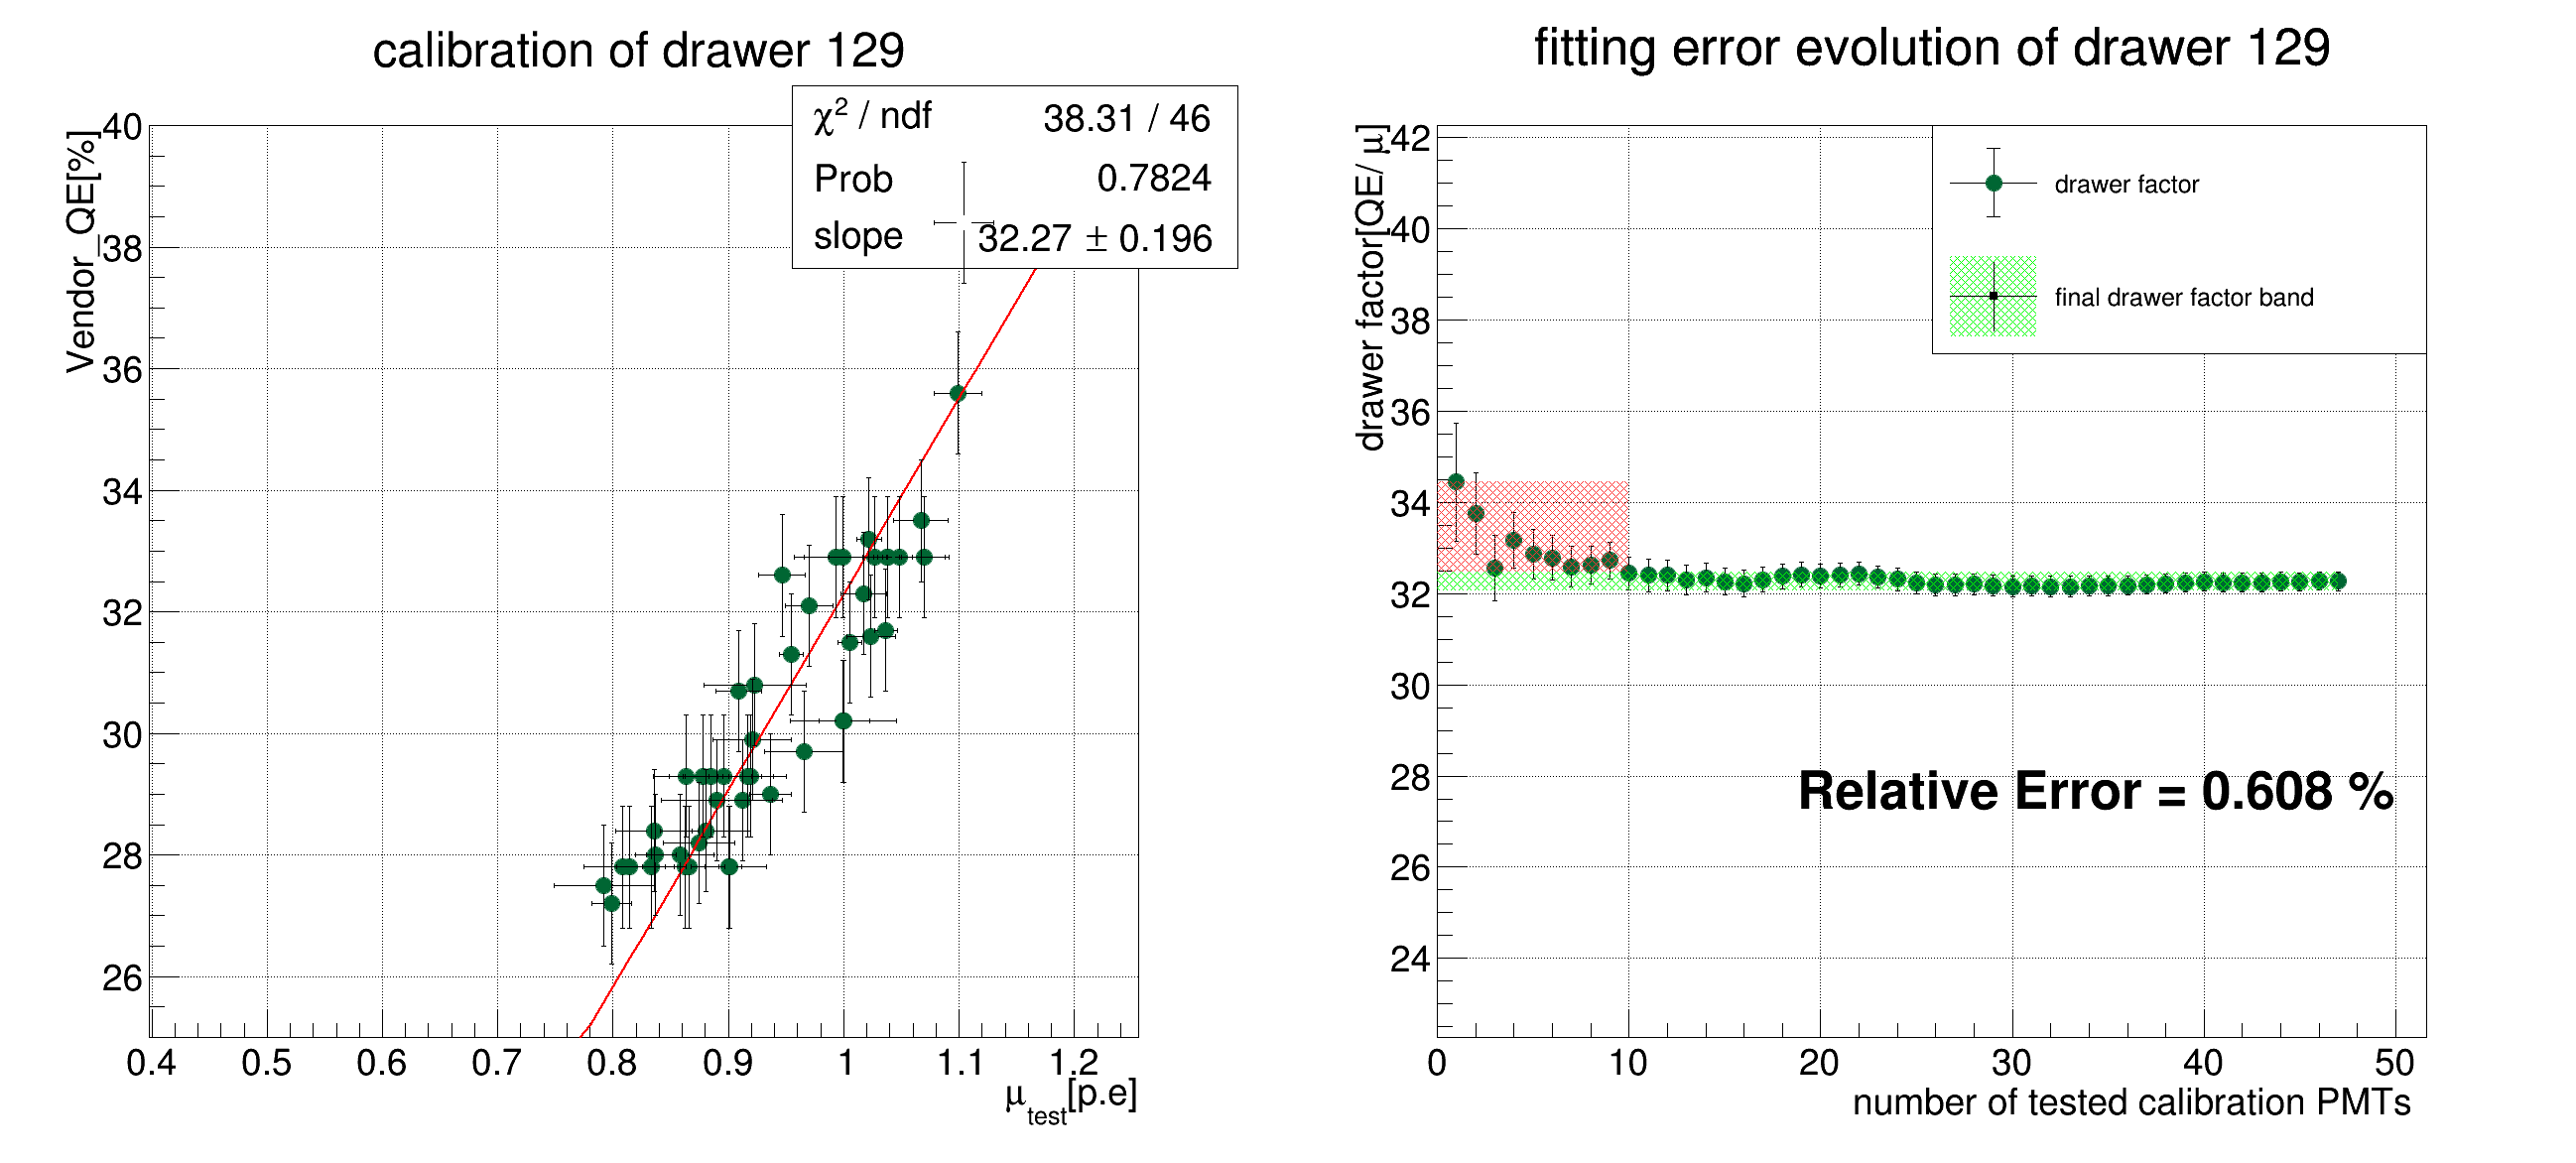
\includegraphics[width=0.45\textwidth]{sta101-28} 
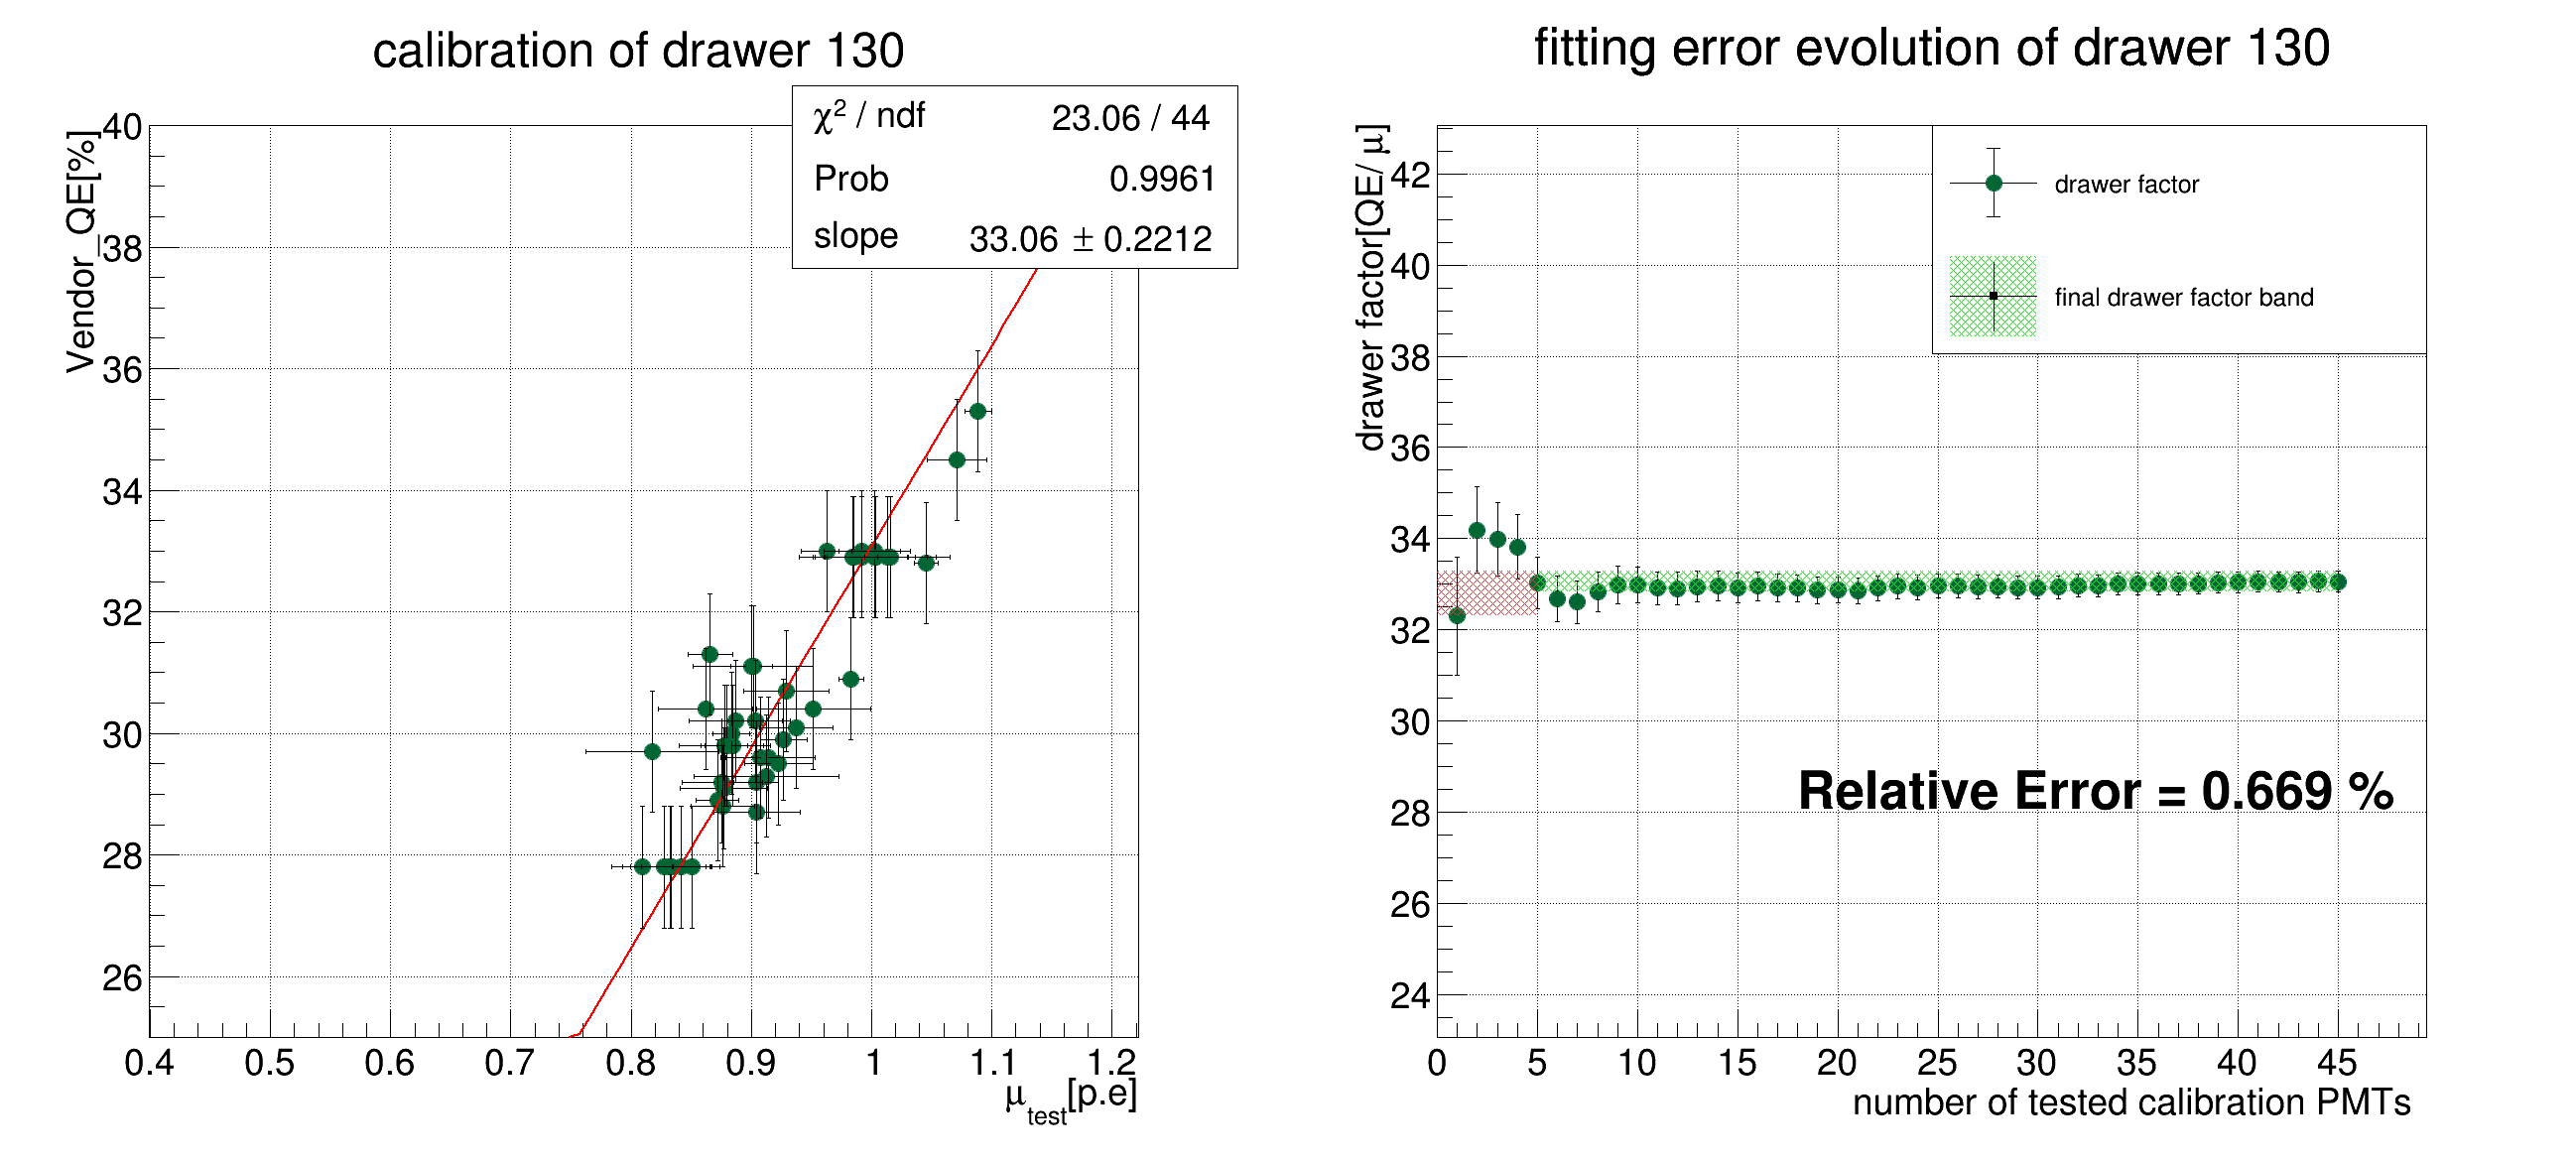
\includegraphics[width=0.45\textwidth]{sta101-29} 
\end{frame}
\begin{frame}{drawer-calibration}
\vspace{-.5cm}
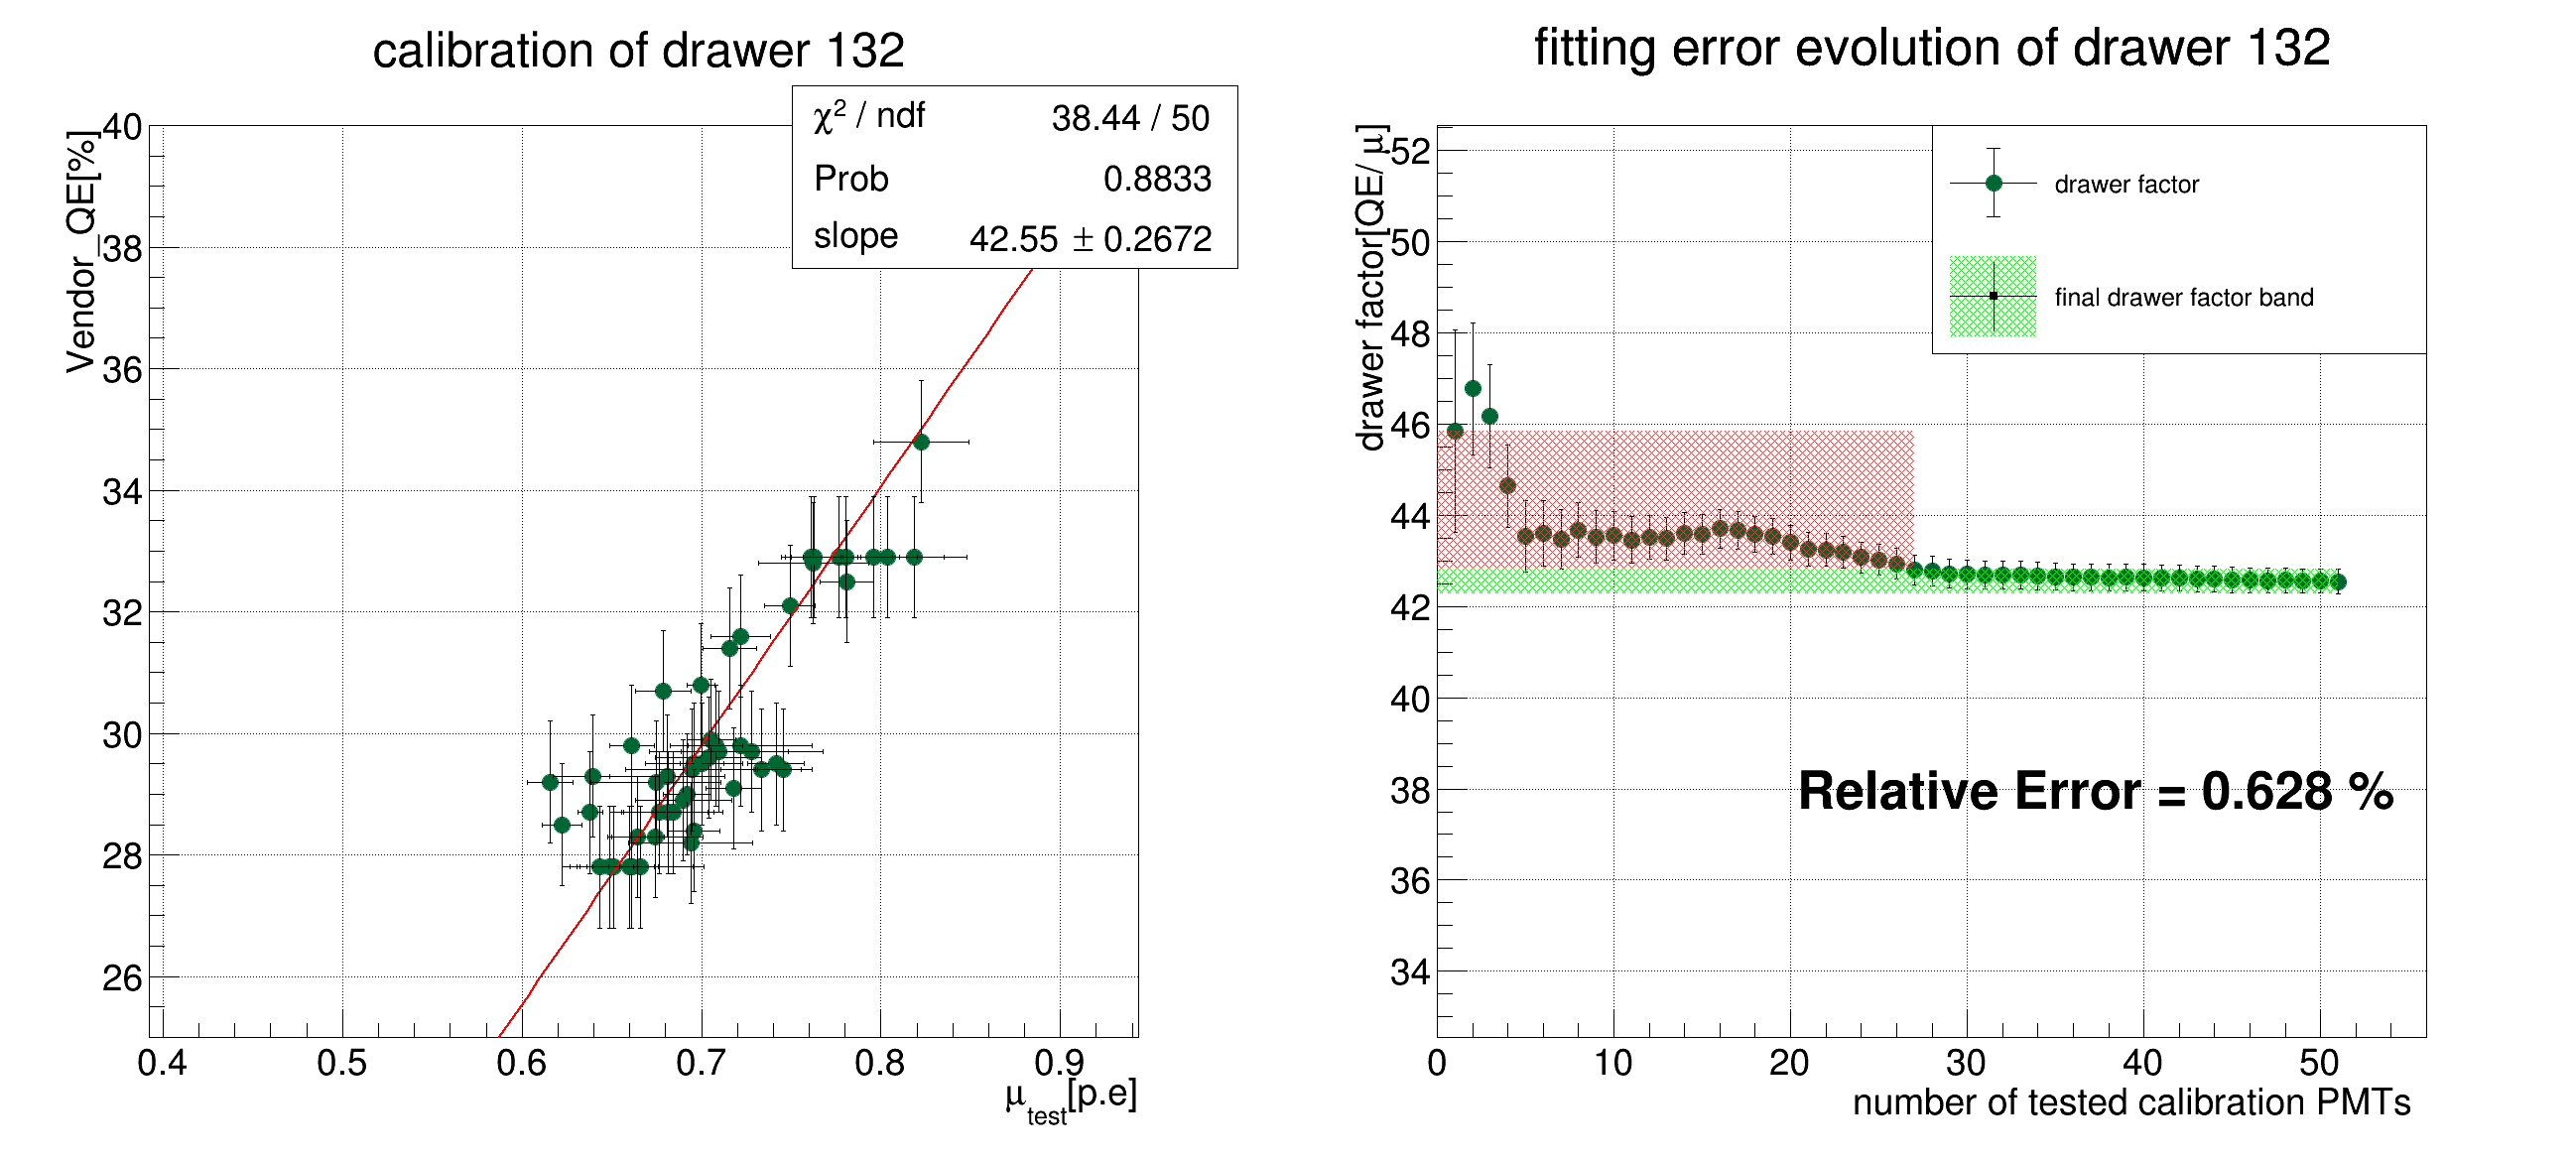
\includegraphics[width=0.45\textwidth]{sta101-30} 
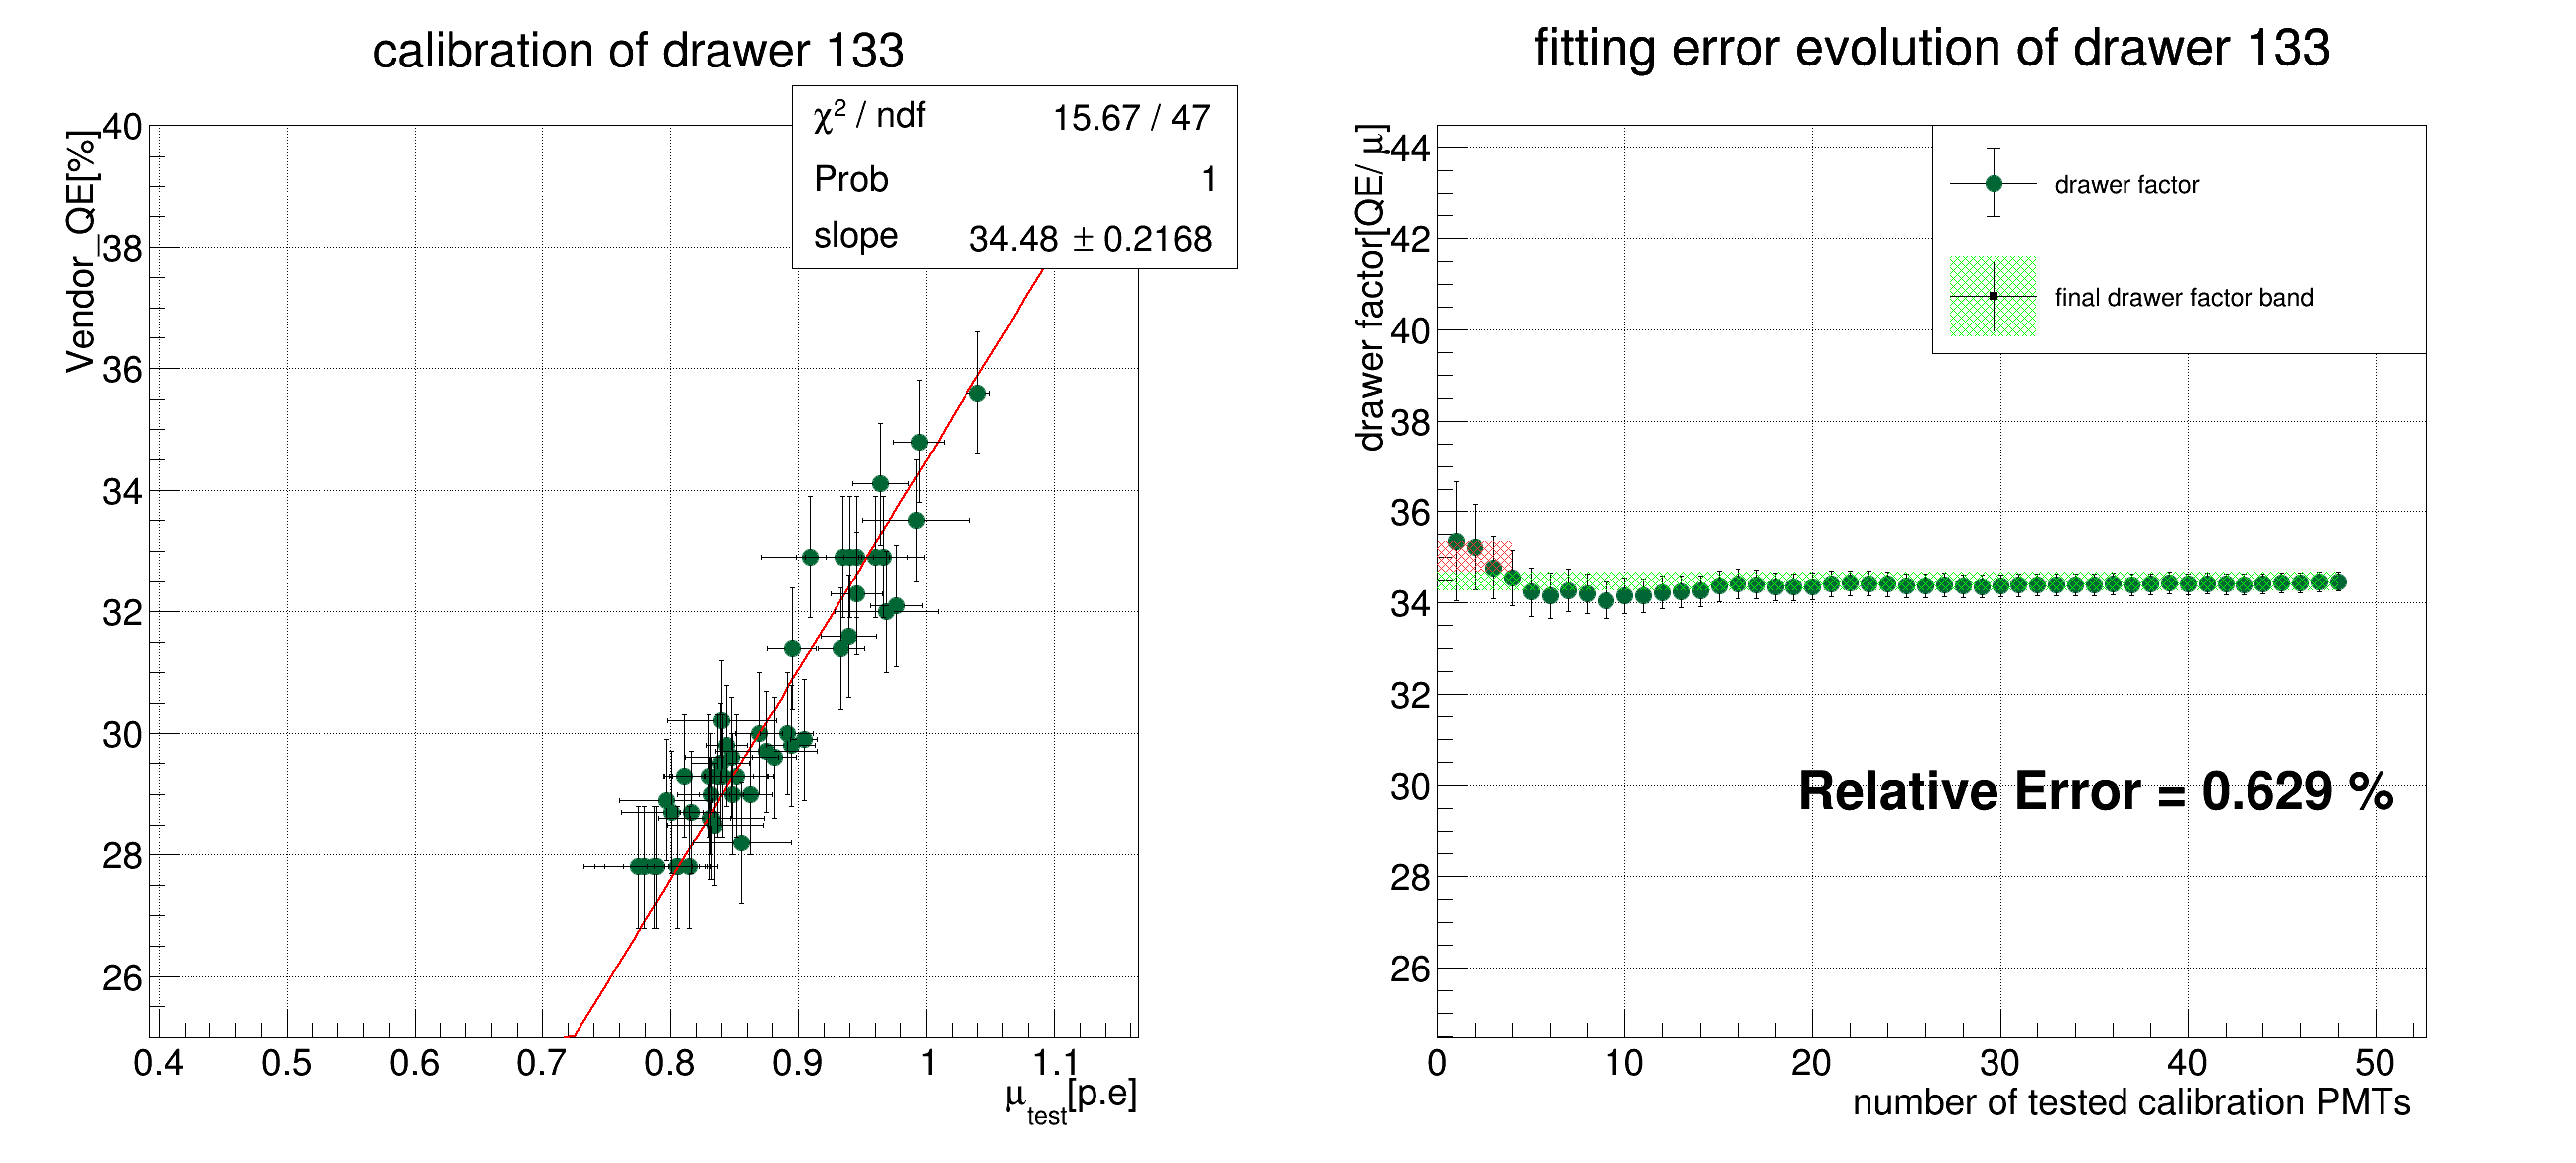
\includegraphics[width=0.45\textwidth]{sta101-31} 
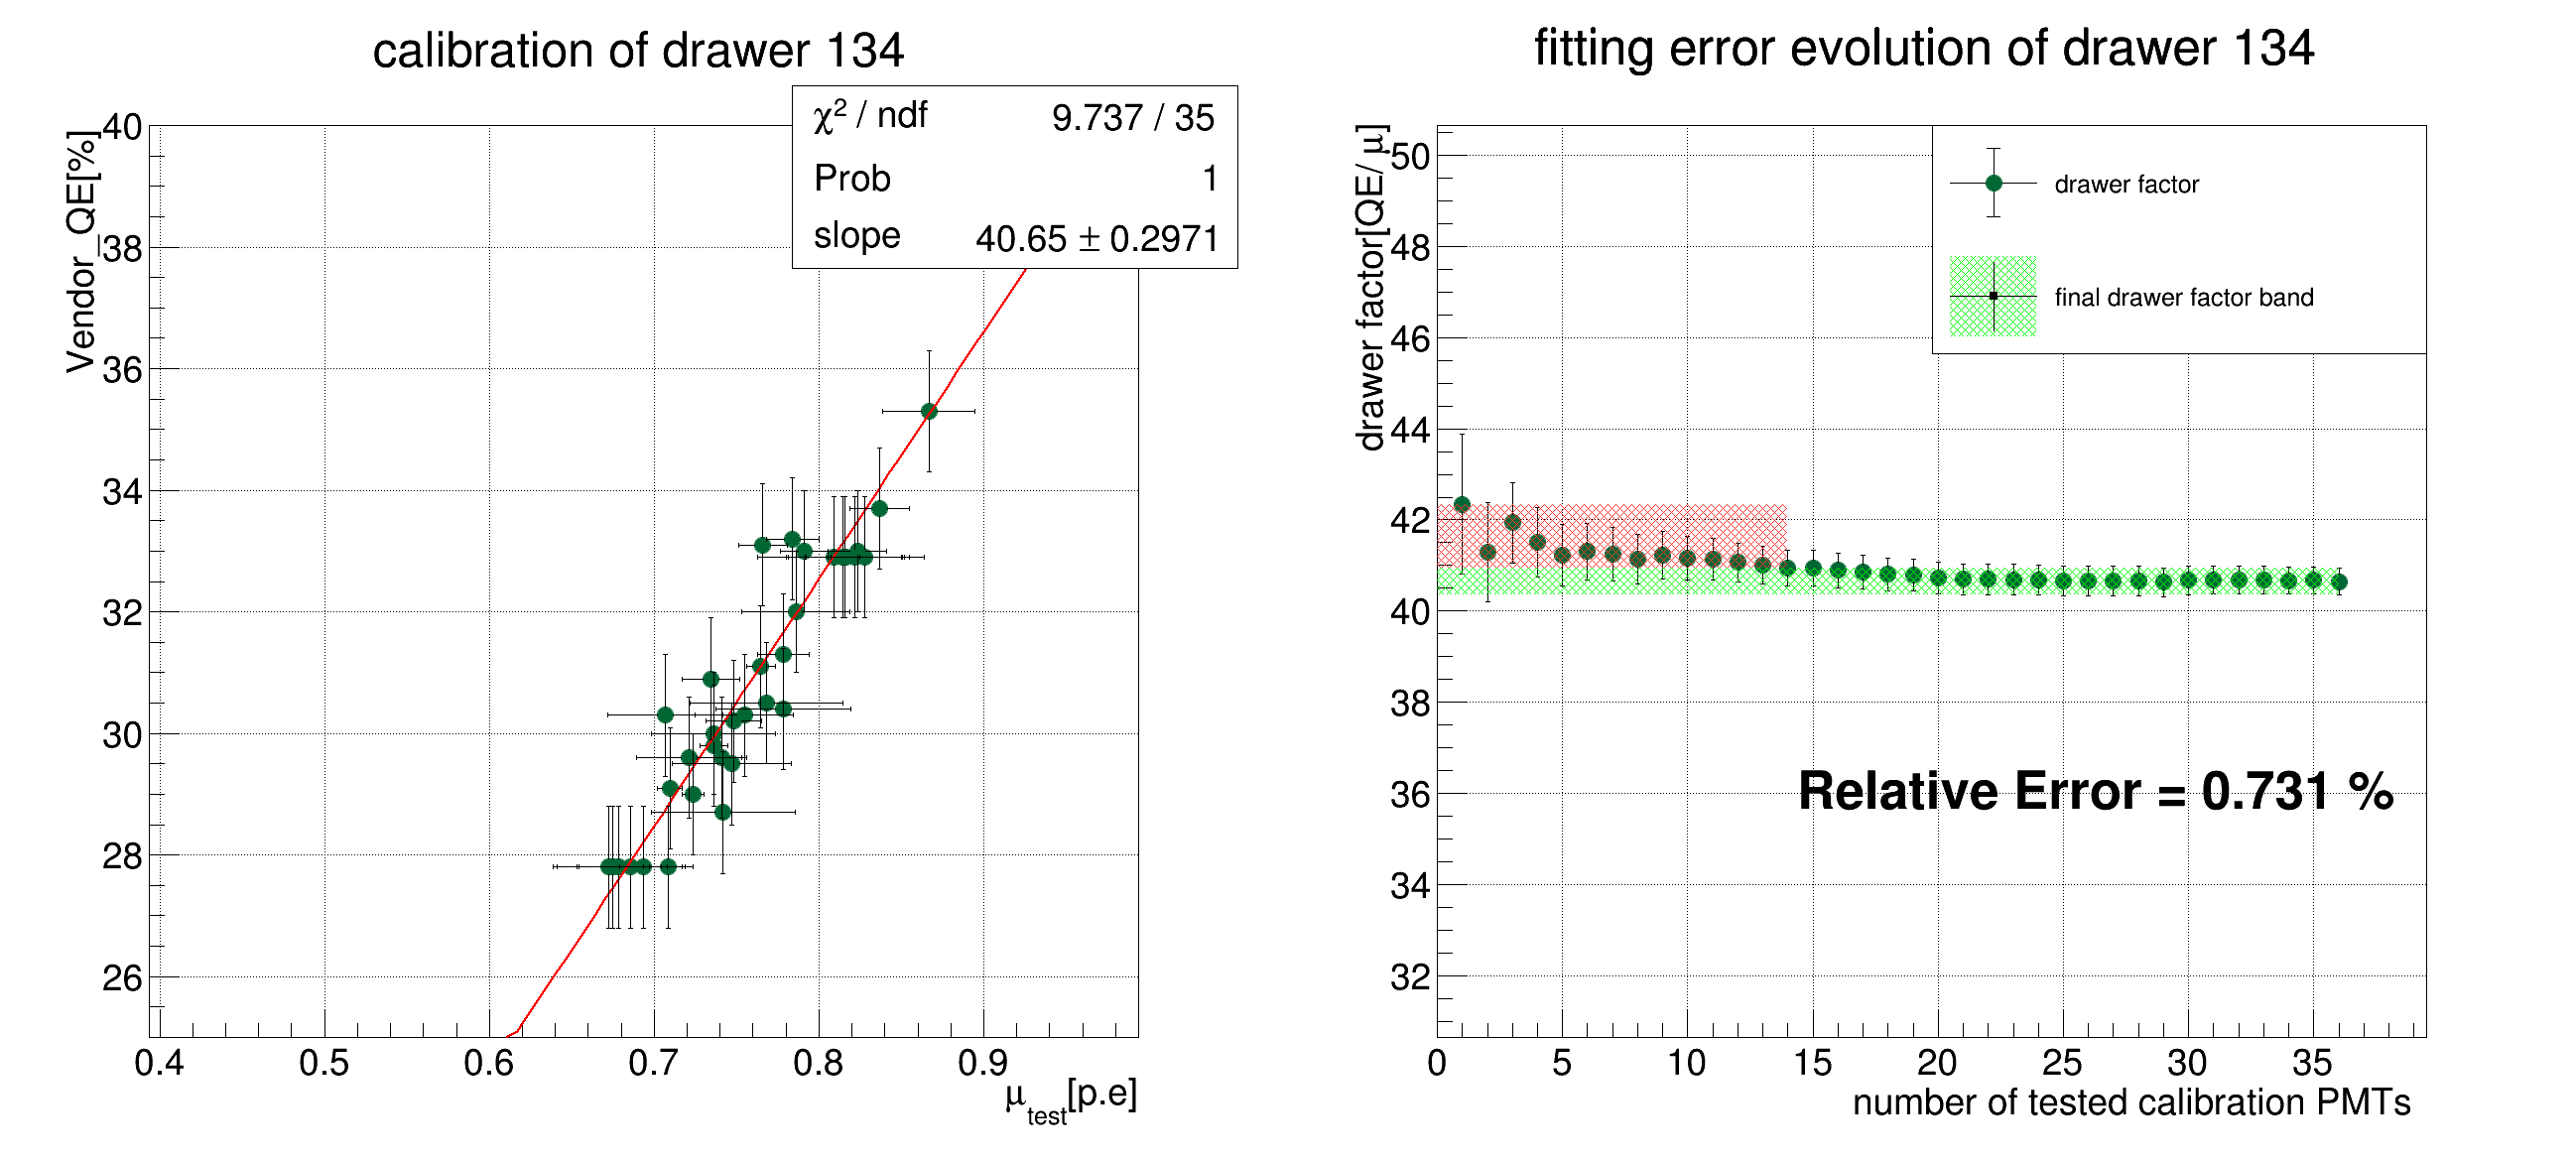
\includegraphics[width=0.45\textwidth]{sta101-32} 
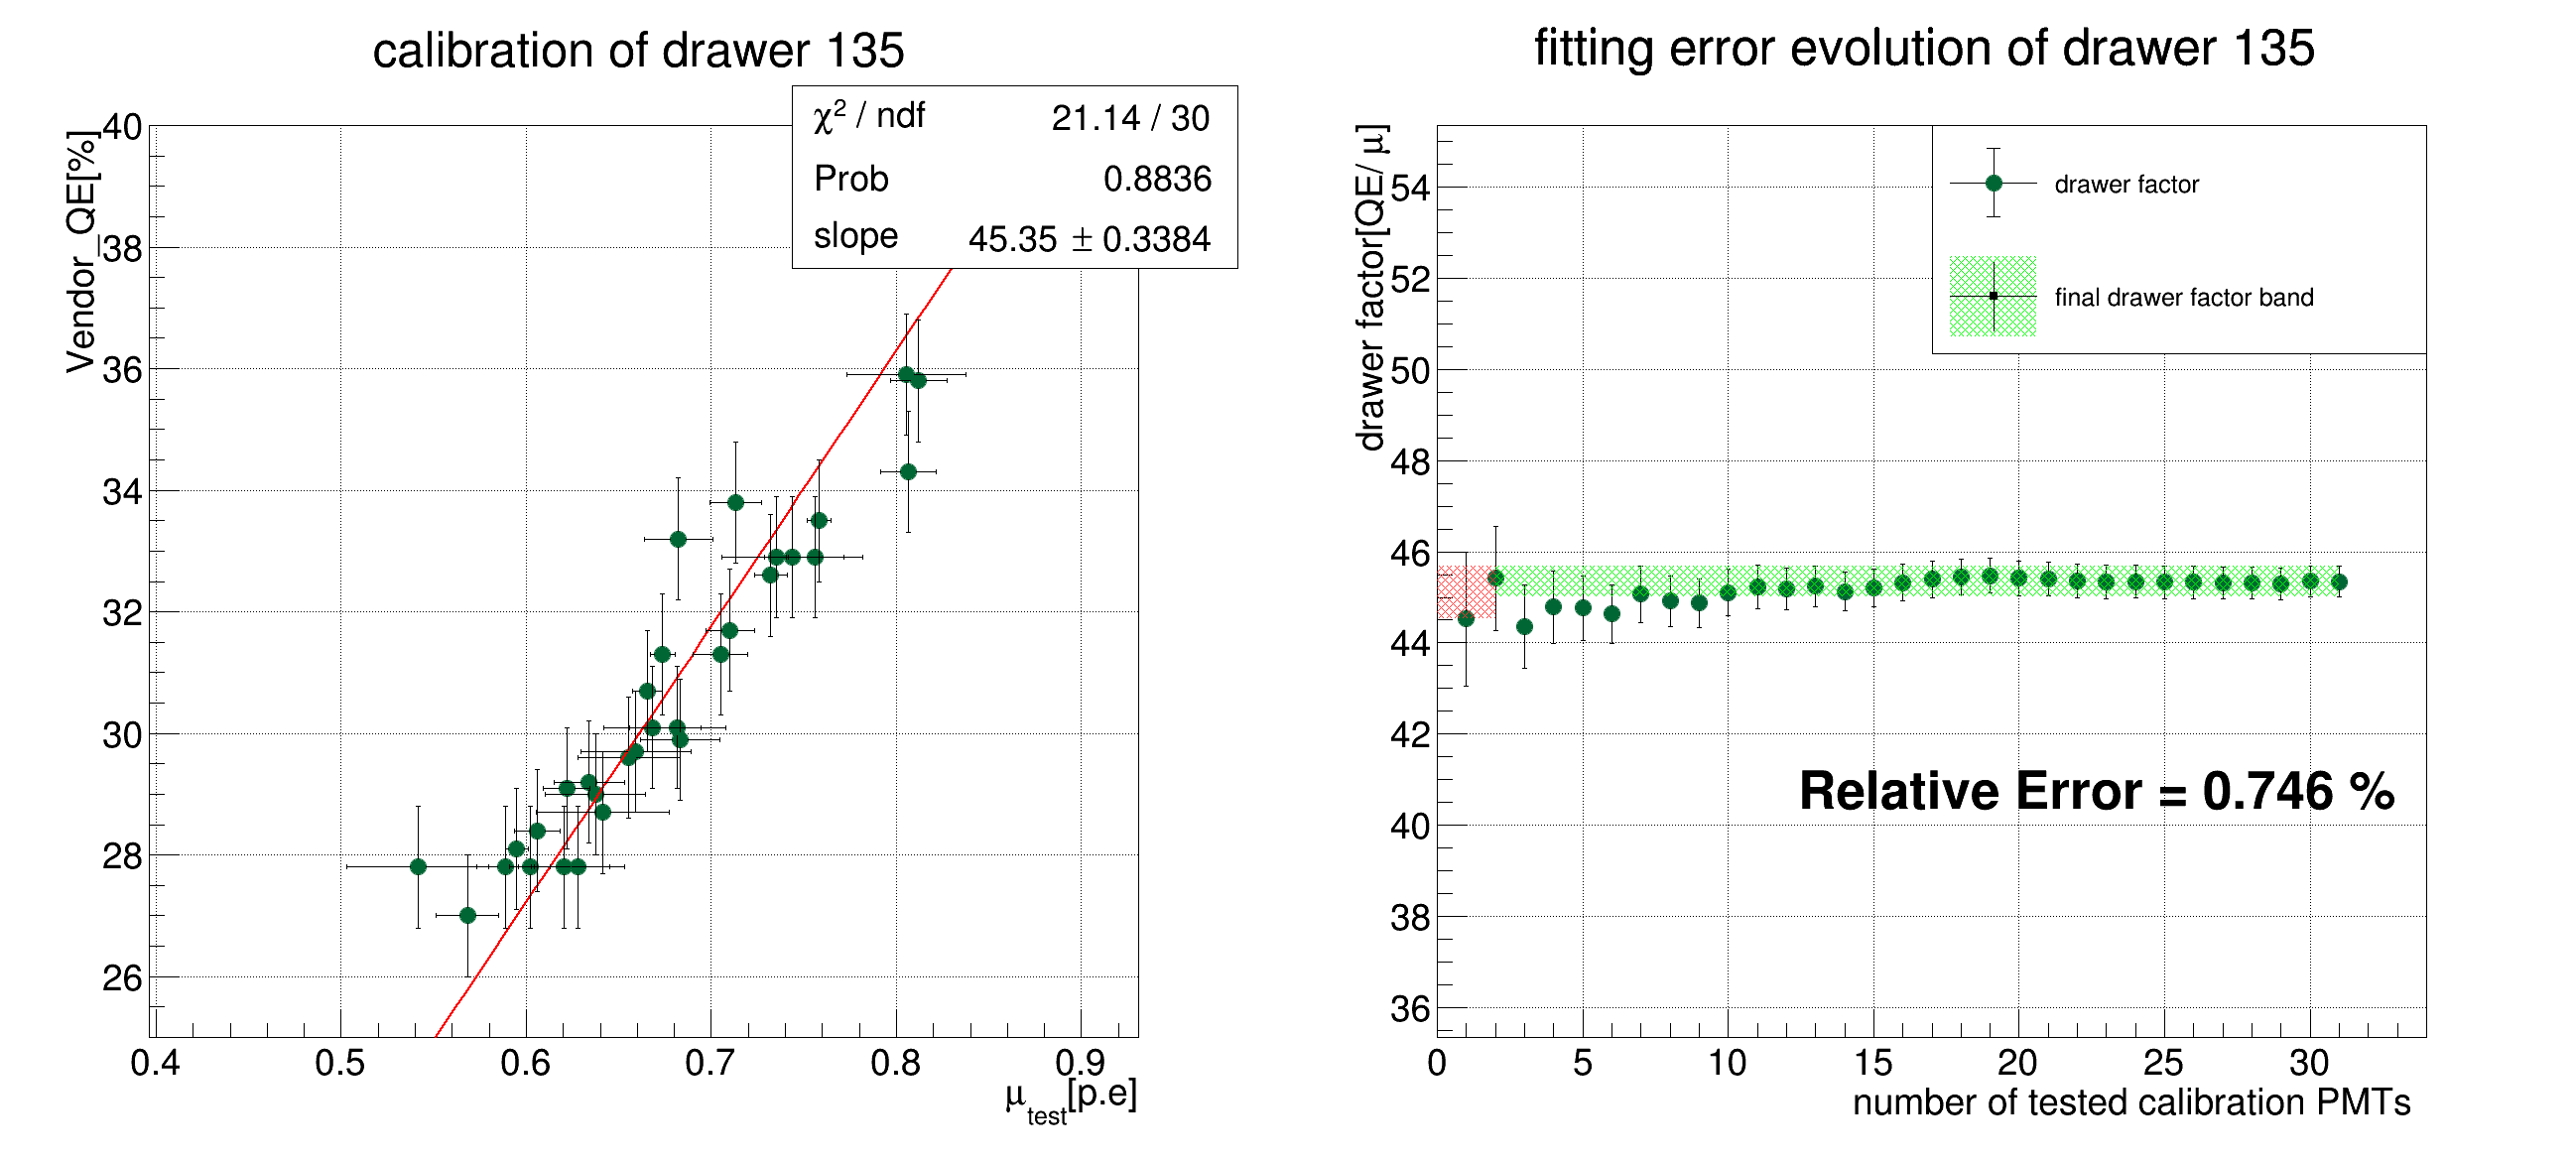
\includegraphics[width=0.45\textwidth]{sta101-33} 
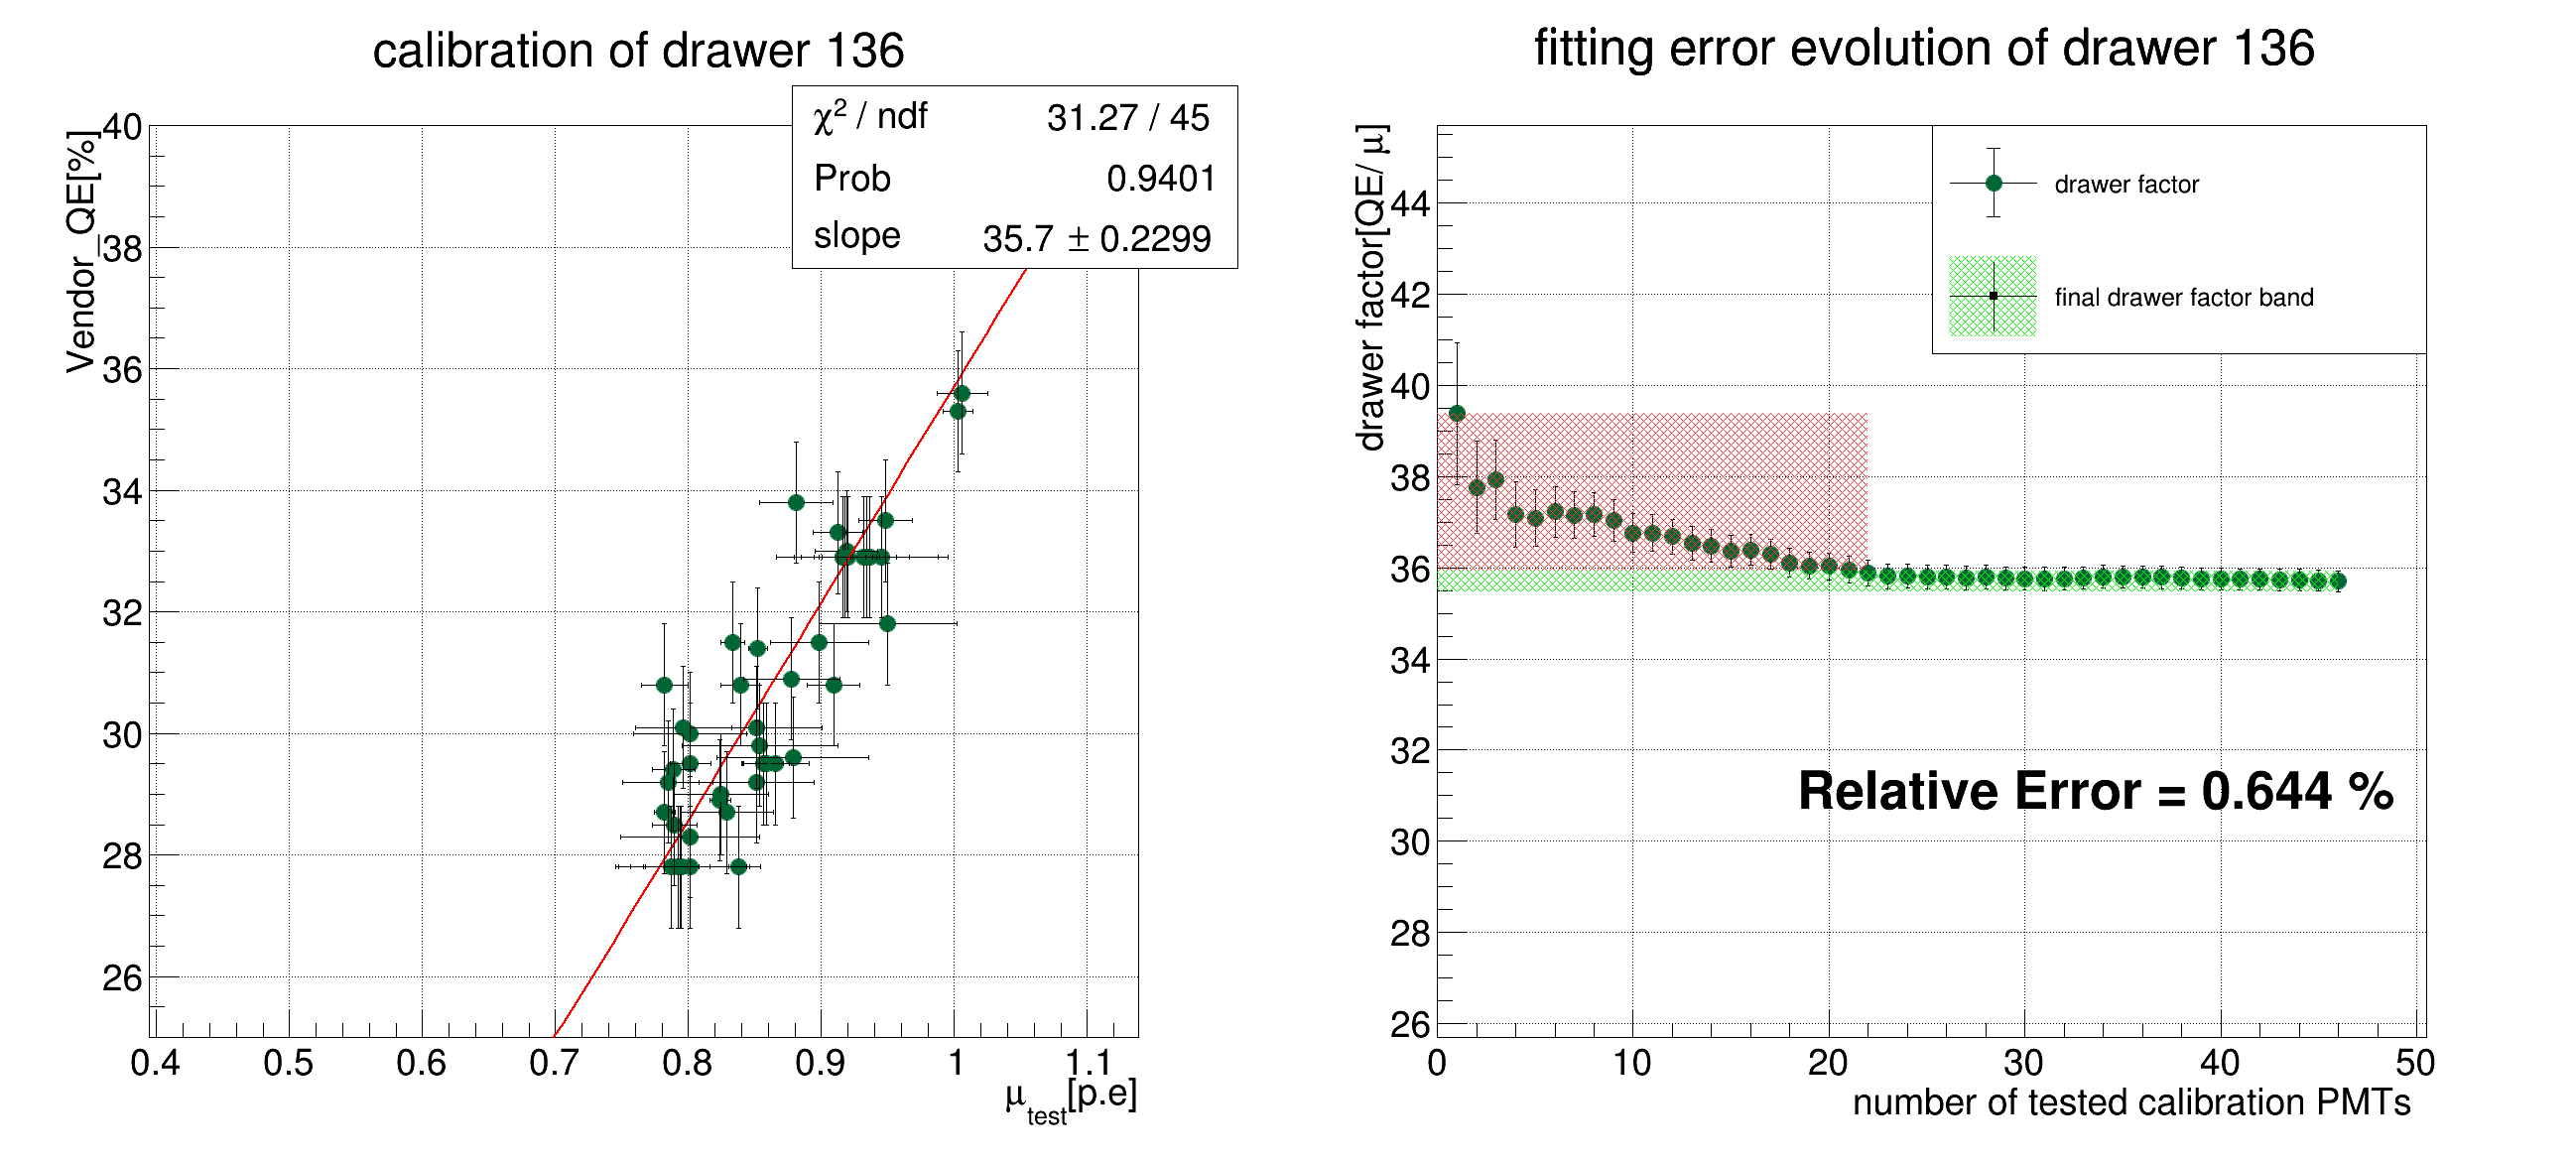
\includegraphics[width=0.45\textwidth]{sta101-34} 
\end{frame}
%%%%%%%%%%%%%%%%%%%%%%%%%%%%%%%%%%%%%%%%%
\begin{frame}{comparasion of drawer factor}
factor\_1 is my result, factor\_2 is onsite result\footnote{$y=1.148x+0.998$}.
\vspace{-.05cm}
\begin{figure}
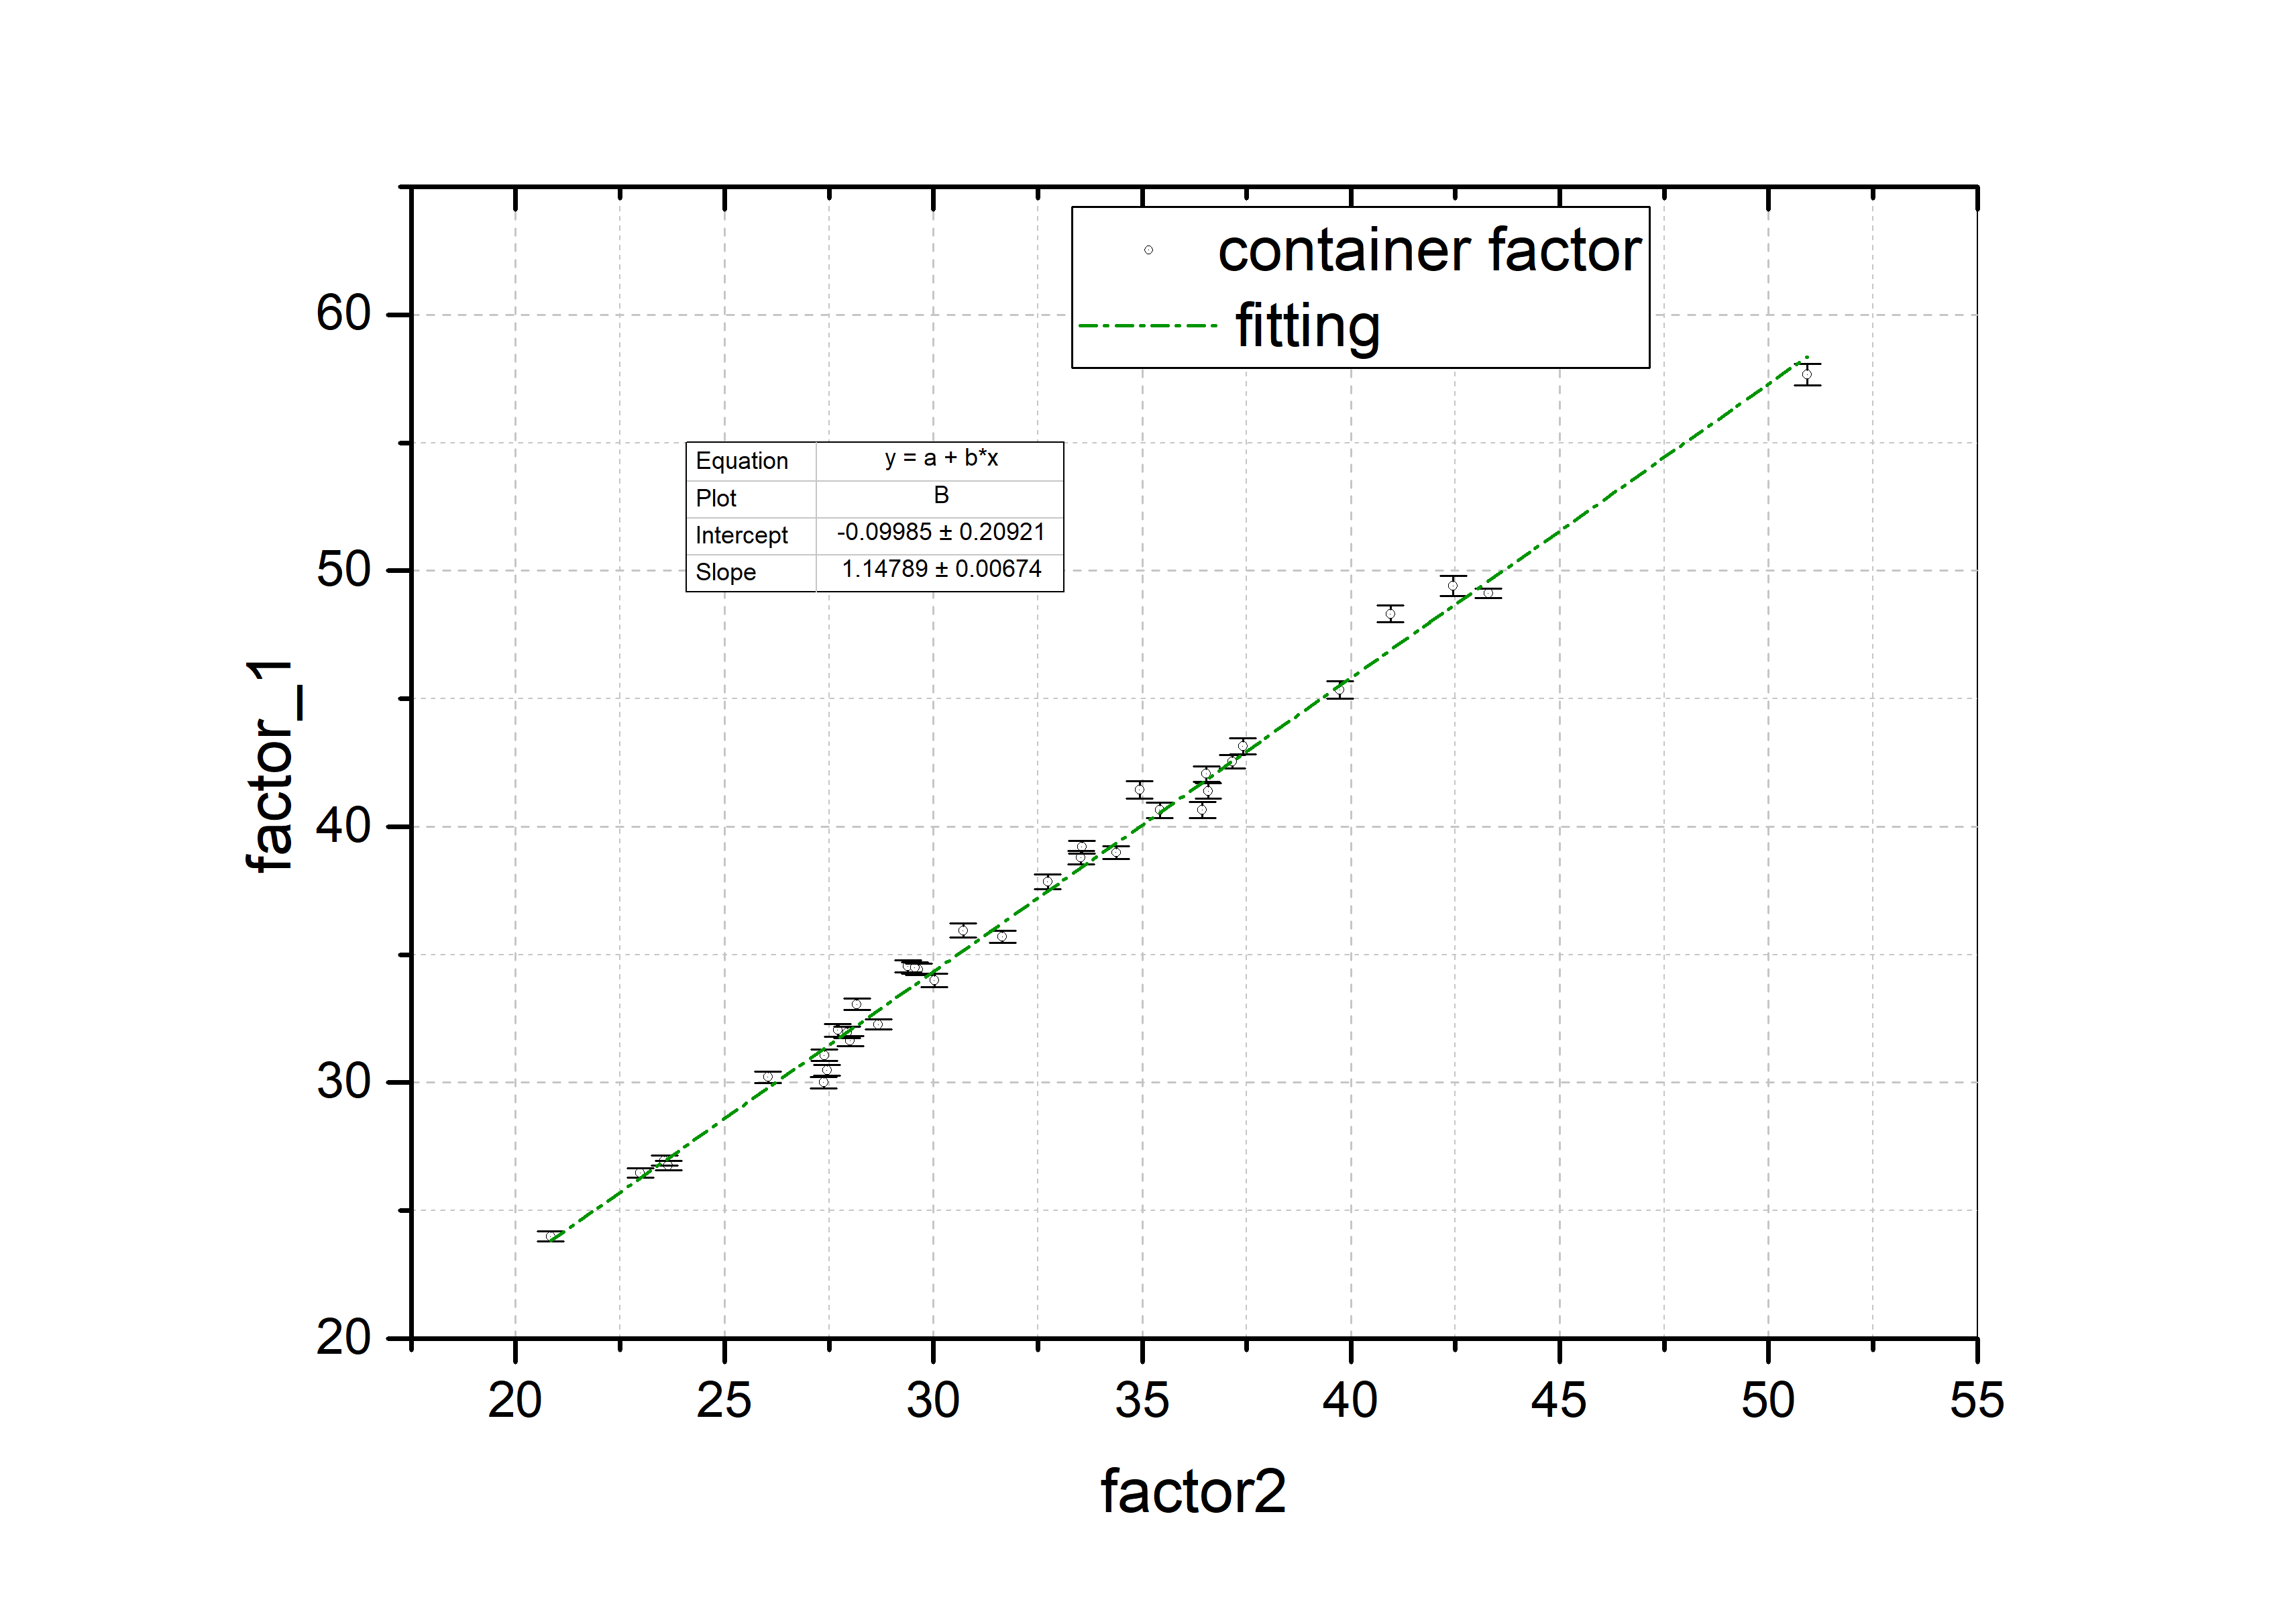
\includegraphics[width=0.72\textwidth]{drawerfactors} 
%\caption{comparasion of drawer factor}
\end{figure}
\end{frame}

\begin{frame}{correlation of results from two system}
fitting $PDE_c$ and $PDE_s$ for high-QE MCP PMTs.
\begin{figure}
\centering
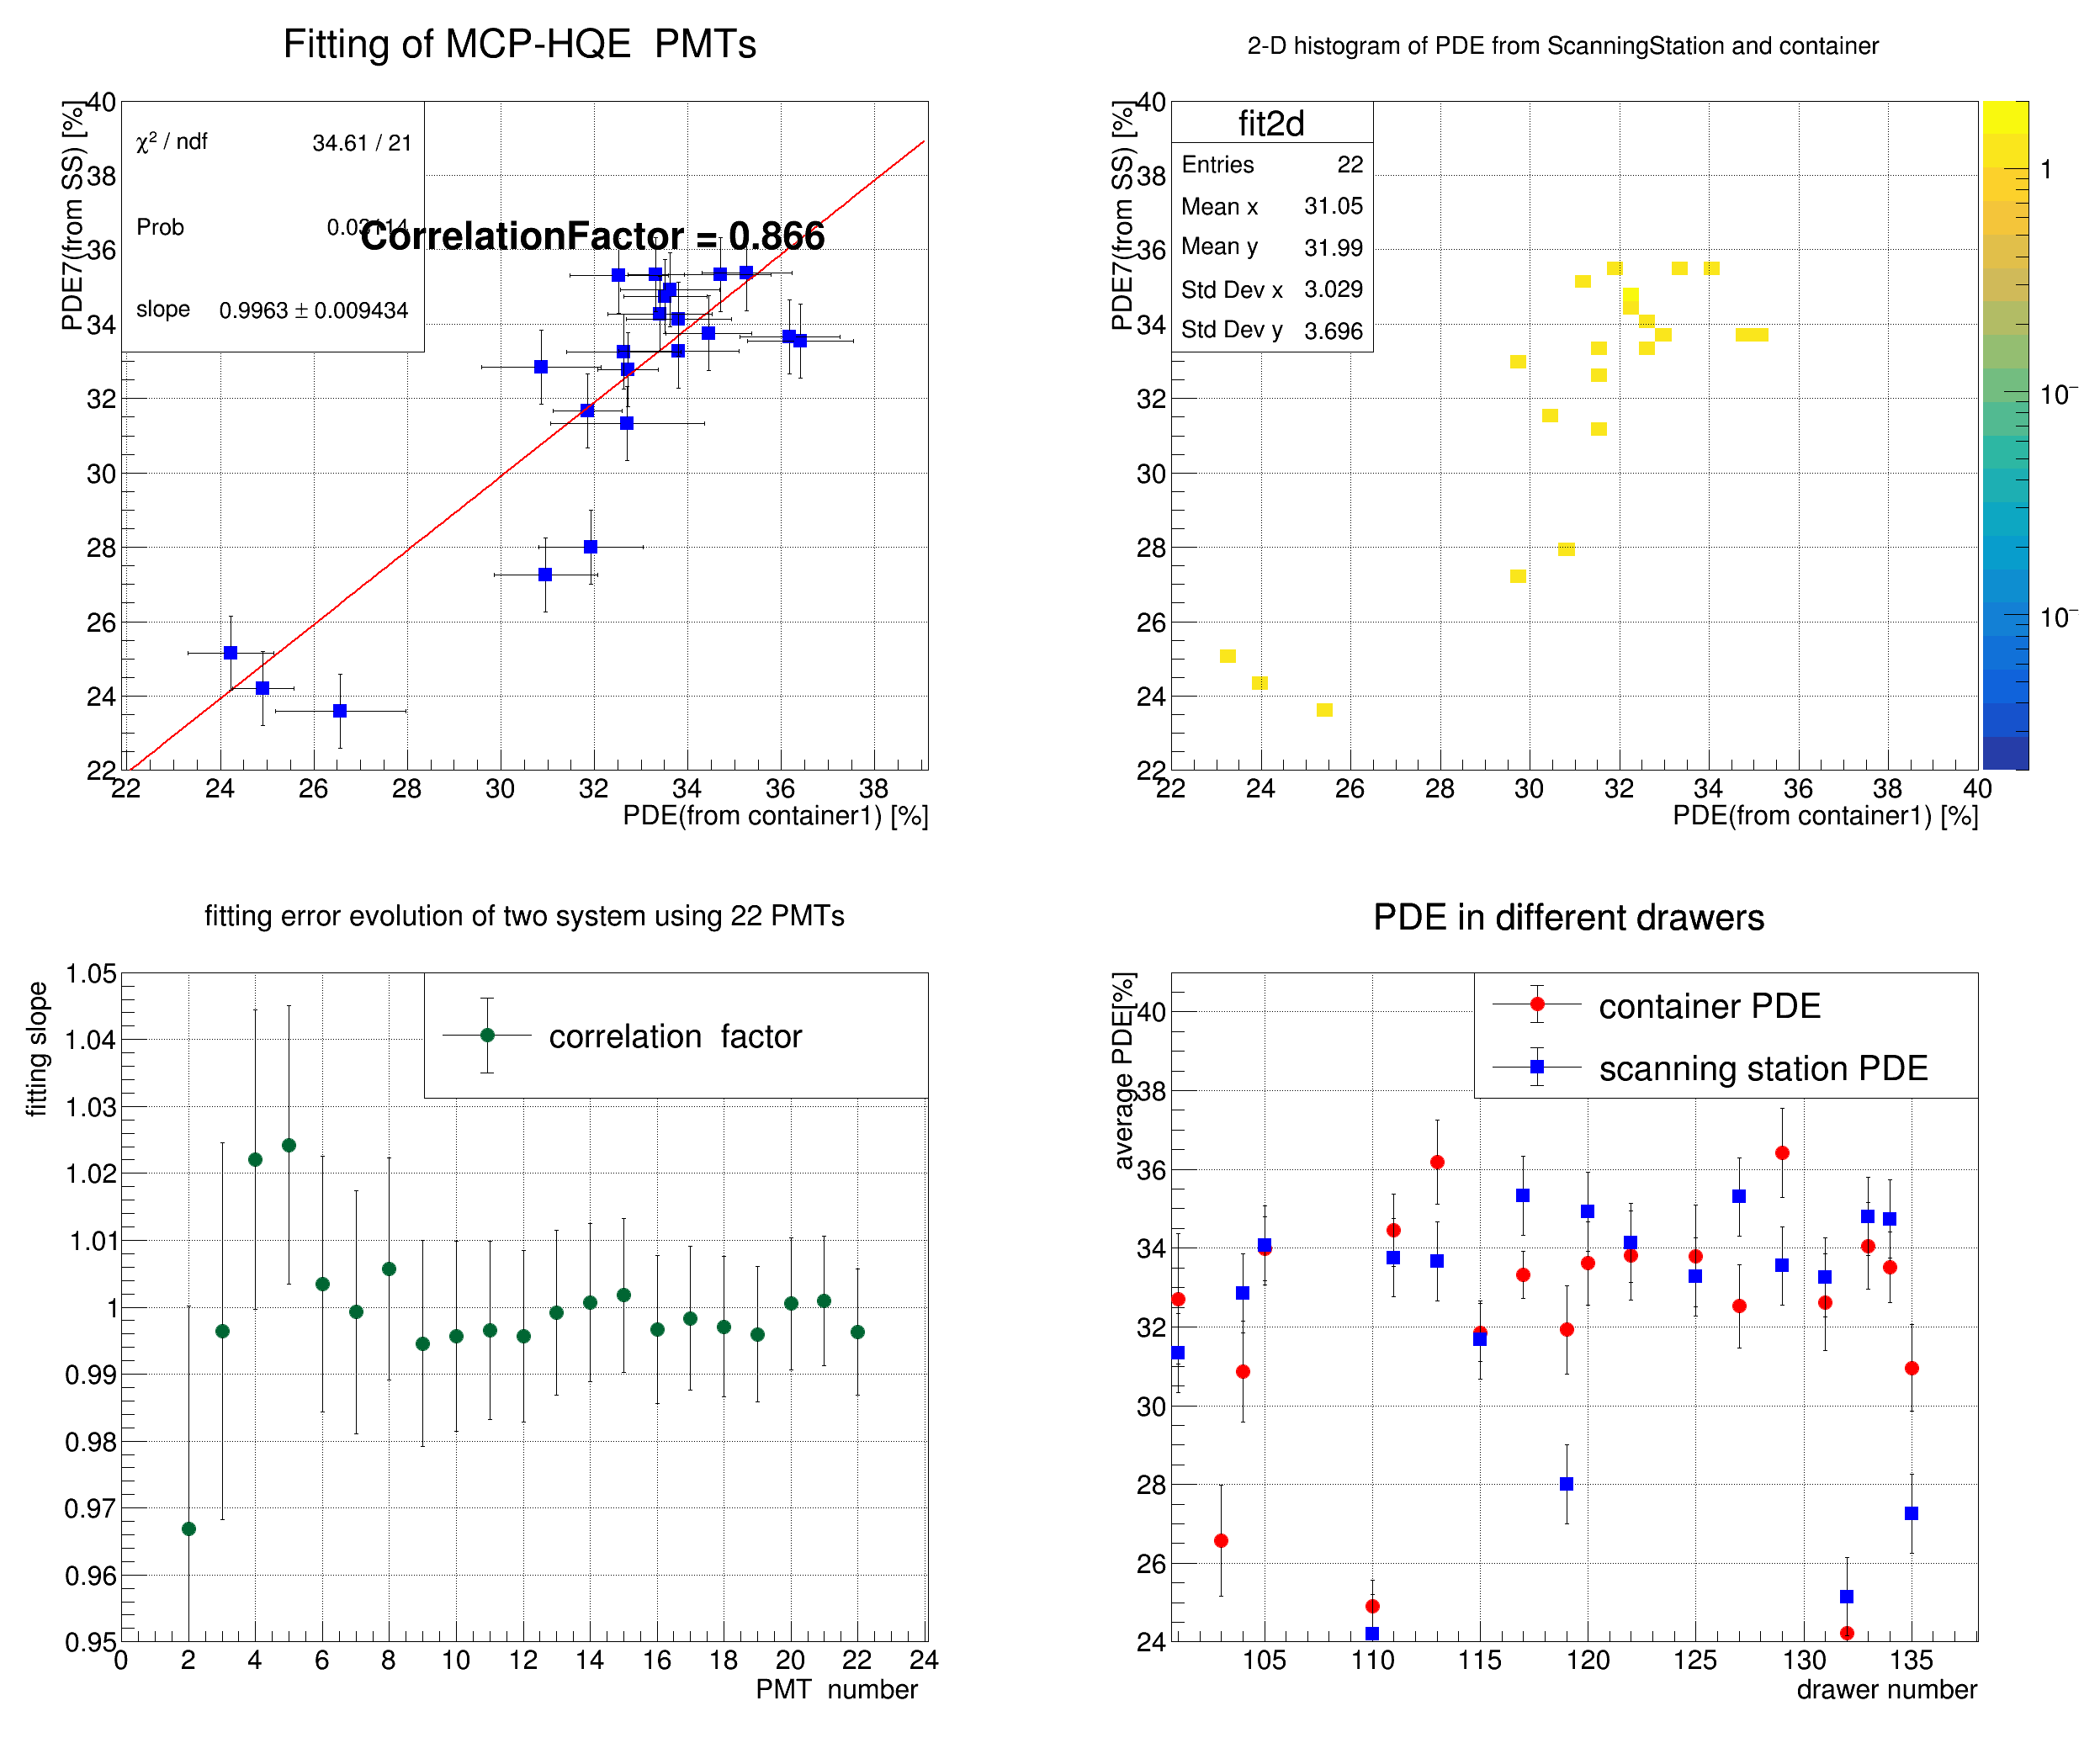
\includegraphics[width=0.68\textwidth]{fit_mcp_hqe_noint}
\end{figure}
\end{frame}
%\begin{frame}{两套装置测量结果的转换}
\begin{frame}{correlation of results from two system}
fitting $PDE_c$ and $PDE_s$ for low-QE PMTs.
%利用i$PDE_c$和$PDE_s$对所有低量子效率MCP-PMT拟合$f_{cs}$的结果:
\begin{figure}
\centering
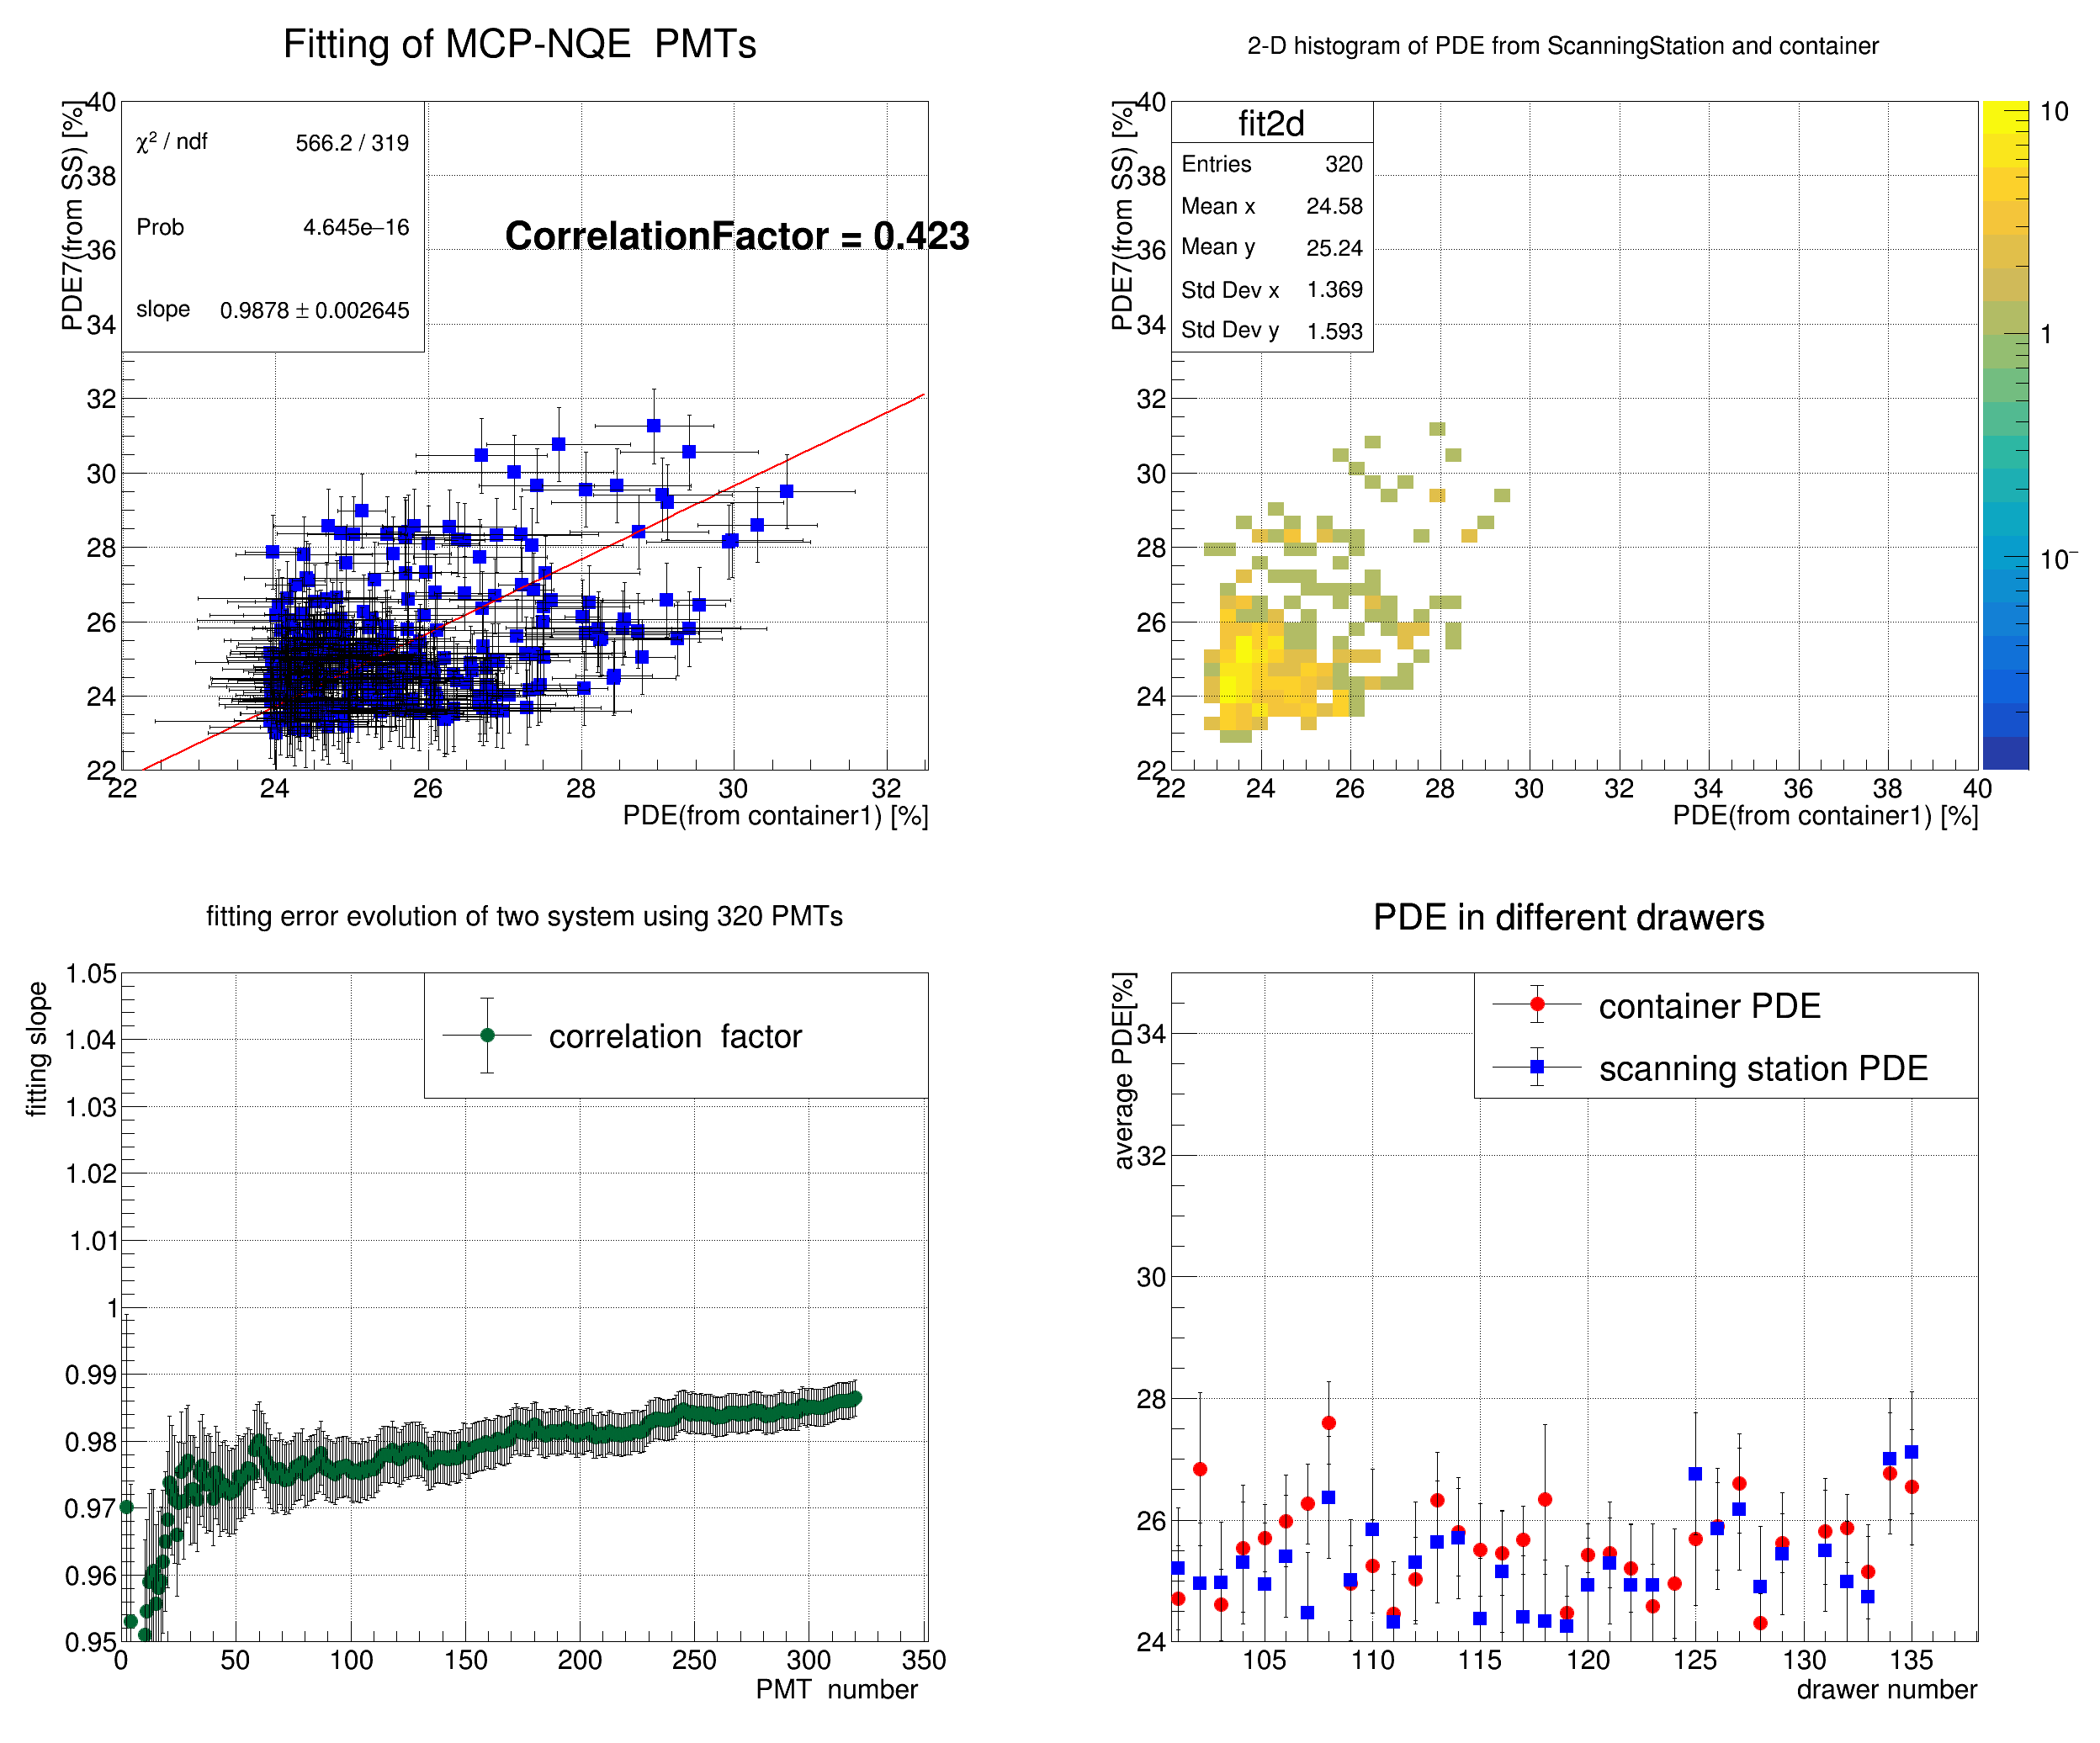
\includegraphics[width=0.68\textwidth]{fit_mcp_nqe_noint}
\end{figure}
\end{frame}
%%%%%%%%%%%%%%%%%%%%%%%%%%%%%%%%%%%%%%%%%%%
\begin{frame}{PDE of reference PMTs}
\begin{figure}
\centering
\includegraphics[width=0.68\textwidth]{ref_sta}
\end{figure}
\end{frame}
%%%%%%%%%%%%%%%%%%%%%%%%%%%%%%%%%%%%%%%%%%%
\begin{frame}{HV of reference PMTs}
%新DAQ对系统的性能产生了影响,高压平均值发生了变化:
\begin{figure}
\centering
\includegraphics[width=0.68\textwidth]{ref_HV_sta}
\end{figure}
\end{frame}
%%%%%%%%%%%%%%%%%%%%%%%%%%%%%%%%%%%%%%%%%%%
\begin{frame}{EA0419}
The reference PMT EA0419 was kept in drawer101:
\begin{figure}
\centering
\includegraphics[width=0.98\textwidth]{101_sta}
\end{figure}
\end{frame}
%%%%%%%%%%%%%%%%%%%%%%%%%%%%%%%%%%%%%%%%%%%
\begin{frame}{DCR}
\begin{figure}
\centering
\includegraphics[width=0.48\textwidth]{vendordcr_mcp}
\includegraphics[width=0.48\textwidth]{vendordcr_hmp}
\end{figure}
\end{frame}
%%%%%%%%%%%%%%%%%%%%%%%%%%%%%%%%%%%%%%%%%%%
\begin{frame}{rise time and fall time}
\begin{figure}
\centering
\includegraphics[width=0.48\textwidth]{risetime}
\includegraphics[width=0.48\textwidth]{falltime}
\end{figure}
\end{frame}
%%%%%%%%%%%%%%%%%%%%%%%%%%%%%%%%%%%%%%%%%%%
\begin{frame}{PVR and resolution}
\begin{figure}
\centering
\includegraphics[width=0.48\textwidth]{pvr}
\includegraphics[width=0.48\textwidth]{resolution}
\end{figure}
\end{frame}
%%%%%%%%%%%%%%%%%%%%%%%%%%%%%%%%%%%%%%%%%%%
\begin{frame}{Gain and FWHM}
\begin{figure}
\centering
\includegraphics[width=0.48\textwidth]{gain}
\includegraphics[width=0.48\textwidth]{fwhm}
\end{figure}
\end{frame}
%%%%%%%%%%%%%%%%%%%%%%%%%%%%%%%%%%%%%%%%%%%
\begin{frame}{average PDE}
average PDE in each drawe:
\begin{figure}
\centering
\includegraphics[width=0.88\textwidth]{dpde}
\end{figure}
\end{frame}
%% OpenBUGS  WinBUGS  JAGS
% library(R2OpenBUGS) # 2017-2-20 version 3.2-3.2
% library(R2WinBUGS) # 2015-07-29 version 2.1-21
% library(rjags) # 2016-02-19 version 4-6
% library(BRugs) # OpenBUGS 2017-06-26  version 0.9-0
% library(glmmBUGS) # Generalised Linear Mixed Models with BUGS and JAGS 2016-09-22 version 2.4.0
% library(R2jags) # Using R to Run 'JAGS'  2015-08-23	 version 0.5-7

% network
	% diagram DiagrammeR DiagrammeRsvg
 % library(help=graph)

 % library(help=Rgraphviz)
 % library(help=igraph)


%\begin{frame}{Ack}
%\begin{itemize}
%\item[\faGithub] \href{https://github.com/Cloud2016}{Cloud2016} \faAt Github
%\item[\aiOverleaf] \href{https://www.overleaf.com/}{Xiangyun} \faAt Overleaf
%\item[\aiarXiv] \href{https://arxiv.org/}{arXiv}
%\end{itemize}
%\end{frame}

\end{document} 


